\NeedsTeXFormat{LaTeX2e}
\documentclass[12pt,a4paper,openany,oneside]{report}

% ===== Mã hóa, Tiếng Việt và Phông chữ =====
\usepackage[utf8]{inputenc}
\usepackage[T5]{fontenc}
\usepackage[vietnamese]{babel}
\usepackage{mathpazo}
\usepackage[mathscr]{eucal}
\usepackage{xltabular}
% ===== Toán học =====
\usepackage{amsmath, amsthm, amssymb, amsxtra, latexsym, amscd, bbm}

% ===== Bảng biểu, Đồ họa, Bố cục =====
\usepackage{graphicx}
\graphicspath{{images/}{image/}}
\usepackage{graphpap, makeidx}
\usepackage{array, tabularx, longtable, multicol, booktabs}
\usepackage{indentfirst, float, fancybox, wrapfig, enumerate}
\usepackage{xcolor}
\usepackage{mdframed}
\usepackage[left=3.5cm, right=2cm, top=3.5cm, bottom=3cm]{geometry}

% ===== TikZ (bắt buộc có positioning và calc cho Hình 2.1) =====
\usepackage{tikz}
\usetikzlibrary{positioning, calc}

% ===== Thuật toán =====
\usepackage{algorithm}
\usepackage{algpseudocode}

% ===== Danh mục viết tắt (giữ để tương thích các dòng \nomenclature phía dưới) =====
\usepackage{nomencl}
\makenomenclature
\usepackage{etoolbox}
\renewcommand\nomgroup[1]{%
  \item[\bfseries
  \ifstrequal{#1}{A}{Các ký hiệu toán học}{%
  \ifstrequal{#1}{B}{Các thuật ngữ sinh học}{%
  \ifstrequal{#1}{C}{Các mô hình và thuật toán}{%
  \ifstrequal{#1}{D}{Các chỉ số đánh giá}{}}}}%
]}

% ===== Đổi số chương sang chữ La Mã (I, II, III) và căn giữa =====
\renewcommand{\thechapter}{\Roman{chapter}}

% Giữ số Ả Rập cho mục con, hình, bảng (1.1, 1.1.1, Hình 1.1, Bảng 1.1).
% Nếu muốn đổi thành I.1, II.1 thì xóa 3 dòng dưới:
\renewcommand{\thesection}{\arabic{chapter}.\arabic{section}}
\renewcommand{\thefigure}{\arabic{chapter}.\arabic{figure}}
\renewcommand{\thetable}{\arabic{chapter}.\arabic{table}}

\makeatletter
% Căn giữa tiêu đề các chương có đánh số (Chương I, Chương II, ...)
\def\@makechapterhead#1{%
  \vspace*{25\p@}%
  {\parindent \z@ \centering \normalfont
    \ifnum \c@secnumdepth >\m@ne
        \LARGE\bfseries \@chapapp\space \thechapter
        \par\nobreak
        \vskip 14\p@
    \fi
    \interlinepenalty\@M
    \LARGE\bfseries #1\par\nobreak
    \vskip 28\p@
  }}
% Căn giữa tiêu đề các chương không đánh số (Mục lục, GIỚI THIỆU, Kết luận, ...)
\def\@makeschapterhead#1{%
  \vspace*{25\p@}%
  {\parindent \z@ \centering \normalfont
    \interlinepenalty\@M
    \LARGE\bfseries #1\par\nobreak
    \vskip 28\p@
  }}
\makeatother

% ===== Định lý và ký hiệu dùng chung =====
\theoremstyle{plain}
\newtheorem{dl}{Theorem}[section]
\newtheorem{bd}{Lemma}[section]
\newtheorem{md}{Proposition}[section]
\newtheorem{hq}{Corollary}[section]
\newtheorem{dn}{Definition}[section]
\newtheorem{tc}{Property}[section]
\newtheorem{vd}{Example}[section]
\newtheorem{nx}{Remark}[section]
\newtheorem{ttt}{Algorithm}[section]

\def\RR{{{\mathbb R}}}
\def\CC{{{\mathbb C}}}
\def\NN{{{\mathbb N}}}
\def\LL{{{\mathbb L}}}
\def\QQ{{{\mathbb Q}}}
\def\ZZ{{{\mathbb Z}}}
\def\vv{{{\Vert}}}
\def\bb{{{\bigtriangledown}}}
\DeclareMathOperator{\Ind}{Ind}
\DeclareMathOperator{\Ln}{Ln}

\newcommand{\assign}{:=}
\newcommand{\tmmathbf}[1]{\ensuremath{\boldsymbol{#1}}}
\newcommand{\tmop}[1]{\ensuremath{\operatorname{#1}}}
\newenvironment{itemizedot}{\begin{itemize} \renewcommand{\labelitemi}{$\bullet$}\renewcommand{\labelitemii}{$\bullet$}\renewcommand{\labelitemiii}{$\bullet$}\renewcommand{\labelitemiv}{$\bullet$}}{\end{itemize}}

\makeatletter
\renewcommand\section{\@startsection {section}{1}{\z@}
    {-30pt \@plus -1ex \@minus -.2ex}
    {2.3ex \@plus.2ex}
    {\normalfont\large\bfseries}}
\renewcommand\subsection{\@startsection{subsection}{2}{\z@}
    {-3.25ex\@plus -1ex \@minus -.2ex}
    {1.5ex \@plus .2ex}
    {\normalfont\normalsize\bfseries}}
\renewcommand{\@seccntformat}[1]{\csname the#1\endcsname. }
\makeatother

\newtheorem{theorem}{Theorem}[section]
\newtheorem{corollary}[theorem]{Corollary}
\newtheorem{lemma}[theorem]{Lemma}
\newtheorem{proposition}[theorem]{Proposition}
\newtheorem{definition}[theorem]{Definition}
\newtheorem{remark}[theorem]{Remark}
\newtheorem{property}[theorem]{Property}
\newtheorem{example}[theorem]{Example}
\newtheorem{conjecture}[theorem]{Giả thuyết}
\numberwithin{equation}{section}
\newenvironment{Proof}{\noindent\textbf{Proof.}}{\hspace*{\fill}$\Box$\medskip}
\def\epsilon{\varepsilon}

\newmdenv[linecolor=black,skipabove=\topsep,skipbelow=\topsep,
leftmargin=-5pt,rightmargin=-5pt,
innerleftmargin=5pt,innerrightmargin=5pt]{mybox}

% ===== Cho phép dùng \textsc an toàn trong cả chế độ toán ($...$) =====
\RenewDocumentCommand{\textsc}{m}{\ifmmode\text{\scshape #1}\else{\scshape #1}\fi}

% ===== Hyperref đặt cuối cùng để tránh xung đột với algorithm/float/geometry =====
\usepackage[colorlinks=true, linkcolor=black, citecolor=black, urlcolor=black]{hyperref}
\pdfstringdefDisableCommands{%
  \def\textsc#1{#1}%
}
% ============================================================
% KHAI BÁO CÁC VIẾT TẮT
% ============================================================
% Nhóm A: Ký hiệu toán học
\nomenclature[A]{$\mathbf{h}^{CLS}_k$}{Vector CLS token của DNABERT-$k$, $\mathbf{h}^{CLS}_k \in \mathbb{R}^{768}$}
\nomenclature[A]{$\mathbf{z}$}{Vector đặc trưng sau ghép nối CLS token, $\mathbf{z} \in \mathbb{R}^{3072}$}
\nomenclature[A]{$\tilde{\mathbf{z}}$}{Vector đặc trưng sau giảm chiều PCA, $\tilde{\mathbf{z}} \in \mathbb{R}^{K}$}
\nomenclature[A]{$\mathbf{S}$}{Ma trận hiệp phương sai}
\nomenclature[A]{$\lambda_i$}{Trị riêng thứ $i$ của ma trận hiệp phương sai}
\nomenclature[A]{$\mathbf{U}_k$}{Ma trận chiếu PCA với $K$ thành phần chính}
\nomenclature[A]{$\sigma(z)$}{Hàm sigmoid: $\sigma(z) = \frac{1}{1+e^{-z}}$}
\nomenclature[A]{$r_k$}{Tỷ lệ phương sai giữ lại sau PCA với $k$ thành phần}

% Nhóm B: Thuật ngữ sinh học
\nomenclature[B]{DNA}{Deoxyribonucleic Acid --- Axit deoxyribonucleic}
\nomenclature[B]{RNA}{Ribonucleic Acid --- Axit ribonucleic}
\nomenclature[B]{bp}{Base Pair --- Cặp bazơ}
\nomenclature[B]{TSS}{Transcription Start Site --- Điểm khởi đầu phiên mã}
\nomenclature[B]{CDS}{Coding Sequence --- Trình tự mã hóa}
\nomenclature[B]{PWM}{Position Weight Matrix --- Ma trận trọng số vị trí}
\nomenclature[B]{PSSM}{Position-Specific Scoring Matrix --- Ma trận điểm đặc trưng vị trí}
\nomenclature[B]{FASTA}{Định dạng chuỗi trình tự sinh học}

% Nhóm C: Mô hình và thuật toán
\nomenclature[C]{BERT}{Bidirectional Encoder Representations from Transformers}
\nomenclature[C]{DNABERT}{DNA Bidirectional Encoder Representations from Transformers}
\nomenclature[C]{msBERT}{Multi-Scale BERT --- BERT đa tỉ lệ k-mer}
\nomenclature[C]{MLM}{Masked Language Modeling --- Mô hình ngôn ngữ có mặt nạ}
\nomenclature[C]{PCA}{Principal Component Analysis --- Phân tích thành phần chính}
\nomenclature[C]{CNN}{Convolutional Neural Network --- Mạng nơ-ron tích chập}
\nomenclature[C]{BiLSTM}{Bidirectional Long Short-Term Memory --- Mạng bộ nhớ dài-ngắn hạn hai chiều}
\nomenclature[C]{LSTM}{Long Short-Term Memory --- Mạng bộ nhớ dài-ngắn hạn}
\nomenclature[C]{RNN}{Recurrent Neural Network --- Mạng nơ-ron hồi quy}
\nomenclature[C]{SVM}{Support Vector Machine --- Máy vectơ hỗ trợ}
\nomenclature[C]{RF}{Random Forest --- Rừng ngẫu nhiên}
\nomenclature[C]{LR}{Logistic Regression --- Hồi quy Logistic}
\nomenclature[C]{XGBoost}{Extreme Gradient Boosting}
\nomenclature[C]{MHSA}{Multi-Head Self-Attention --- Cơ chế tự chú ý đa đầu}
\nomenclature[C]{FFN}{Feed-Forward Network --- Mạng truyền thẳng}
\nomenclature[C]{CLS}{Classification Token --- Token phân loại}
\nomenclature[C]{OOB}{Out-of-Bag --- Ngoài túi}
\nomenclature[C]{IQR}{Interquartile Range --- Khoảng tứ phân vị}

% Nhóm D: Chỉ số đánh giá
\nomenclature[D]{TP}{True Positive --- Dương tính thật}
\nomenclature[D]{TN}{True Negative --- Âm tính thật}
\nomenclature[D]{FP}{False Positive --- Dương tính giả}
\nomenclature[D]{FN}{False Negative --- Âm tính giả}
\nomenclature[D]{MCC}{Matthews Correlation Coefficient --- Hệ số tương quan Matthews}
\nomenclature[D]{AUC}{Area Under the Curve --- Diện tích dưới đường cong ROC}
\nomenclature[D]{ROC}{Receiver Operating Characteristic --- Đường cong đặc trưng vận hành}

\begin{document}

% ===== TRANG BÌA 1 =====
\newpage
\thispagestyle{empty}
\noindent
\begin{center}
\setlength{\fboxsep}{0.8cm}
\setlength{\fboxrule}{2pt}
\doublebox{%
\begin{minipage}[t][20.5cm][s]{0.86\textwidth}
    \begin{center}
        \vspace*{0.2cm}
        \fontsize{14pt}{20pt}\selectfont
        \textbf{ĐẠI HỌC QUỐC GIA HÀ NỘI}\\
        \vspace*{0.2cm}
        \textbf{TRƯỜNG ĐẠI HỌC KHOA HỌC TỰ NHIÊN}

        \vspace*{0.8cm}
        
\includegraphics[width=5.2cm]{logo hus.png}

        \vfill

        \fontsize{13pt}{20pt}\selectfont
        \textbf{Thái Văn Thắng $-$ 23001939}\\
        \textbf{Thái Việt Trung $-$ 23001946}\\
        \textbf{Nguyễn Công Việt $-$ 23001953}\\
        \textbf{Dương Văn Tài $-$ }\\
        \textbf{Vũ Khắc Huy Vinh $-$ }

        \vfill

        \fontsize{15pt}{22pt}\selectfont
        \textbf{SONG SONG HÓA THUẬT TOÁN TÌM ĐƯỜNG ĐI NGẮN NHẤT}

        \vfill

        \fontsize{13pt}{20pt}\selectfont
        Môn học: Tính toán song song\\
        \vspace*{0.4cm}
        \begin{tabular}{ll}
            Giảng viên hướng dẫn: & TS. Nguyễn Hải Vinh
        \end{tabular}

        \vfill

        \textbf{Hà Nội $-$ 2026}
        \vspace*{0.2cm}
    \end{center}
\end{minipage}%
}
\end{center}

\newpage
\fontsize{12.5pt}{12pt}\selectfont
\baselineskip 0.8cm
% ============================================================
% LỜI CẢM ƠN
% ============================================================
\begin{center}
\addcontentsline{toc}{chapter}{Lời cảm ơn}
\LARGE{\textbf{Lời cảm ơn}}
\end{center}
\vspace{0.5cm}

Trước tiên, chúng em xin gửi lời cảm ơn chân thành đến các thầy cô giảng viên
Trường Đại học Khoa học Tự nhiên, Đại học Quốc gia Hà Nội, đặc biệt là các thầy
cô thuộc Khoa Toán -- Cơ -- Tin học, những người đã tận tình giảng dạy và truyền đạt
cho chúng em những kiến thức quý báu trong suốt quá trình học tập.

Và đặc biệt, chúng em xin gửi lời cảm ơn chân thành đến cô
{TS. Nguyễn Hải Vinh}, người đã tận tình hướng dẫn và hỗ trợ
nhóm trong suốt quá trình thực hiện tiểu luận này.

Chúng em xin cảm ơn Thầy đã dành thời gian
trao đổi, góp ý và cung cấp những kiến thức chuyên môn thiết thực, giúp nhóm
hoàn thiện bài báo cáo.

\vspace{0.3cm}
\begin{flushright}
\textit{Hà Nội, ngày 24 tháng 11 năm 2026}\\
\textit{Thay mặt nhóm nghiên cứu}\\[0.2cm]
\textit{Thái Văn Thắng}
\end{flushright}
\newpage

\tableofcontents
\newpage

% ============================================================
% DANH SÁCH HÌNH VẼ
% ============================================================
\listoffigures
\newpage

% ============================================================
% DANH SÁCH BẢNG
% ============================================================
\listoftables
\newpage

% ============================================================
% DANH MỤC VIẾT TẮT
% ============================================================
\newpage

\begin{center}
    \LARGE{\textbf{DANH MỤC VIẾT TẮT}}
\end{center}

\vspace{1cm}

\renewcommand{\arraystretch}{1.8} % Tăng chiều cao dòng

\begin{longtable}{|>{\centering\arraybackslash}p{2.5cm}|>{\raggedright\arraybackslash}p{5.5cm}|>{\raggedright\arraybackslash}p{7cm}|}
    \hline
    \textbf{Ký hiệu} & \textbf{Tên đầy đủ} & \textbf{Thuật ngữ tiếng Việt tương đương} \\
    \hline
    \endhead

    ABA & A-B-A Problem & Lỗi ABA trong lập trình đồng thời. \\
    \hline
    API & Application Programming Interface & Giao diện lập trình ứng dụng. \\
    \hline
    BMSSP & Bounded Multi-Source Shortest Path & Đường đi ngắn nhất đa nguồn có giới hạn khoảng cách. \\
    \hline
    CAS & Compare-And-Swap & Thao tác so sánh và hoán đổi nguyên tử. \\
    \hline
    CPU & Central Processing Unit & Bộ xử lý trung tâm. \\
    \hline
    CSR & Compressed Sparse Row & Định dạng lưu trữ ma trận/đồ thị nén theo hàng. \\
    \hline
    DIMACS & Center for Discrete Mathematics and Theoretical Computer Science & Trung tâm Toán rời rạc và Khoa học Máy tính Lý thuyết (bộ dữ liệu chuẩn). \\
    \hline
    EBR & Epoch-Based Reclamation & Thu hồi bộ nhớ dựa trên kỷ nguyên. \\
    \hline
    GCC & GNU Compiler Collection & Bộ trình biên dịch GNU. \\
    \hline
    GPU & Graphics Processing Unit & Bộ xử lý đồ họa. \\
    \hline
    IEEE & Institute of Electrical and Electronics Engineers & Viện Kỹ sư Điện và Điện tử (chuẩn số thực dấu phẩy động IEEE 754). \\
    \hline
    LLC & Last-Level Cache & Bộ nhớ đệm mức cuối. \\
    \hline
    LTS & Long Term Support & Phiên bản hỗ trợ dài hạn. \\
    \hline
    OpenMP & Open Multi-Processing & Giao diện lập trình đa xử lý bộ nhớ dùng chung. \\
    \hline
    PRAM & Parallel Random-Access Machine & Máy truy cập ngẫu nhiên song song (mô hình lý thuyết). \\
    \hline
    RAM & Random-Access Memory & Bộ nhớ truy cập ngẫu nhiên. \\
    \hline
    RFO & Request For Ownership & Yêu cầu giành quyền sở hữu dòng bộ nhớ đệm. \\
    \hline
    SSSP & Single-Source Shortest Path & Đường đi ngắn nhất nguồn đơn. \\
    \hline
    WSL2 & Windows Subsystem for Linux 2 & Hệ thống con Windows dành cho Linux phiên bản 2. \\
    \hline
\end{longtable}

\renewcommand{\arraystretch}{1} % Reset lại sau khi dùng xong
\newpage

% ============================================================
% GIỚI THIỆU
% ============================================================

\chapter*{GIỚI THIỆU}
\addcontentsline{toc}{chapter}{Giới thiệu}

Bài toán tìm đường đi ngắn nhất từ một đỉnh nguồn đến tất cả các đỉnh còn lại
(\textit{Single-Source Shortest Path}, SSSP) trên đồ thị có hướng với trọng số
cạnh không âm là một bài toán nền tảng của lý thuyết đồ thị và tối ưu tổ hợp,
đóng vai trò cốt lõi trong định tuyến mạng viễn thông, điều phối giao thông và
phân tích mạng lưới quy mô lớn. Trong thực tiễn, thuật toán Dijkstra
\cite{dijkstra1959note} với độ phức tạp $\mathcal{O}((n + m)\log n)$ trên hàng
đợi ưu tiên nhị phân từ lâu được xem là phương pháp chuẩn mực nhờ cấu trúc đơn
giản, hằng số ẩn nhỏ và khả năng khai thác bộ nhớ đệm hiệu quả. Mặc dù vậy, cơ
chế trích xuất tuần tự từng đỉnh có khoảng cách tạm thời nhỏ nhất tạo ra sự phụ
thuộc thứ tự toàn cục chặt chẽ giữa các bước lặp, khiến việc mở rộng thuật toán
lên các kiến trúc CPU đa lõi vấp phải chi phí đồng bộ lớn và hiện tượng tranh
chấp trên hàng đợi ưu tiên dùng chung.

Năm 2025, Duan và các cộng sự đề xuất thuật toán \textit{Bounded Multi-Source
Shortest Path} (BMSSP) trong công trình \textit{``Breaking the Sorting Barrier
for Directed Single-Source Shortest Paths''} \cite{duan2025breaking}, qua đó đạt
cận thời gian tất định $\mathcal{O}(m\log^{2/3}n)$ trên mô hình so sánh--cộng.
Thay vì duy trì thứ tự sắp xếp toàn cục của từng đỉnh đơn lẻ, BMSSP chia bài
toán thành chuỗi bài toán con đệ quy theo cận khoảng cách thông qua sự kết hợp
giữa thủ tục thu gọn tập nguồn \textsc{FindPivots}, thủ tục giải cục bộ
\textsc{BaseCase} và cấu trúc biên quản lý theo khối $\mathcal{D}$. Cách tổ chức
theo lô mở ra tiềm năng xử lý đồng thời nhiều cạnh trong cùng một miền khoảng
cách, song quá trình hiện thực hóa BMSSP trên bộ nhớ dùng chung vẫn đặt ra nhiều
bài toán hệ thống phức tạp: các lát khoảng cách liên tiếp phụ thuộc tuần tự với
nhau, thao tác thư giãn cạnh đồng thời dễ gây xung đột cập nhật trạng thái đỉnh,
trong khi chi phí quản lý bản ghi lỗi thời và đồng bộ trên cấu trúc biên có thể
lấn át lợi ích đa luồng nếu thiếu cơ chế thiết kế phù hợp.

Xuất phát từ bối cảnh đó, tiểu luận thực hiện đề tài \textit{``Song song hóa
thuật toán tìm đường đi ngắn nhất''}, tập trung nghiên cứu, thiết kế và tối ưu
hóa phiên bản song song của thuật toán BMSSP bằng ngôn ngữ C++20 kết hợp thư
viện OpenMP. Hệ thống giữ nguyên trục điều phối đệ quy tuần tự để bảo toàn bất
biến theo lát khoảng cách, đồng thời khai thác song song dữ liệu ở các pha duyệt
cạnh có khối lượng lớn thông qua phân hoạch theo bậc ra và ngưỡng chuyển chế độ
theo độ hạt công việc. Ở tầng hạ tầng, nhóm xây dựng bản ghi trạng thái đỉnh
nguyên tử 128-bit tích hợp đường đọc nhanh 64-bit, cấu trúc biên đồng thời hai
phân vùng \texttt{Concurrent\allowbreak FrontierD} cùng cơ chế khử trùng lặp
theo kỷ nguyên và cấp phát bộ nhớ cục bộ theo luồng nhằm giảm thiểu tranh chấp
khóa. Song song với quá trình cài đặt, nghiên cứu thiết lập quy trình kiểm chứng
tính đúng đắn độc lập đối chiếu với thuật toán Dijkstra tuần tự, đo đạc khả năng
mở rộng theo số luồng và phân rã thời gian từng pha để làm rõ mối liên hệ giữa
cấu trúc đồ thị, kiến trúc phần cứng và hiệu năng thực thi.

Nội dung chính của báo cáo được trình bày xuyên suốt trong ba chương và phần kết
luận. Chương~\ref{chap:co-so-ly-thuyet} phát biểu mô hình toán học của bài toán
SSSP, phân tích nguyên lý cùng giới hạn song song hóa của thuật toán Dijkstra,
trình bày cơ sở lý thuyết của thuật toán BMSSP và xác lập các mô hình, chỉ số
đánh giá tính toán song song. Tiếp nối nền tảng đó,
Chương~\ref{chap:parallel_bmssp} đặc tả kiến trúc phân tầng của hệ thống BMSSP
song song, từ các nguyên thủy đồng bộ cấp phần cứng, cấu trúc dữ liệu biên
\texttt{Concurrent\allowbreak FrontierD} đến giả mã chi tiết của các thủ tục
song song và phân tích khoảng cách giữa giả định lý thuyết với phần cứng thực
tế. Chương~\ref{ch:thuc-nghiem} trình bày môi trường, dữ liệu và phương pháp
thực nghiệm, báo cáo kết quả kiểm chứng tính đúng đắn, so sánh thời gian chạy và
hệ số tăng tốc trên các cấu hình luồng, đồng thời phân tích định lượng các nút
thắt hiệu năng theo từng pha xử lý. Cuối cùng, phần Kết luận tổng hợp những kết
quả đạt được của đề tài, chỉ rõ các giới hạn thực nghiệm còn tồn tại và đề xuất
hướng nghiên cứu tiếp theo.

\newpage

% ============================================================
% CHƯƠNG 1: LÝ THUYẾT CƠ SỞ
% ============================================================
% CHƯƠNG 1 — Dự án Parallel BMSSP
% Đưa nội dung này vào sau \begin{document} trong tài liệu chính.
% Các gói cần khai báo ở preamble: amsmath, amssymb, algorithm, algpseudocode.
% Các khóa tài liệu tham khảo nằm trong tệp tai_lieu_tham_khao_bmssp.bib.

\chapter{MÔ TẢ BÀI TOÁN, ĐẶT VẤN ĐỀ VÀ CƠ SỞ LÝ THUYẾT}
\label{chap:co-so-ly-thuyet}

\section{Tổng quan và bối cảnh bài toán SSSP}
\label{sec:tong-quan-sssp}

\subsection{Vai trò của đồ thị trong các hệ thống tính toán}

Đồ thị là một mô hình toán học quan trọng để biểu diễn các đối tượng và mối liên hệ giữa chúng. Trong nhiều hệ thống thực tế, các đối tượng được mô hình hóa thành đỉnh, còn sự kết nối hoặc tương tác giữa chúng được biểu diễn bằng cạnh. Khi mỗi kết nối gắn với một đại lượng định lượng như khoảng cách, thời gian truyền, độ trễ hoặc chi phí, ta thu được đồ thị có trọng số. Đặc biệt, đồ thị có hướng cho phép mô tả các quan hệ không đối xứng, phù hợp với nhiều bài toán định tuyến và xử lý mạng.

Một yêu cầu phổ biến khi khai thác dữ liệu đồ thị là tìm phương án di chuyển hoặc truyền tin có tổng chi phí nhỏ nhất, chẳng hạn trong mạng giao thông (độ dài hoặc thời gian di chuyển), mạng máy tính (độ trễ liên kết) hay hệ thống phụ thuộc tác vụ (chi phí chuyển trạng thái). Mặc dù ngữ nghĩa ứng dụng khác nhau, các bài toán này đều có thể quy về bài toán tìm đường đi ngắn nhất trên đồ thị.

\subsection{Bài toán đường đi ngắn nhất nguồn đơn}

Bài toán đường đi ngắn nhất nguồn đơn (\textit{Single-Source Shortest Path} -- SSSP) yêu cầu xác định khoảng cách ngắn nhất từ một đỉnh nguồn cho trước đến mọi đỉnh khác của đồ thị. Khác với bài toán tìm đường đi giữa một cặp đỉnh riêng lẻ, SSSP phải giải quyết đồng thời toàn bộ các đích đạt tới được từ cùng một nguồn, tạo ra bảng khoảng cách và (khi cần thiết) cấu trúc truy vết đường đi tương ứng.

Trong phạm vi đề tài, bài toán được xét trên \textbf{đồ thị có hướng với trọng số cạnh không âm} --- miền đầu vào chuẩn của cả thuật toán Dijkstra và thuật toán \textit{Bounded Multi-Source Shortest Path} (BMSSP). Khi quy mô đồ thị tăng lớn, chi phí duyệt cạnh, cập nhật khoảng cách và quản lý tập đỉnh chờ xử lý trở thành yếu tố chi phối thời gian chạy, đặt ra yêu cầu nghiên cứu khả năng khai thác kiến trúc CPU đa lõi bên cạnh yêu cầu về tính đúng đắn.

\section{Phát biểu và mô hình toán học của bài toán}
\label{sec:phat-bieu-bai-toan}

\subsection{Mô hình đồ thị và các ký hiệu}

Xét đồ thị có hướng, có trọng số $G=(V,E,w)$, trong đó $V$ là tập đỉnh, $E\subseteq V\times V$ là tập cạnh có hướng và $w:E\rightarrow\mathbb{R}_{\ge 0}$ là hàm trọng số không âm. Ký hiệu $n=|V|$, $m=|E|$ lần lượt là số đỉnh và số cạnh; trọng số của cạnh $(u,v)\in E$ được viết là $w(u,v)$ hoặc gọn hơn là $w_{uv}$. Cho trước đỉnh nguồn $s\in V$, mục tiêu là xác định khoảng cách ngắn nhất từ $s$ đến mọi đỉnh $v\in V$.

Một đường đi có hướng từ $s$ đến $v$ là dãy đỉnh $p=(v_0,v_1,\ldots,v_r)$ thỏa mãn $v_0=s$, $v_r=v$ và $(v_{i-1},v_i)\in E$ với mọi $1\le i\le r$. Độ dài của đường đi $p$ được xác định bởi
\begin{equation}
    L(p)=\sum_{i=1}^{r} w(v_{i-1},v_i).
    \label{eq:duong-di-do-dai}
\end{equation}

Gọi $\mathcal{P}(s,v)$ là tập tất cả các đường đi có hướng từ $s$ đến $v$. Khoảng cách ngắn nhất từ $s$ đến $v$, ký hiệu $\delta(s,v)$ (và viết gọn là $d(v)$ khi nguồn $s$ đã cố định), được định nghĩa như sau:
\begin{equation}
    d(v) = \delta(s,v) =
    \begin{cases}
        \displaystyle\min_{p\in\mathcal{P}(s,v)} L(p),
        & \text{khi }\mathcal{P}(s,v)\neq\emptyset,\\[6pt]
        +\infty, & \text{khi }\mathcal{P}(s,v)=\emptyset.
    \end{cases}
    \label{eq:khoang-cach-ngan-nhat}
\end{equation}

Theo quy ước, $d(s)=0$, và đỉnh không thể đi tới từ $s$ nhận khoảng cách $+\infty$. Trọng số bằng $0$ được cho phép; do đó đồ thị đầu vào có thể chứa cạnh hoặc chu trình có tổng trọng số bằng $0$.

\subsection{Yêu cầu đầu ra và phép thư giãn cạnh}

Trong quá trình thực thi, thuật toán duy trì một mảng ước lượng khoảng cách tạm thời $\widehat{d}[v] \ge d(v)$ với khởi tạo $\widehat{d}[s] = 0$ và $\widehat{d}[v] = +\infty$ cho mọi $v \neq s$. Một đỉnh $v$ được gọi là \textit{hoàn tất} (\textit{complete}) nếu $\widehat{d}[v] = d(v)$. Đầu ra chính của bài toán SSSP là mảng $\widehat{d}[v]$ thỏa mãn $\widehat{d}[v] = d(v)$ với mọi $v\in V$.

Để khôi phục đường đi ngắn nhất, thuật toán đồng thời duy trì mảng đỉnh trước $\operatorname{pred}[v]$. Với mỗi đỉnh $v\neq s$ có thể đi tới, $\operatorname{pred}[v]$ phải là đỉnh liền trước $v$ trên một đường đi ngắn nhất hợp lệ từ $s$ đến $v$, bảo đảm truy vết ngược không tạo chu trình; các đỉnh không tới được không có đỉnh trước hợp lệ.

Thao tác cơ bản của các thuật toán SSSP là \textit{thư giãn cạnh} (\textit{edge relaxation})\cite{cormen2022introduction}. Với cạnh $(u,v)\in E$, ta tính ứng viên khoảng cách
\begin{equation}
    d_{\mathrm{cand}}(v) = \widehat{d}[u] + w_{uv}.
    \label{eq:ung-vien-thu-gian}
\end{equation}
Khi $d_{\mathrm{cand}}(v) < \widehat{d}[v]$ (hoặc $d_{\mathrm{cand}}(v) \le \widehat{d}[v]$ theo quy ước phá vỡ hòa ở Mục~\ref{sec:ly-thuyet-bmssp}), thuật toán cập nhật $\widehat{d}[v] \leftarrow d_{\mathrm{cand}}(v)$ và gán $\operatorname{pred}[v] \leftarrow u$.

\subsection{Đặc điểm của bài toán trên đồ thị lớn}

Hiệu năng giải SSSP không chỉ phụ thuộc vào $n$ và $m$ mà còn chịu ảnh hưởng mạnh bởi cấu trúc kết nối của đồ thị. Đồ thị thưa có $m$ cùng bậc với $n$, trong khi đồ thị mật độ cao phát sinh khối lượng thư giãn cạnh lớn hơn đáng kể. Các đỉnh siêu bậc (\textit{hub}) trong mạng lưới phi quy mô (\textit{scale-free}) dễ gây mất cân bằng tải; ngược lại, đồ thị lưới hoặc mạng giao thông phẳng thường tạo ra tập đỉnh đang hoạt động hẹp ở từng bước. Trong môi trường đa luồng, nhiều cạnh cùng hướng tới một đỉnh đích có thể gây xung đột cập nhật, đòi hỏi cơ chế đồng bộ thích hợp để vừa bảo toàn tính đúng đắn vừa hạn chế tranh chấp bộ nhớ.

\section{Đặt vấn đề và mục tiêu nghiên cứu}
\label{sec:dat-van-de}

\subsection{Đặt vấn đề}

Trên CPU đa lõi, việc tăng số luồng xử lý không tự động làm giảm tương ứng thời gian giải SSSP. Các bước xử lý theo thứ tự khoảng cách tồn tại phụ thuộc dữ liệu chặt chẽ, trong khi các cấu trúc ưu tiên dùng chung dễ phát sinh chi phí khóa, tranh chấp bộ nhớ đệm và điều phối luồng.

Năm 2025, Duan và các cộng sự công bố thuật toán BMSSP tất định cho bài toán SSSP trên đồ thị có hướng với trọng số thực không âm, đạt cận thời gian lý thuyết $\mathcal{O}(m\log^{2/3}n)$ trong mô hình so sánh--cộng \cite{duan2025breaking}. Kết quả này mở ra hướng tiếp cận khác với chiến lược ưu tiên từng đỉnh toàn cục của Dijkstra. Tuy nhiên, \emph{cận tiệm cận lý thuyết của thuật toán gốc không đồng nghĩa với việc mọi cài đặt BMSSP đều đạt cận đó}, và cũng không bảo đảm phiên bản song song sẽ vượt Dijkstra trên mọi họ đồ thị thực nghiệm.

Từ bối cảnh trên, bài toán nghiên cứu của đề tài là: \textit{Làm thế nào để tổ chức và triển khai các thành phần của BMSSP trên CPU đa lõi, bảo toàn tính đúng đắn của bài toán SSSP, đồng thời giảm thiểu chi phí đồng bộ và cải thiện hiệu năng thực thi trên các lớp đồ thị khác nhau?}

\subsection{Mục tiêu nghiên cứu}

Mục tiêu tổng quát của đề tài là nghiên cứu, triển khai và đánh giá thuật toán BMSSP song song trên CPU đa lõi, cụ thể gồm bốn nhiệm vụ:
\begin{enumerate}
    \item Nghiên cứu cơ sở lý thuyết của Dijkstra và BMSSP, làm rõ vai trò của 
    \textsc{FindPivots}, \textsc{BaseCase}, cấu trúc Frontier $\mathcal{D}$ và cơ chế đệ quy cắt lát theo khoảng cách.
    \item Xây dựng phiên bản BMSSP song song bằng C++20 và OpenMP trên kiến trúc bộ nhớ dùng chung; phân định rõ các giai đoạn tuần tự và các pha song song dữ liệu.
    \item Thiết kế các cơ chế cập nhật nguyên tử, cấu trúc Frontier hỗ trợ truy cập đồng thời và kỹ thuật tổ chức bộ nhớ nhằm hạn chế tranh chấp khóa và chi phí cấp phát.
    \item Xây dựng quy trình kiểm thử và thực nghiệm, đối chiếu kết quả với Dijkstra tuần tự, đánh giá thời gian chạy, hệ số tăng tốc và các nút thắt hiệu năng theo từng pha.
\end{enumerate}

\subsection{Phạm vi và định hướng đánh giá}

Đề tài tập trung vào bài toán SSSP trên đồ thị có hướng, trọng số cạnh không âm, biểu diễn bằng \textit{Compressed Sparse Row} (CSR) và thực thi trên một máy CPU đa lõi (C++20, OpenMP), không mở rộng sang hệ thống phân tán hoặc GPU.

Hệ thống được đánh giá theo hai tiêu chí độc lập: \textbf{tính đúng đắn} (đối chiếu khoảng cách và tính hợp lệ của cây đỉnh trước) và \textbf{hiệu năng} (thời gian giải thuần túy, khả năng mở rộng theo số luồng và tỷ trọng thời gian từng pha). Việc tách bạch hai tiêu chí này giúp đánh giá khách quan hiệu quả thực tế của giải pháp.

\section{Thuật toán Dijkstra và những giới hạn khi song song hóa}
\label{sec:dijkstra}

\subsection{Nguyên lý hoạt động}

Thuật toán Dijkstra \cite{dijkstra1959note} là phương pháp kinh điển cho bài toán SSSP với trọng số không âm. Khởi tạo $\widehat{d}[s]=0$ và $\widehat{d}[v]=+\infty$ với mọi $v\neq s$, thuật toán lặp lại việc chọn một đỉnh $u$ chưa xác nhận có giá trị $\widehat{d}[u]$ nhỏ nhất, xác nhận $\widehat{d}[u]=d(u)$, rồi thư giãn toàn bộ cạnh đi ra từ $u$. Do mọi trọng số đều không âm, không thể tồn tại đường đi qua các đỉnh chưa xác nhận cho khoảng cách nhỏ hơn $\widehat{d}[u]$.

Trong triển khai thực tế, Dijkstra thường dùng hàng đợi ưu tiên tối thiểu (\textit{min-heap}) lưu các cặp $(\widehat{d}[v], v)$ theo cơ chế nạp thêm bản ghi mới khi giảm khoảng cách và bỏ qua bản ghi lỗi thời khi trích xuất, giúp tránh thao tác giảm khóa phức tạp.

\subsection{Độ phức tạp và ưu điểm}

Với biểu diễn danh sách kề hoặc CSR cùng heap nhị phân, độ phức tạp thời gian của Dijkstra là \cite{cormen2022introduction}
\begin{equation}
    T_{\mathrm{Dijkstra}}(n,m) = \mathcal{O}\bigl((n+m)\log n\bigr).
    \label{eq:dijkstra-binary-heap}
\end{equation}
Khi dùng heap Fibonacci trong phân tích lý thuyết, cận thời gian đạt $\mathcal{O}(m + n\log n)$\cite{fredman1987fibonacci}. Dijkstra có ưu điểm là đơn giản, dễ kiểm chứng, hằng số ẩn nhỏ và tận dụng tốt bộ nhớ đệm, do đó là thuật toán đối chứng (\textit{baseline}) chuẩn mực cho các phương pháp SSSP mới\cite{haeupler2024universal}.

\subsection{Khó khăn khi thực thi song song}

Trong mô hình chuẩn, thao tác rút duy nhất đỉnh có $\widehat{d}[u]$ nhỏ nhất tại mỗi bước tạo ra sự phụ thuộc chặt chẽ giữa các vòng lặp liên tiếp. Nếu nhiều luồng cùng truy cập một hàng đợi ưu tiên toàn cục, việc bảo đảm thứ tự trích xuất và tính nhất quán phát sinh chi phí khóa lớn, trong khi các phép thư giãn song song vẫn có thể xung đột trên cùng đỉnh đích. Điều này thúc đẩy việc nghiên cứu các thuật toán tổ chức xử lý theo từng miền khoảng cách và tập nguồn như BMSSP, thay vì chỉ dựa trên thứ tự toàn cục của từng đỉnh đơn lẻ.

\section{Cơ sở lý thuyết của thuật toán BMSSP}
\label{sec:ly-thuyet-bmssp}

\subsection{Tư tưởng tiếp cận và kết quả lý thuyết}

Thuật toán \textit{Bounded Multi-Source Shortest Path} (BMSSP) do Duan và các cộng sự đề xuất \cite{duan2025breaking} phá vỡ rào cản sắp xếp $\Omega(n\log n)$ trên đồ thị thưa bằng cách kết hợp ưu điểm của Bellman--Ford \cite{bellman1958routing}(mở rộng theo số bước mà không cần sắp xếp toàn cục) và Dijkstra (giới hạn phạm vi theo khoảng cách). Thay vì trích xuất từng đỉnh nhỏ nhất một, BMSSP chia bài toán thành các bài toán con theo tầng đệ quy $\ell$, cận trên khoảng cách $B$ và tập nguồn biên $S$, kết hợp bước rút gọn nguồn (\textsc{FindPivots}) và cấu trúc hàng đợi ưu tiên theo lô $\mathcal{D}$ để đạt độ phức tạp tất định $\mathcal{O}(m\log^{2/3}n)$.

Trong chứng minh lý thuyết của bài báo gốc, thuật toán giả thiết đồ thị đầu vào có bậc vào và bậc ra bị chặn bởi hằng số (tối đa $2$). Với đồ thị bất kỳ $G$, điều kiện này đạt được thông qua \textit{phép biến đổi bậc hằng số} (\textit{constant-degree transformation})\cite{frederickson1983data}: thay mỗi đỉnh $v$ bậc cao bằng một chu trình có hướng gồm các đỉnh ảo nối nhau bởi cạnh trọng số $0$, thu được đồ thị tương đương $G'$ có $\mathcal{O}(m)$ đỉnh, $\mathcal{O}(m)$ cạnh và bảo toàn chính xác mọi khoảng cách ngắn nhất. Ngoài ra, để giữ cấu trúc cây đỉnh trước không mơ hồ khi có đường đi bằng nhau, bài báo sử dụng giả thiết thứ tự toàn phần trên các đường đi (Giả thiết~2.1).

Cần nhấn mạnh rằng cận $\mathcal{O}(m\log^{2/3}n)$ là \emph{định lý của mô hình thuật toán lý thuyết}; hiệu năng thực tế của một chương trình cài đặt còn phụ thuộc vào hằng số ẩn, chi phí biến đổi đồ thị, bố cục bộ nhớ và cơ chế đồng bộ. Các khía cạnh thiết kế này sẽ được phân tích ở Chương~2 và đánh giá thực nghiệm ở Chương~3.

\subsection{Thủ tục FindPivots}

Thủ tục $\textsc{FindPivots}(B, S)$ có nhiệm vụ thu gọn tập nguồn biên $S$ trước khi đưa vào các lời gọi đệ quy ở tầng thấp hơn, dưới giả thiết mọi đỉnh chưa hoàn tất $v$ thỏa $d(v) < B$ đều có đường đi ngắn nhất đi qua ít nhất một đỉnh hoàn tất thuộc $S$.

Thủ tục thực hiện tối đa $k = \lfloor (\log_2 n)^{1/3} \rfloor$ bước thư giãn cạnh kiểu Bellman--Ford bị chặn bởi $B$ để thu tập đỉnh đã thăm $W$ (dừng sớm nếu $|W| > k|S|$). Nếu không dừng sớm, thuật toán xây dựng rừng đường đi ngắn nhất tạm thời
\begin{equation}
    F = \bigl\{(u, v) \in E : u, v \in W,\; \widehat{d}[v] = \widehat{d}[u] + w_{uv}\bigr\},
    \label{eq:pivot-forest}
\end{equation}
và chọn các nguồn có cây con kích thước tối thiểu $k$ trong $F$ làm tập chốt (pivot):
\begin{equation}
    P = \bigl\{u \in S : \text{$u$ là gốc của một cây có ít nhất $k$ đỉnh trong $F$}\bigr\}.
    \label{eq:pivot-set}
\end{equation}
Theo Bổ đề~3.2 của bài báo gốc \cite{duan2025breaking}, $|W| = \mathcal{O}(k|S|)$, $|P| \le |W|/k$, và mọi đỉnh $x$ thỏa $d(x) < B$ phụ thuộc vào $S$ đều hoặc đã hoàn tất trong $W$, hoặc có đường đi ngắn nhất đi qua một đỉnh hoàn tất thuộc $P$. Quy trình chi tiết được trình bày trong Thuật toán~\ref{alg:findpivots}.

\begin{algorithm}[htbp]
\caption{Thủ tục $\textsc{FindPivots}(B, S)$}
\label{alg:findpivots}
\begin{algorithmic}[1]
\Function{FindPivots}{$B, S$}
    \State $W \leftarrow S$; \; $W_0 \leftarrow S$
    \For{$i \leftarrow 1$ \textbf{to} $k$} \Comment{Thư giãn $k$ bước kiểu Bellman--Ford}
        \State $W_i \leftarrow \emptyset$
        \ForAll{cạnh $(u, v) \in E$ với $u \in W_{i-1}$}
            \If{$\widehat{d}[u] + w_{uv} \le \widehat{d}[v]$}
                \State $\widehat{d}[v] \leftarrow \widehat{d}[u] + w_{uv}$
                \If{$\widehat{d}[u] + w_{uv} < B$}
                    \State $W_i \leftarrow W_i \cup \{v\}$
                \EndIf
            \EndIf
        \EndFor
        \State $W \leftarrow W \cup W_i$
        \If{$|W| > k|S|$} \Comment{Cắt sớm khi vùng ảnh hưởng lớn}
            \State \Return $(S, W)$
        \EndIf
    \EndFor
    \State $F \leftarrow \{(u, v) \in E : u, v \in W,\; \widehat{d}[v] = \widehat{d}[u] + w_{uv}\}$
    \State $P \leftarrow \{u \in S : \text{$u$ là gốc của cây có $\ge k$ đỉnh trong $F$}\}$
    \State \Return $(P, W)$
\EndFunction
\end{algorithmic}
\end{algorithm}

Trong mô hình song song hóa, vòng lặp duyệt các cạnh xuất phát từ $W_{i-1}$ là ứng viên tự nhiên cho song song dữ liệu; tuy nhiên việc cập nhật $\widehat{d}[v]$ và khử trùng lặp tập $W_i$ phải được đồng bộ nguyên tử để tránh tranh chấp dữ liệu.

\subsection{Thủ tục BaseCase}

$\textsc{BaseCase}(B, S)$ xử lý trường hợp cơ sở tại tầng đệ quy $\ell = 0$, với $S = \{x\}$ là tập đơn phần tử đã hoàn tất và cận trên khoảng cách $B$. Khác với Dijkstra chạy trên toàn đồ thị, thủ tục này chỉ mở rộng cục bộ bằng min-heap nhị phân $H$ cho tới khi $H = \emptyset$ hoặc thu đủ $k + 1$ đỉnh vào tập $U_0$, sau đó xác định biên trả về $B'$ và tập đỉnh hoàn tất $U$ theo công thức:
\begin{equation}
    (B', U) =
    \begin{cases}
        (B,\; U_0), & \text{nếu } |U_0| \le k, \\[4pt]
        \bigl(\max_{v \in U_0}\widehat{d}[v],\; \{v \in U_0 : \widehat{d}[v] < B'\}\bigr), & \text{nếu } |U_0| = k + 1.
    \end{cases}
    \label{eq:basecase-return}
\end{equation}

\begin{algorithm}[htbp]
\caption{Thủ tục cơ sở $\textsc{BaseCase}(B, S)$}
\label{alg:basecase}
\begin{algorithmic}[1]
\Function{BaseCase}{$B, S$} \Comment{$S = \{x\}$ với $x$ đã hoàn tất}
    \State $U_0 \leftarrow S$; \; khởi tạo min-heap $H \leftarrow \{\langle x, \widehat{d}[x] \rangle\}$
    \While{$H \ne \emptyset$ \textbf{and} $|U_0| < k + 1$}
        \State $\langle u, \widehat{d}[u] \rangle \leftarrow H.\textsc{ExtractMin}()$
        \State $U_0 \leftarrow U_0 \cup \{u\}$
        \ForAll{cạnh $(u, v) \in E$}
            \If{$\widehat{d}[u] + w_{uv} \le \widehat{d}[v]$ \textbf{and} $\widehat{d}[u] + w_{uv} < B$}
                \State $\widehat{d}[v] \leftarrow \widehat{d}[u] + w_{uv}$
                \State Cập nhật (chèn mới hoặc giảm khóa) $\langle v, \widehat{d}[v] \rangle$ trong $H$
            \EndIf
        \EndFor
    \EndWhile
    \If{$|U_0| \le k$}
        \Return $(B, U_0)$
    \Else
        \State $B' \leftarrow \max_{v \in U_0} \widehat{d}[v]$
        \State \Return $\bigl(B',\; \{v \in U_0 : \widehat{d}[v] < B'\}\bigr)$
    \EndIf
\EndFunction
\end{algorithmic}
\end{algorithm}

Điều kiện thư giãn sử dụng dấu $\le$ (Nhận xét~3.4 của bài báo) để cạnh đã thư giãn ở tầng dưới vẫn tái sử dụng được ở tầng trên. Với đồ thị có cạnh trọng số $0$ hoặc nhiều đường đi bằng nhau, cần kết hợp thứ tự toàn phần phá vỡ hòa và đánh dấu đỉnh đã hoàn tất nhằm bảo đảm điều kiện dừng và tránh lặp vô hạn.

\subsection{Thủ tục BMSSP đệ quy và cấu trúc Frontier}

Với hai tham số $k = \lfloor (\log_2 n)^{1/3} \rfloor$ và $t = \lfloor (\log_2 n)^{2/3} \rfloor$, thủ tục trung tâm $\textsc{BMSSP}(\ell, B, S)$ nhận tầng đệ quy $\ell \in [0, \lceil (\log_2 n)/t \rceil]$, cận trên $B$, tập nguồn biên $S$ ($|S| \le 2^{\ell t}$), và trả về biên mới $B' \le B$ cùng tập đỉnh hoàn tất $U$. Ở tầng gốc, thuật toán gọi $\textsc{BMSSP}(\lceil (\log_2 n)/t \rceil, +\infty, \{s\})$.

Tại mỗi tầng $\ell \ge 1$, thuật toán sử dụng cấu trúc hàng đợi ưu tiên theo khối $\mathcal{D}$ (\textit{Frontier}, Bổ đề~3.3) với kích thước lô $M = 2^{(\ell - 1)t}$, hỗ trợ ba thao tác với cận thời gian khấu hao:
\begin{itemize}
    \item $\textsc{Insert}(\langle v, \widehat{d}[v] \rangle)$: chèn hoặc cập nhật ứng viên trong $\mathcal{O}(\max\{1, \log(N/M)\})$;
    \item $\textsc{BatchPrepend}(L)$: đưa lô $L$ gồm các phần tử nhỏ hơn mọi khóa hiện tại vào đầu $\mathcal{D}$ trong $\mathcal{O}(|L|\cdot\max\{1, \log(|L|/M)\})$;
    \item $\textsc{Pull}() \to (B_i, S_i)$: rút tập $S_i$ gồm tối đa $M$ khóa nhỏ nhất cùng biên tách $B_i$ thỏa $\max_{v \in S_i}\widehat{d}[v] < B_i \le \min(\mathcal{D})$ (hoặc $B_i = B$ nếu $\mathcal{D}$ rỗng) trong $\mathcal{O}(|S_i|)$.
\end{itemize}

\begin{algorithm}[htbp]
\caption{Thủ tục đệ quy $\textsc{BMSSP}(\ell, B, S)$}
\label{alg:bmssp}
\begin{algorithmic}[1]
\Function{BMSSP}{$\ell, B, S$}
    \If{$\ell = 0$}
        \Return $\textsc{BaseCase}(B, S)$
    \EndIf
    \State $(P, W) \leftarrow \textsc{FindPivots}(B, S)$
    \State $\mathcal{D}.\textsc{Initialize}(M, B)$ với $M \leftarrow 2^{(\ell-1)t}$; \; chèn $\langle x, \widehat{d}[x] \rangle$ cho mọi $x \in P$
    \State $i \leftarrow 0$; \; $U \leftarrow \emptyset$; \; $B'_0 \leftarrow \min_{x \in P} \widehat{d}[x]$ \Comment{Nếu $P = \emptyset$ thì đặt $B'_0 \leftarrow B$}
    \While{$|U| < k\,2^{\ell t}$ \textbf{and} $\mathcal{D} \ne \emptyset$}
        \State $i \leftarrow i + 1$
        \State $(B_i, S_i) \leftarrow \mathcal{D}.\textsc{Pull}()$
        \State $(B'_i, U_i) \leftarrow \textsc{BMSSP}(\ell - 1, B_i, S_i)$
        \State $U \leftarrow U \cup U_i$; \; $K \leftarrow \emptyset$
        \ForAll{cạnh $(u, v) \in E$ với $u \in U_i$}
            \If{$\widehat{d}[u] + w_{uv} \le \widehat{d}[v]$}
                \State $\widehat{d}[v] \leftarrow \widehat{d}[u] + w_{uv}$
                \If{$\widehat{d}[u] + w_{uv} \in [B_i, B)$}
                    \State $\mathcal{D}.\textsc{Insert}(\langle v, \widehat{d}[u] + w_{uv} \rangle)$
                \ElsIf{$\widehat{d}[u] + w_{uv} \in [B'_i, B_i)$}
                    \State $K \leftarrow K \cup \{\langle v, \widehat{d}[u] + w_{uv} \rangle\}$
                \EndIf
            \EndIf
        \EndFor
        \State $\mathcal{D}.\textsc{BatchPrepend}\bigl(K \cup \{\langle x, \widehat{d}[x] \rangle : x \in S_i,\; \widehat{d}[x] \in [B'_i, B_i)\}\bigr)$
    \EndWhile
    \State $B' \leftarrow \min\{B'_i, B\}$
    \State \Return $\bigl(B',\; U \cup \{x \in W : \widehat{d}[x] < B'\}\bigr)$
\EndFunction
\end{algorithmic}
\end{algorithm}

Trong thiết kế của dự án, giao diện \texttt{IFrontierD} bổ sung thêm thao tác gom lô cập nhật \texttt{insert\_batch}. Giao diện này có hai cài đặt gồm \texttt{MutexFrontierD} và \texttt{ConcurrentFrontierD}; trong đó, phương án thứ hai tổ chức dữ liệu thành hai tầng $\mathcal{D}_0$ và $\mathcal{D}_1$ tương ứng với \textsc{BatchPrepend} và \textsc{Insert}. Chi tiết cấu trúc khối, cơ chế đồng bộ và xóa lười sẽ được trình bày ở Chương~2.

Từ Thuật toán~\ref{alg:bmssp}, có thể thấy vòng lặp theo chỉ số $i$ mang \textbf{phụ thuộc dữ liệu tuần tự chặt chẽ theo lát khoảng cách}: cặp $(B_i, S_i)$ của bước $i$ phụ thuộc trực tiếp vào trạng thái $\mathcal{D}$ sau khi thư giãn toàn bộ cạnh từ $U_{i-1}$ (các tập hoàn tất $U_1, U_2, \dots$ rời nhau và tăng dần theo khoảng cách). Do đó, không thể thực thi đồng thời các lời gọi đệ quy $\textsc{BMSSP}(\ell - 1, B_i, S_i)$ theo mô hình chia để trị độc lập; hướng song song hóa phù hợp là giữ nguyên vòng điều phối tuần tự bên ngoài và khai thác song song dữ liệu ở pha duyệt cạnh, thư giãn nguyên tử và gom lô bên trong mỗi lát.

\section{Cơ sở tính toán song song và đồng bộ hóa}
\label{sec:co-so-song-song}

\subsection{Mô hình bộ nhớ dùng chung, đồng bộ hóa và cân bằng tải đồ thị}

Trên kiến trúc CPU đa lõi có bộ nhớ dùng chung, các luồng thực thi chia sẻ cùng không gian địa chỉ, cho phép nhiều luồng đọc đồng thời cấu trúc đồ thị CSR mà không cần sao chép dữ liệu. Trong C/C++, OpenMP \cite{openmp52} cung cấp mô hình song song dựa trên nhóm luồng và hàng rào đồng bộ (\textit{barrier}) để phân phối các vòng lặp duyệt cạnh và gom kết quả giữa các pha.

Khi hai luồng đồng thời thư giãn hai cạnh $(u_1, v)$ và $(u_2, v)$ cùng hướng tới đỉnh $v$, việc đọc--so sánh--ghi không có đồng bộ sẽ dẫn đến \textit{điều kiện tranh chấp} (\textit{race condition}), làm mất giá trị khoảng cách nhỏ hơn hoặc tạo ra trạng thái rách dữ liệu (\textit{torn write}) giữa $\widehat{d}[v]$ và $\operatorname{pred}[v]$. Để bảo đảm tính nhất quán, phép cập nhật trạng thái đỉnh cần được thực hiện nguyên tử thông qua lệnh \textit{Compare-And-Swap} (CAS) trên cặp trạng thái $(\widehat{d}[v], \operatorname{pred}[v])$: chỉ ghi giá trị mới khi khoảng cách ứng viên thực sự cải thiện và trạng thái hiện tại chưa bị luồng khác thay đổi, ngược lại đọc lại trạng thái mới và lặp lại kiểm tra.

Bên cạnh đồng bộ hóa, xử lý đồ thị song song còn đối mặt với hai vấn đề đặc thù:
\begin{itemize}
    \item \textbf{Mất cân bằng tải:} Phân chia công việc theo số đỉnh dễ khiến một luồng phải xử lý đỉnh bậc rất cao trong khi luồng khác nhàn rỗi; phân chia theo tổng số cạnh hoạt động $|E_{\mathrm{active}}|$ giúp cân bằng tải tốt hơn trên đồ thị có phân bố bậc lệch.
    \item \textbf{Độ hạt song song (\textit{granularity}):} Khi $|E_{\mathrm{active}}|$ quá nhỏ (ví dụ ở các tầng đệ quy thấp), chi phí kích hoạt vùng song song và đồng bộ hàng rào vượt quá lợi ích đa luồng. Vì vậy cần áp dụng một ngưỡng cắt $\Theta_{\mathrm{cutoff}}$: thực thi song song khi $|E_{\mathrm{active}}| \ge \Theta_{\mathrm{cutoff}}$ và chuyển về tuần tự khi $|E_{\mathrm{active}}| < \Theta_{\mathrm{cutoff}}$.
\end{itemize}

\subsection{Mô hình phân tích và các chỉ số đánh giá hiệu năng song song}

Để phân tích giới hạn tăng tốc của thuật toán song song, mô hình \textit{Work--Span} đặc trưng một phép tính bằng hai đại lượng: tổng khối lượng công việc tuần tự $T_1$ (\textit{work}) và chiều sâu đường găng $T_\infty$ (\textit{span} --- thời gian thực thi khi có vô hạn bộ xử lý). Theo định lý Brent\cite{brent1974parallel}, thời gian thực thi trên $p$ bộ xử lý bị chặn bởi
\begin{equation}
    \max\left\{\frac{T_1}{p},\; T_\infty\right\} \le T_p \le \frac{T_1}{p} + T_\infty,
    \label{eq:brent}
\end{equation}
trong đó tỷ số $T_1 / T_\infty$ biểu thị mức độ song song lý thuyết tối đa. Tương ứng theo góc nhìn tỷ phần tuần tự $f \in [0, 1]$ (định luật Amdahl \cite{amdahl1967validity}), hệ số tăng tốc lý tưởng bị giới hạn bởi
\begin{equation}
    S_{\mathrm{Amdahl}}(p) = \frac{1}{f + \dfrac{1-f}{p}}.
    \label{eq:amdahl}
\end{equation}

Trong thực nghiệm đánh giá một thuật toán song song đối sánh với thuật toán đối chứng, cần phân biệt rõ hai chỉ số tăng tốc trên cùng đầu vào và cùng điều kiện đo:
\begin{align}
    S_{\mathrm{self}}(p) &= \frac{T_{\mathrm{par}}(1)}{T_{\mathrm{par}}(p)}, &
    E(p) &= \frac{S_{\mathrm{self}}(p)}{p} = \frac{T_{\mathrm{par}}(1)}{p\,T_{\mathrm{par}}(p)},
    \label{eq:self-speedup} \\
    S_{\mathrm{abs}}(p) &= \frac{T_{\mathrm{base}}}{T_{\mathrm{par}}(p)},
    \label{eq:abs-speedup}
\end{align}
trong đó $T_{\mathrm{par}}(p)$ là thời gian chạy của BMSSP song song với $p$ luồng và $T_{\mathrm{base}}$ là thời gian của thuật toán đối chứng tuần tự tốt nhất (Dijkstra). Chỉ số $S_{\mathrm{self}}(p)$ và hiệu suất $E(p)$ phản ánh khả năng mở rộng nội tại của bản song song, còn $S_{\mathrm{abs}}(p)$ phản ánh hiệu quả thực tiễn so với thuật toán chuẩn. Ngoài thời gian tổng, việc đo phân rã theo từng pha (\textit{profiling}) là cần thiết để xác định nút thắt thực tế (đồng bộ, truy cập Frontier, bộ nhớ đệm) thay vì chỉ quan sát tổng thời gian chạy.

\subsection{Tiêu chí kiểm chứng tính đúng đắn trong môi trường đa luồng}

Do thứ tự thực thi của các luồng mang tính không tất định, một cài đặt SSSP song song chỉ được xem là hợp lệ khi đáp ứng đồng thời ba tiêu chí kiểm chứng độc lập với hiệu năng:
\begin{enumerate}
    \item \textbf{Chính xác khoảng cách:} Với mọi đỉnh $v \in V$, nếu $d(v) < +\infty$ thì $|\widehat{d}[v] - d(v)| \le \varepsilon$ (đối chiếu với Dijkstra đối chứng trong dung sai số thực $\varepsilon$ đã công bố, và trùng khớp tuyệt đối trên miền trọng số nguyên nhỏ); nếu $d(v) = +\infty$ thì $\widehat{d}[v] = +\infty$.
    \item \textbf{Tính hợp lệ của cây đường đi:} Với mọi đỉnh tới được $v \neq s$, đỉnh $u = \operatorname{pred}[v]$ thỏa mãn $(u, v) \in E$, $\widehat{d}[v] = \widehat{d}[u] + w_{uv}$ (trong dung sai số thực), và quan hệ $\operatorname{pred}$ tạo thành cây không chu trình gốc tại $s$.
    \item \textbf{Tính ổn định đa luồng:} Kết quả bất biến trước các số lượng luồng và lịch lập lịch khác nhau, kể cả trên các trường hợp biên như cạnh trọng số $0$, chu trình trọng số $0$, nhiều đường đi có độ dài bằng nhau và đỉnh bậc rất lớn.
\end{enumerate}

Trên nền tảng cơ sở lý thuyết và các tiêu chí đánh giá đã xác lập, Chương~2 sẽ trình bày kiến trúc cài đặt chi tiết của hệ thống BMSSP song song, còn Chương~3 sẽ báo cáo kết quả kiểm thử tính đúng đắn, thực nghiệm hiệu năng và phân tích giới hạn của hệ thống.


% CHƯƠNG 2 — Thiết kế và triển khai thuật toán BMSSP song song
% Đưa nội dung này vào sau Chương 1 trong tài liệu chính.
% Các gói cần có: amsmath, amssymb, algorithm, algpseudocode, float, booktabs, tabularx, xltabular, tikz (positioning, calc).

\chapter{THIẾT KẾ VÀ TRIỂN KHAI THUẬT TOÁN BMSSP SONG SONG}\label{chap:parallel_bmssp}

Chương~\ref{chap:co-so-ly-thuyet} đã trình bày cơ sở lý thuyết của thuật toán BMSSP tuần tự. Khi triển khai trên CPU đa lõi bộ nhớ dùng chung bằng C++20 và OpenMP, hệ thống đối mặt với bốn thách thức chính: (1) sự phụ thuộc dữ liệu chặt giữa các lát trích xuất liên tiếp cản trở song song hóa theo nhánh đệ quy; (2) nguy cơ đọc/ghi rách dữ liệu (\textit{torn read/write}) hoặc nghẽn khóa khi nhiều luồng cập nhật đồng thời khoảng cách và đỉnh cha; (3) yêu cầu chèn đồng thời tần suất cao vào cấu trúc biên mà vẫn bảo toàn thứ tự rút lô nhỏ nhất; và (4) sự biến thiên mạnh về khối lượng cạnh hoạt động cùng chi phí cấp phát, khử trùng lặp có thể làm tiêu tán lợi ích đa luồng.

Để giải quyết các vấn đề trên, Mục~\ref{sec:c2-kien-truc} xác định kiến trúc phân tầng, biểu diễn đồ thị nén và mô hình song song theo lát khoảng cách. Mục~\ref{sec:c2-primitives} xây dựng các nguyên thủy đồng bộ hóa phần cứng và quản lý bộ nhớ dùng chung. Mục~\ref{sec:c2-frontier} thiết kế cấu trúc biên đồng thời Frontier $\mathcal{D}$ theo Bổ đề~3.3, trong khi Mục~\ref{sec:c2-thuat-toan} đặc tả các thủ tục thuật toán cốt lõi. Cuối cùng, Mục~\ref{sec:c2-phan-tich} phân tích độ phức tạp song song và giới hạn phần cứng làm cơ sở cho thực nghiệm tại Chương~\ref{ch:thuc-nghiem}.

% ============================================================
% 2.1. MÔ HÌNH SONG SONG HÓA VÀ KIẾN TRÚC HỆ THỐNG
% ============================================================
\section{Mô hình song song hóa và kiến trúc hệ thống}\label{sec:c2-kien-truc}

Việc chuyển đổi thuật toán BMSSP từ mô hình tuần tự sang môi trường bộ nhớ dùng chung đòi hỏi sự phối hợp chặt chẽ giữa cách tổ chức phần mềm, chiến lược phân chia công việc và cơ chế kiểm soát chi phí điều phối luồng. Theo hướng đó, Mục~\ref{subsec:c2-arch} trình bày cấu trúc phân tầng cùng định dạng lưu trữ đồ thị nén, Mục~\ref{subsec:c2-model} xác lập mô hình song song dữ liệu theo từng lát khoảng cách, và Mục~\ref{subsec:c2-granularity} định nghĩa quy tắc chuyển chế độ thực thi theo ngưỡng độ hạt công việc.

\subsection{Phân tầng kiến trúc và biểu diễn đồ thị nén}\label{subsec:c2-arch}

Hệ thống BMSSP song song gồm bốn tầng mô-đun có quan hệ phụ thuộc một chiều từ trên xuống nhằm tách biệt đồng bộ phần cứng khỏi logic đệ quy (Hình~\ref{fig:sys_arch}). Tầng hạ tầng lõi cung cấp đồ thị chỉ đọc, trạng thái đỉnh nguyên tử 128-bit, bộ khử trùng lặp theo kỷ nguyên (\textit{epoch}), bể cấp phát khối theo luồng và các thủ tục mảng song song. Phía trên là tầng cấu trúc biên với giao diện trừu tượng \texttt{IFrontierD}, cho phép hoán đổi linh hoạt giữa bản đồng thời \texttt{Concurrent\allowbreak FrontierD} và bản khóa toàn cục \texttt{Mutex\allowbreak FrontierD} để đối chứng. Tầng lõi thuật toán điều phối tìm đỉnh trụ, trường hợp cơ sở và đệ quy cắt lát, còn tầng trên cùng tích hợp bộ giải tuần tự đối chuẩn và bộ đo thời gian từng pha.

Đồ thị có hướng $G = (V, E, w)$ với $n = |V|$ và $m = |E|$ được lưu ở định dạng nén theo hàng CSR chỉ đọc với ba mảng liên tiếp: chỉ số hàng ($n + 1$ phần tử 64-bit không dấu), đỉnh đích ($m$ phần tử 32-bit không dấu) và trọng số không âm ($m$ số thực 64-bit). Tính bất biến của đồ thị cho phép mọi luồng duyệt cạnh đồng thời không cần khóa, tận dụng bộ nạp trước phần cứng của bộ nhớ đệm (\textit{hardware prefetcher}) và tính bậc ra $\deg^+(u)$ của từng đỉnh trong thời gian $\mathcal{O}(1)$ để phục vụ chia tải. Hệ thống có tích hợp phép biến đổi tùy chọn đưa bậc vào và bậc ra về tối đa $2$ bằng chu trình đỉnh ảo trọng số $0$, nhưng tắt mặc định để tránh phình bộ nhớ làm việc và phát sinh đường đi trọng số $0$ dài trên đồ thị lớn.

\begin{figure}[htbp]
\centering
\begin{tikzpicture}[
    >=latex,
    every node/.style={execute at begin node=\setlength{\baselineskip}{11pt}},
    layerbox/.style={draw, rounded corners=3pt, thick, minimum width=12.2cm, anchor=north, inner sep=0pt},
    subbox/.style={draw, rounded corners=2pt, fill=white, align=center, anchor=north, font=\scriptsize, inner xsep=2.8pt, inner ysep=3pt}
]
% Tầng 4
\node[layerbox, fill=gray!8, draw=gray!55!black, minimum height=1.68cm] (L4) at (0, 0) {};
\node[anchor=north, inner ysep=1.5pt, font=\footnotesize\bfseries, text=gray!35!black] at ($(L4.north)+(0,-0.06)$) {Tầng 4: Đối chứng và đo đạc};
\node[subbox, draw=gray!55!black, text width=3.52cm, minimum height=0.92cm] at ($(L4.north)+(-3.96,-0.56)$) {Bộ giải tuần tự\\đối chuẩn khoảng cách};
\node[subbox, draw=gray!55!black, text width=3.52cm, minimum height=0.92cm] at ($(L4.north)+(0,-0.56)$) {Kiểm thử đúng đắn\\và các trường hợp biên};
\node[subbox, draw=gray!55!black, text width=3.52cm, minimum height=0.92cm] at ($(L4.north)+(3.96,-0.56)$) {Đo thời gian thực thi\\và phân tách pha chạy};

% Tầng 3
\node[layerbox, fill=blue!6, draw=blue!55!black, minimum height=1.82cm, below=0.44cm of L4] (L3) {};
\node[anchor=north, inner ysep=1.5pt, font=\footnotesize\bfseries, text=blue!50!black] at ($(L3.north)+(0,-0.06)$) {Tầng 3: Lõi thuật toán BMSSP song song};
\node[subbox, draw=blue!50!black, text width=3.52cm, minimum height=1.04cm] at ($(L3.north)+(-3.96,-0.56)$) {Tìm đỉnh trụ song song\\$k$ vòng thư giãn cạnh};
\node[subbox, draw=blue!50!black, text width=3.52cm, minimum height=1.04cm] at ($(L3.north)+(0,-0.56)$) {Trường hợp cơ sở\\Dijkstra cục bộ tuần tự};
\node[subbox, draw=blue!50!black, text width=3.52cm, minimum height=1.04cm] at ($(L3.north)+(3.96,-0.56)$) {Điều phối đệ quy cắt lát\\và ngưỡng độ hạt $\Theta_{\mathrm{cutoff}}$};

% Tầng 2
\node[layerbox, fill=teal!7, draw=teal!55!black, minimum height=2.06cm, below=0.44cm of L3] (L2) {};
\node[anchor=north, inner ysep=1.5pt, font=\footnotesize\bfseries, text=teal!50!black] at ($(L2.north)+(0,-0.06)$) {Tầng 2: Cấu trúc biên phân tầng qua \texttt{IFrontierD}};
\node[subbox, draw=teal!50!black, text width=5.42cm, minimum height=1.24cm] at ($(L2.north)+(-2.96,-0.56)$) {\texttt{Concurrent\allowbreak FrontierD}\\Hàng đợi hai đầu tuần tự và danh sách nhảy đồng thời};
\node[subbox, draw=teal!50!black, text width=5.42cm, minimum height=1.24cm] at ($(L2.north)+(2.96,-0.56)$) {\texttt{Mutex\allowbreak FrontierD}\\Cấu trúc biên bảo vệ bằng khóa phục vụ đối chứng};

% Tầng 1
\node[layerbox, fill=orange!8, draw=orange!65!black, minimum height=2.40cm, below=0.44cm of L2] (L1) {};
\node[anchor=north, inner ysep=1.5pt, font=\footnotesize\bfseries, text=orange!55!black] at ($(L1.north)+(0,-0.06)$) {Tầng 1: Hạ tầng lõi, biểu diễn đồ thị và nguyên thủy phần cứng};
\node[subbox, draw=orange!60!black, text width=2.60cm, minimum height=1.56cm] at ($(L1.north)+(-4.44,-0.56)$) {Đồ thị CSR chỉ đọc\\và tùy chọn bậc $\le 2$};
\node[subbox, draw=orange!60!black, text width=2.60cm, minimum height=1.56cm] at ($(L1.north)+(-1.48,-0.56)$) {\texttt{VertexState} 128-bit\\và đọc nhanh 64-bit};
\node[subbox, draw=orange!60!black, text width=2.60cm, minimum height=1.56cm] at ($(L1.north)+(1.48,-0.56)$) {Khử trùng kỷ nguyên\\và bể cấp phát khối};
\node[subbox, draw=orange!60!black, text width=2.60cm, minimum height=1.56cm] at ($(L1.north)+(4.44,-0.56)$) {Quét tiền tố, gom đệm\\và sắp xếp song song};

% Mũi tên phụ thuộc giữa các tầng
\draw[->, thick, black!75] (L4.south) -- (L3.north) node[midway, anchor=west, xshift=4pt, font=\scriptsize] {kiểm chứng và đo đạc};
\draw[->, thick, black!75] (L3.south) -- (L2.north) node[midway, anchor=west, xshift=4pt, font=\scriptsize] {thao tác biên qua \texttt{IFrontierD}};
\draw[->, thick, black!75] (L2.south) -- (L1.north) node[midway, anchor=west, xshift=4pt, font=\scriptsize] {trạng thái nguyên tử và bộ nhớ khối};
\end{tikzpicture}
\caption{Kiến trúc phân bốn tầng độc lập của hệ thống BMSSP song song.}
\label{fig:sys_arch}
\end{figure}

\subsection{Mô hình song song dữ liệu theo lát khoảng cách}\label{subsec:c2-model}

Tại mỗi tầng đệ quy $\ell$, cấu trúc biên ở lần lặp $i + 1$ phụ thuộc trực tiếp vào kết quả thư giãn toàn bộ cạnh đi ra từ tập hoàn tất $U_i$ của lát $[B'_i, B_i)$ liền trước. Vì vậy, việc tách các lời gọi đệ quy thành tác vụ chạy song song sẽ phá vỡ bất biến tập hoàn tất và gây dư thừa phép tính.

Thay vào đó, hệ thống áp dụng mô hình song song dữ liệu theo lát khoảng cách (Hình~\ref{fig:distance_sliced}): một luồng chủ điều phối tuần tự ngăn xếp đệ quy, trường hợp cơ sở (tối đa $k + 1$ đỉnh), thao tác rút biên và chèn tiền tố lô $K$; còn OpenMP tập trung song song hóa hai pha duyệt cạnh nặng nhất bên trong mỗi lát là tìm đỉnh trụ ($k$ vòng thư giãn) và mở rộng cạnh từ $U_i$. Ở cả hai pha, hệ thống dùng mảng tổng tiền tố bậc ra để chia đều tải cho $p$ luồng theo chỉ số cạnh, đồng thời ghi kết quả vào bộ đệm cục bộ trước khi đồng bộ tại rào chắn cuối pha nhằm loại bỏ tranh chấp ghi.

\begin{figure}[!htb]
\centering
\begin{tikzpicture}[
    >=latex,
    every node/.style={execute at begin node=\setlength{\baselineskip}{11pt}},
    seqnode/.style={draw=blue!55!black, fill=white, rounded corners=2pt, thick, align=center, anchor=north, font=\scriptsize, inner xsep=3.5pt, inner ysep=3pt},
    parnode/.style={draw=teal!60!black, fill=white, rounded corners=2pt, thick, align=center, anchor=north, font=\scriptsize, inner xsep=3.5pt, inner ysep=3pt}
]
% Khung trục điều phối tuần tự
\draw[rounded corners=4pt, dashed, thick, draw=blue!55!black, fill=blue!5] (0.0, 3.85) rectangle (12.5, 7.75);
\node[anchor=north, inner ysep=1.5pt, font=\footnotesize\bfseries, text=blue!50!black] at (6.25, 7.63) {Trục điều phối tuần tự trên luồng chủ};

% Các bước tuần tự
\node[seqnode, text width=2.45cm, minimum height=1.82cm] (S1) at (1.70, 6.22) {\textbf{1. Nạp đỉnh trụ}\\[2pt]Nhận tập $P$, khởi tạo cấu trúc biên mức $\ell$};
\node[seqnode, text width=2.25cm, minimum height=1.82cm] (S2) at (4.90, 6.22) {\textbf{2. Trích xuất lô}\\[2pt]Rút lô $S_i$ nhỏ nhất và ngưỡng $B_i$};
\node[seqnode, text width=2.35cm, minimum height=1.82cm] (S3) at (8.05, 6.22) {\textbf{3. Đệ quy mức $\ell-1$}\\[2pt]Hoặc cơ sở tuần tự; thu $B'_i$ và tập $U_i$};
\node[seqnode, text width=1.95cm, minimum height=1.82cm] (S4) at (11.05, 6.22) {\textbf{4. Nạp tập $K$}\\[2pt]Sắp xếp $K$ và chèn tiền tố lô};

% Mũi tên giữa các bước tuần tự
\draw[->, thick, blue!60!black] (S1.east) -- (S2.west);
\draw[->, thick, blue!60!black] (S2.east) -- (S3.west);
\draw[->, thick, blue!60!black] (S4.north) -- (11.05, 6.64) -- (4.90, 6.64) -- (S2.north);
\node[anchor=south, inner ysep=1.5pt, font=\scriptsize, text=blue!50!black] at (7.98, 6.70) {Lặp cho lát khoảng cách kế tiếp khi biên chưa rỗng};

% Đường rào chắn đồng bộ
\draw[dotted, thick, gray!75!black] (0.10, 3.35) -- (12.40, 3.35);
\node[anchor=south, inner ysep=1pt, font=\scriptsize\itshape, text=gray!40!black] at (5.55, 3.39) {rào chắn đồng bộ};

% Khung vùng song song dữ liệu OpenMP
\draw[rounded corners=4pt, dashed, thick, draw=teal!60!black, fill=teal!6] (0.0, -0.96) rectangle (12.5, 2.92);
\node[anchor=south, inner ysep=1.5pt, font=\footnotesize\bfseries, text=teal!55!black, align=center, text width=11.8cm] at (6.25, -0.84) {Vùng song song dữ liệu OpenMP khi $N_{\mathrm{act}} \ge \Theta_{\mathrm{cutoff}}$ và $p > 1$};

% Hai pha song song dữ liệu
\node[parnode, text width=4.20cm, minimum height=2.25cm] (P1) at (2.58, 2.74) {\textbf{Pha~song~song~A: Tìm~đỉnh~trụ}\\[3pt]Chia đều cạnh theo tổng tiền tố; $k$ vòng thư giãn 128-bit OpenMP, khử trùng kỷ nguyên và gom đệm cục bộ.};
\node[parnode, text width=6.75cm, minimum height=2.20cm] (P2) at (8.65, 2.74) {\textbf{Pha song song B: Mở rộng cạnh từ tập hoàn tất $U_i$}\\[3pt]Phân hoạch cạnh đi ra từ $U_i$ cho $p$ luồng OpenMP; thư giãn nguyên tử 128-bit; nạp ứng viên thuộc $[B_i, B)$ vào biên $\mathcal{D}_1$ và gom ứng viên $< B_i$ vào đệm cục bộ tạo tập $K$.};

% Luồng dữ liệu giữa tầng điều phối và vùng công nhân song song
\draw[->, thick, teal!60!black] ($(S1.south)+(-0.35,0)$) -- ($(S1.south |- P1.north)+(-0.35,0)$);
\node[anchor=east, font=\scriptsize] at (1.25, 3.12) {$S, B$};
\draw[->, thick, teal!60!black] ($(S1.south |- P1.north)+(0.85,0)$) -- ($(S1.south)+(0.85,0)$);
\node[anchor=west, font=\scriptsize] at (2.65, 3.12) {$P$};

\draw[->, thick, teal!60!black] (S3.south) -- (S3.south |- P2.north);
\node[anchor=east, font=\scriptsize] at (7.95, 3.12) {tập $U_i$};
\draw[->, thick, teal!60!black] (S4.south |- P2.north) -- (S4.south);
\node[anchor=west, font=\scriptsize] at (11.15, 3.12) {tập $K$};
\end{tikzpicture}
\caption{Chu trình song song dữ liệu theo lát khoảng cách giữa luồng điều phối tuần tự và các pha công nhân OpenMP.}
\label{fig:distance_sliced}
\end{figure}

\subsection{Cơ chế chuyển chế độ theo ngưỡng độ hạt}\label{subsec:c2-granularity}

Ở các tầng đệ quy sâu hoặc tại các lát hẹp, số cạnh hoạt động và kích thước tập $K$ thường rất nhỏ; kích hoạt vùng đa luồng cho các tác vụ ngắn này sẽ khiến chi phí điều phối lấn át tính toán có ích. Do đó, với số đơn vị công việc hoạt động $N_{\mathrm{act}}$, số luồng cấu hình $p$ và ngưỡng độ hạt $\Theta_{\mathrm{cutoff}} = 2048$, hệ thống chọn chế độ thực thi $\mathcal{M}(N_{\mathrm{act}}, p)$ theo Công thức~\eqref{eq:cutoff}:
\begin{equation}\label{eq:cutoff}
\mathcal{M}(N_{\mathrm{act}}, p) =
\begin{cases}
\text{Song song đa luồng}, & \text{nếu } N_{\mathrm{act}} \ge \Theta_{\mathrm{cutoff}} \text{ và } p > 1, \\
\text{Tuần tự đơn luồng}, & \text{ngược lại.}
\end{cases}
\end{equation}

% ============================================================
% 2.2. ĐỒNG BỘ HÓA CẤP PHẦN CỨNG VÀ QUẢN LÝ BỘ NHỚ DÙNG CHUNG
% ============================================================
\section{Đồng bộ hóa cấp phần cứng và quản lý bộ nhớ dùng chung}\label{sec:c2-primitives}

Hiệu năng của các pha duyệt cạnh song song phụ thuộc trực tiếp vào cách hệ thống đồng bộ hóa trạng thái đỉnh dùng chung và quản lý vùng nhớ tạm thời giữa các luồng mà không cần khóa toàn cục. Mở đầu phần này, Mục~\ref{subsec:c2-atomic-relax} đặc tả cơ chế cập nhật nguyên tử cấp phần cứng kết hợp đường đọc nhanh tiết kiệm băng thông bộ nhớ đệm, sau đó Mục~\ref{subsec:c2-primitive-tools} xây dựng bộ khử trùng lặp theo kỷ nguyên, bể cấp phát bộ nhớ cục bộ theo luồng và các thủ tục xử lý mảng song song.

\subsection{Trạng thái đỉnh nguyên tử 128-bit, đường đọc nhanh 64-bit và thư giãn cạnh}\label{subsec:c2-atomic-relax}

Để tránh lỗi đọc/ghi rách dữ liệu khi nhiều luồng đồng thời cập nhật khoảng cách tạm thời và đỉnh cha, mỗi đỉnh được đóng gói vào bản ghi \texttt{VertexState} kích thước 16 byte (căn biên 16 byte), gồm trường khoảng cách \texttt{dist} (8 byte số thực dấu phẩy động), chỉ số đỉnh cha \texttt{pred} (4 byte nguyên không dấu) và bộ đếm kỷ nguyên \texttt{epoch} (4 byte nguyên không dấu) chống lỗi ABA. Hệ thống gọi trực tiếp chỉ thị \texttt{lock cmpxchg16b} trên kiến trúc x86-64 để bảo đảm cập nhật không khóa ở mức phần cứng.

Tuy nhiên, phép tải 128-bit trên x86-64 cũng phải dùng \texttt{lock cmpxchg16b}, phát yêu cầu chiếm quyền sở hữu độc quyền dòng bộ nhớ đệm (\textit{Read-For-Ownership} -- RFO) và gây nhiễu giữa các lõi khi nhiều luồng cùng đọc một đỉnh bậc vào cao. Do trường \texttt{dist} nằm tại độ lệch 0 byte và căn biên 8 byte, hệ thống bổ sung đường đọc nhanh nguyên tử 64-bit giữ dòng bộ nhớ đệm ở trạng thái chia sẻ (Hình~\ref{fig:vertex_state}). Khi xét cạnh $(u, v)$ với ứng viên $d' = \widehat{d}[u] + w_{uv}$, luồng kiểm tra $\widehat{d}[v]$ qua đường đọc 64-bit trước và chỉ vào vòng lặp so sánh--hoán đổi nguyên tử (CAS) 128-bit khi $d' < \widehat{d}[v]$ chặt. Với trường hợp hòa khoảng cách $d' = \widehat{d}[v]$, luồng không ghi đè \texttt{VertexState} mà chỉ đưa $v$ vào bộ đệm ứng viên nếu chưa hoàn tất, bảo toàn đúng ngữ nghĩa quan hệ $\le$ và tránh khóa sống (\textit{livelock}) trên chu trình trọng số $0$.

\begin{figure}[htbp]
\centering
\begin{tikzpicture}[
    >=latex,
    every node/.style={execute at begin node=\setlength{\baselineskip}{11pt}},
    pathbox/.style={draw, rounded corners=3pt, thick, align=center, anchor=north, font=\scriptsize, inner xsep=4pt, inner ysep=3.5pt}
]
% Thanh bố cục bộ nhớ 16 byte
\draw[thick, fill=blue!10, draw=blue!60!black] (0.0, 3.60) rectangle (5.8, 4.90);
\draw[thick, fill=teal!10, draw=teal!60!black] (5.8, 3.60) rectangle (8.7, 4.90);
\draw[thick, fill=orange!10, draw=orange!65!black] (8.7, 3.60) rectangle (11.6, 4.90);

\node[align=center, font=\scriptsize, text=blue!55!black] at (2.90, 4.25) {\textbf{\texttt{dist}}\\[1pt]Khoảng cách tạm $\widehat{d}[v]$\\8 byte dấu phẩy động};
\node[align=center, font=\scriptsize, text=teal!55!black] at (7.25, 4.25) {\textbf{\texttt{pred}}\\[1pt]Đỉnh cha\\4 byte không dấu};
\node[align=center, font=\scriptsize, text=orange!60!black] at (10.15, 4.25) {\textbf{\texttt{epoch}}\\[1pt]Kỷ nguyên\\4 byte không dấu};

% Vạch chia độ lệch byte
\foreach \x in {0.0, 5.8, 8.7, 11.6} {
    \draw[thick, black!70] (\x, 4.90) -- (\x, 5.04);
}
\node[anchor=south west, inner ysep=1.5pt, font=\scriptsize] at (0.0, 5.05) {Byte 0};
\node[anchor=south, inner ysep=1.5pt, font=\scriptsize] at (5.8, 5.05) {Byte 8};
\node[anchor=south, inner ysep=1.5pt, font=\scriptsize] at (8.7, 5.05) {Byte 12};
\node[anchor=south east, inner ysep=1.5pt, font=\scriptsize] at (11.6, 5.05) {Byte 16};

% Ngoặc trên cho toàn bộ bản ghi 128-bit
\draw[thick, orange!70!black] (0.0, 5.52) -- (0.0, 5.70) -- (11.6, 5.70) -- (11.6, 5.52);
\node[anchor=south, inner ysep=1.5pt, font=\footnotesize\bfseries, text=orange!60!black] at (5.80, 5.76) {Bản ghi \texttt{VertexState} 128-bit, kích thước và căn biên 16 byte};

% Ngoặc dưới cho 8 byte đầu
\draw[thick, blue!65!black] (0.0, 3.48) -- (0.0, 3.28) -- (5.8, 3.28) -- (5.8, 3.48);

% Hai hộp đường truy cập bên dưới
\node[pathbox, fill=blue!5, draw=blue!60!black, text width=5.30cm, minimum height=2.15cm] (fast64) at (2.85, 2.15) {\textbf{Đường đọc nhanh 64-bit}\\[3pt]Đọc trực tiếp 8 byte đầu mà không phát chỉ thị có tiền tố khóa; giữ dòng bộ nhớ đệm ở trạng thái chia sẻ giữa các lõi; lọc sớm các cạnh không cải thiện khoảng cách.};

\node[pathbox, fill=orange!6, draw=orange!65!black, text width=5.30cm, minimum height=2.15cm] (cas128) at (8.95, 2.15) {\textbf{Đường truy cập nguyên tử 128-bit}\\[3pt]Thực thi trực tiếp \texttt{lock cmpxchg16b}; ghi nguyên tử đồng thời khoảng cách, đỉnh cha và kỷ nguyên; chống đọc rách nhưng phát yêu cầu RFO chiếm quyền dòng bộ nhớ đệm.};

% Mũi tên nối
\draw[->, thick, blue!65!black] (2.85, 3.28) -- (fast64.north);
\node[anchor=west, font=\scriptsize, text=blue!55!black] at (2.98, 2.75) {Đọc 64-bit tại độ lệch 0};

\draw[->, thick, orange!70!black] (11.6, 5.70) -- (12.05, 5.70) -- (12.05, 2.75) -- (8.95, 2.75) -- (cas128.north);
\node[anchor=south, inner ysep=1.5pt, font=\scriptsize, text=orange!60!black] at (10.50, 2.81) {Truy cập đủ 16 byte};
\end{tikzpicture}
\caption{Bố cục bộ nhớ 16 byte của \texttt{VertexState} và hai đường truy cập 64-bit, 128-bit.}
\label{fig:vertex_state}
\end{figure}

\subsection{Khử trùng lặp theo kỷ nguyên, bể cấp phát khối và các thủ tục mảng song song}\label{subsec:c2-primitive-tools}

Để khử trùng lặp đỉnh đích trong từng bước thư giãn mà không tốn $\mathcal{O}(n)$ xóa mảng đánh dấu, hệ thống dùng \texttt{Epoch\allowbreak Deduplicator} gồm mảng nguyên tử 32-bit kích thước $n$ và một bộ đếm kỷ nguyên. Mở đầu mỗi bước chỉ tốn $\mathcal{O}(1)$ để tăng bộ đếm kỷ nguyên; luồng nào nâng nhãn của đỉnh $v$ từ giá trị cũ lên bằng kỷ nguyên hiện tại đầu tiên qua phép CAS nguyên tử sẽ giành quyền ghi $v$ vào bộ đệm cục bộ.

Nhằm triệt tiêu tranh chấp khóa trên bộ cấp phát vùng nhớ hệ điều hành, bể cấp phát cục bộ theo luồng \texttt{ThreadLocal\allowbreak BlockPool} quản lý riêng cho mỗi luồng các khối bộ nhớ liên tiếp cỡ $4096$ phần tử. Mỗi ô nhớ là hợp nhất giữa vùng lưu dữ liệu căn biên và con trỏ danh sách trống (\textit{free-list}), đạt chi phí cấp phát và hoàn trả $\mathcal{O}(1)$ không khóa. Bể hỗ trợ đặt lại nhẹ con trỏ để tái sử dụng bộ nhớ giữa các lời gọi đệ quy và chỉ giải phóng về hệ điều hành khi thuật toán kết thúc.

Ngoài ra, tầng lõi cung cấp ba thủ tục mảng song song (quét tiền tố ba pha theo khối đệm, gom bộ đệm luồng và sắp xếp phân hoạch nhanh dùng hàng đợi đoạn chung) với ngưỡng độ hạt $\Theta_{\mathrm{cutoff}} = 2048$ và tối đa $32$ luồng. Các thủ tục này cài đặt bằng \texttt{std::thread} nhằm biểu diễn tường minh quan hệ đồng bộ trước--sau (\textit{happens-before}) cho công cụ kiểm tra tranh chấp dữ liệu ThreadSanitizer, chấp nhận đánh đổi thêm chi phí khởi tạo luồng hệ điều hành mỗi lần gọi.

% ============================================================
% 2.3. THIẾT KẾ CẤU TRÚC DỮ LIỆU FRONTIER ĐỒNG THỜI D
% ============================================================
\section{Thiết kế cấu trúc dữ liệu Frontier đồng thời $\mathcal{D}$}\label{sec:c2-frontier}

Trên nền tảng các nguyên thủy đồng bộ và cấp phát bộ nhớ đã xây dựng, bài toán trọng tâm tiếp theo là hiện thực hóa cấu trúc biên $\mathcal{D}$ của Bổ đề~3.3 sao cho chịu được tần suất chèn đồng thời cao mà vẫn bảo toàn thứ tự trích xuất theo lô. Để giải quyết yêu cầu đó, Mục~\ref{subsec:c2-frontier-arch} trình bày kiến trúc tách biệt hai phân vùng $\mathcal{D}_0$ và $\mathcal{D}_1$ qua giao diện \texttt{IFrontierD}, Mục~\ref{subsec:c2-d1-sync} phân tích cơ chế đồng bộ khóa mịn kết hợp thu hồi bộ nhớ theo kỷ nguyên trên $\mathcal{D}_1$, còn Mục~\ref{subsec:c2-batch-pull} làm rõ quy trình chèn lô có sắp xếp và rút biên tuần tự.

\subsection{Giao diện trừu tượng và kiến trúc hai phân vùng $\mathcal{D}_0, \mathcal{D}_1$}\label{subsec:c2-frontier-arch}

Toàn bộ thao tác biên bám sát Bổ đề~3.3 đều đi qua giao diện trừu tượng \texttt{IFrontierD} gồm khởi tạo theo sức chứa khối $M$ và cận $B$, chèn lô \textsc{InsertBatch}, chèn tiền tố \textsc{BatchPrepend} và rút biên \textsc{Pull}. Cách thiết kế này tách biệt hoàn toàn bản cài đặt đồng thời \texttt{Concurrent\allowbreak FrontierD} khỏi bản đối chứng dùng khóa toàn cục \texttt{Mutex\allowbreak FrontierD}.

Như minh họa trên Hình~\ref{fig:frontier_arch}, \texttt{Concurrent\allowbreak FrontierD} chia cấu trúc biên thành hai phân vùng tương ứng với hai mẫu truy cập khác nhau. Phân vùng $\mathcal{D}_0$ tiếp nhận lô $K$ tuần tự từ luồng điều phối qua \textsc{BatchPrepend} dưới dạng hàng đợi hai đầu gồm các khối đã sắp tăng dần, mỗi khối chứa tối đa $M$ phần tử. Khi lô $K$ đã có thứ tự tăng dần và phần tử lớn nhất không vượt quá khóa đầu hiện tại của $\mathcal{D}_0$, đường chèn nhanh $\mathcal{O}(|K|)$ cắt trực tiếp $K$ thành từng khối rồi đẩy lên đầu hàng đợi; ngược lại, khi miền giá trị chồng lấn, $\mathcal{D}_0$ rút các khối đầu giao miền ra trộn sắp lại trước khi đóng gói. Song song đó, phân vùng $\mathcal{D}_1$ tiếp nhận toàn bộ thao tác chèn đồng thời từ các luồng công nhân và được tổ chức thành danh sách nhảy liên kết khối kiểu B-Link tối đa $16$ tầng với xác suất nâng tầng $1/4$, trong đó mỗi khối lá có sức chứa định mức $M$ cùng cận trên nguyên tử. Nhờ tách riêng hai phân vùng, các luồng chèn vào $\mathcal{D}_1$ không bao giờ tranh chấp khóa với $\mathcal{D}_0$.

\begin{figure}[!htb]
\centering
\resizebox{0.88\textwidth}{!}{%
\begin{tikzpicture}[
    >=latex,
    every node/.style={execute at begin node=\setlength{\baselineskip}{11pt}},
    topbox/.style={draw=gray!70!black, fill=gray!8, rounded corners=2.5pt, align=center, font=\scriptsize, inner xsep=5pt, inner ysep=4.5pt, minimum height=1.02cm},
    d0blk/.style={draw=teal!65!black, fill=white, rounded corners=2pt, align=center, font=\scriptsize, minimum width=1.42cm, minimum height=0.88cm, inner xsep=3pt, inner ysep=3pt},
    d1blk/.style={draw=blue!60!black, fill=white, rounded corners=2pt, align=center, font=\scriptsize, text width=2.08cm, minimum height=0.90cm, inner xsep=3pt, inner ysep=3pt},
    infrabox/.style={draw=gray!65!black, fill=gray!10, rounded corners=2pt, align=center, font=\scriptsize, minimum width=3.65cm, minimum height=0.56cm, inner xsep=3pt, inner ysep=2.5pt},
    pullbox/.style={draw=orange!70!black, fill=orange!8, rounded corners=2.5pt, align=center, font=\scriptsize, text width=12.6cm, inner xsep=6pt, inner ysep=5pt},
    outbox/.style={draw=gray!75!black, fill=gray!6, rounded corners=2.5pt, align=center, font=\scriptsize, text width=10.2cm, inner xsep=6pt, inner ysep=4.5pt},
    arr/.style={->, thick, gray!45!black},
    lbl/.style={font=\scriptsize, text=black!85}
]
    \coordinate (left_col) at (2.60, 0);
    \coordinate (right_col) at (9.95, 0);

    % Hàng đầu vào trên cùng
    \node[topbox, text width=7.6cm, anchor=north] (workers_in) at (right_col) {%
        \textbf{Các luồng công nhân song song}\\[1pt]
        Thư giãn cạnh song song sinh ứng viên $\langle v, \widehat{d}[v] \rangle$
    };

    \node[topbox, text width=7.6cm, anchor=north] (local_buf) at (9.95, -1.50) {%
        \textbf{Bộ đệm cục bộ theo luồng}\\[1pt]
        Lọc 64-bit, khử trùng lặp đỉnh, sắp tăng dần
    };

    \node[topbox, text width=4.6cm, anchor=north] (master_in) at (2.60, -1.50) {%
        \textbf{Luồng điều phối tuần tự}\\[1pt]
        Lô $K$ sau đồng bộ rào chắn
    };

    \draw[arr] (workers_in.south) -- (local_buf.north);

    % Hai phân vùng D_0 (x: 0.00 -> 5.20) và D_1 (x: 5.70 -> 14.20), y: -3.72 -> -7.98
    \node[draw=teal!60!black, fill=teal!6, rounded corners=3pt, minimum width=5.20cm, minimum height=4.26cm, anchor=north] (d0_box) at (2.60, -3.72) {};
    \node[draw=blue!60!black, fill=blue!5, rounded corners=3pt, minimum width=8.50cm, minimum height=4.26cm, anchor=north] (d1_box) at (9.95, -3.72) {};

    \draw[arr] (master_in.south) -- (d0_box.north);
    \draw[arr] (local_buf.south) -- (d1_box.north);

    \node[lbl, anchor=west] at (2.74, -2.88) {\textsc{BatchPrepend}};
    \node[lbl, anchor=west] at (10.09, -2.88) {\textsc{InsertBatch}};

    % Nội dung bên trong phân vùng D_0
    \node[align=center, font=\scriptsize, text width=4.85cm, inner ysep=1.5pt, anchor=north] (d0_title) at (2.60, -3.86) {%
        \textbf{Phân vùng $\mathcal{D}_0$}\\[1pt]
        Hàng đợi hai đầu các khối đã sắp
    };

    \node[d0blk, anchor=north] (d0_b1) at (1.15, -5.26) {Khối 1\\ $\le M$};
    \node[d0blk, anchor=north] (d0_b2) at (3.05, -5.26) {Khối 2\\ $\le M$};
    \node[font=\scriptsize, anchor=center] (d0_dots) at (4.48, -5.70) {$\cdots$};

    \draw[->, thick, teal!70!black] (d0_b1.east) -- (d0_b2.west);
    \draw[->, thick, teal!70!black] (d0_b2.east) -- (d0_dots.west);

    \node[draw=teal!45!black, fill=white, rounded corners=2pt, align=center, font=\scriptsize, text width=4.55cm, inner xsep=4pt, inner ysep=4pt, anchor=north] (d0_note) at (2.60, -6.58) {%
        Đường chèn nhanh $\mathcal{O}(|K|)$;\\
        gộp sắp khi giá trị chồng lấn
    };

    % Nội dung bên trong phân vùng D_1
    \node[font=\scriptsize\bfseries, inner ysep=1.5pt, anchor=north] (d1_title) at (9.95, -3.86) {%
        Phân vùng $\mathcal{D}_1$: Danh sách nhảy khối kiểu B-Link
    };

    \node[draw=blue!55!black, fill=blue!12, rounded corners=2pt, minimum width=7.90cm, minimum height=0.52cm, align=center, font=\scriptsize, anchor=north] (d1_tower) at (9.95, -4.56) {%
        Chỉ mục không khóa tối đa 16 tầng
    };

    \node[d1blk, anchor=north] (b1) at (7.16, -5.56) {Khối lá 1\\ Khóa 64 B};
    \node[d1blk, anchor=north] (b2) at (9.95, -5.56) {Khối lá 2\\ Dọn lỗi thời};
    \node[d1blk, anchor=north] (b3) at (12.74, -5.56) {Khối lá $r$\\ Nối phải};

    \draw[->, blue!65!black] (d1_tower.south -| b1.north) -- (b1.north);
    \draw[->, blue!65!black] (d1_tower.south -| b2.north) -- (b2.north);
    \draw[->, blue!65!black] (d1_tower.south -| b3.north) -- (b3.north);

    \draw[->, thick, blue!70!black] (b1.east) -- (b2.west);
    \draw[->, thick, blue!70!black] (b2.east) -- (b3.west);

    \node[infrabox, anchor=north] (ebr_box) at (7.90, -7.02) {Thu hồi kỷ nguyên EBR};
    \node[infrabox, anchor=north] (pool_box) at (12.00, -7.02) {Bể 64 vùng căn 64 byte};

    \draw[->, dashed, gray!65!black] (ebr_box.north) -- (ebr_box.north |- b1.south);
    \draw[->, dashed, gray!65!black] (pool_box.north) -- (pool_box.north |- b3.south);

    % Khối rút biên Pull bên dưới
    \node[pullbox, anchor=north] (pull_box) at (7.10, -9.04) {%
        \textbf{Thao tác rút biên} \textsc{Pull} \textbf{tuần tự dưới khóa rút riêng}\\[1pt]
        Lọc mục lỗi thời bằng đường đọc nhanh 64-bit, gộp hai phân vùng và khử trùng lặp theo đỉnh;\\
        rút tối đa $M$ đỉnh nhỏ nhất và trả phần dư chưa chọn về phân vùng nguồn
    };

    \coordinate (bus_y) at (0, -8.56);
    \coordinate (bus_mid) at (7.10, -8.56);

    \draw[thick, gray!45!black] (d0_box.south) -- (d0_box.south |- bus_y) -- (bus_mid);
    \draw[thick, gray!45!black] (d1_box.south) -- (d1_box.south |- bus_y) -- (bus_mid);
    \draw[arr] (bus_mid) -- (pull_box.north);

    \node[lbl, anchor=west] at (2.74, -8.27) {Rút khối đầu $\mathcal{D}_0$};
    \node[lbl, anchor=west] at (10.09, -8.27) {Rút khối đầu $\mathcal{D}_1$};

    % Khung bao nét đứt của ConcurrentFrontierD
    \coordinate (frame_bl) at ($(d0_box.west |- pull_box.south)+(-0.26,-0.26)$);
    \coordinate (frame_tr) at (14.46, -3.26);
    \draw[dashed, thick, gray!70!black, rounded corners=4pt] (frame_bl) rectangle (frame_tr);

    \node[fill=white, inner xsep=5pt, inner ysep=1.5pt, font=\scriptsize\bfseries] at (7.10, -3.26) {\texttt{ConcurrentFrontierD}};

    % Đầu ra gửi tới vòng đệ quy BMSSP
    \node[outbox, below=0.68cm of pull_box.south, anchor=north] (out_box) {%
        \textbf{Kết quả biên $(B_i, S_i)$ gửi tới vòng đệ quy \textsc{BMSSP}}\\[1pt]
        Tập $S_i$ gồm tối đa $M$ đỉnh nhỏ nhất cùng cận phân tách $B_i$
    };

    \draw[arr] (pull_box.south) -- (out_box.north);
\end{tikzpicture}%
}
\caption{Kiến trúc hai phân vùng $\mathcal{D}_0, \mathcal{D}_1$ và luồng rút biên của \texttt{Concurrent\allowbreak FrontierD}.}\label{fig:frontier_arch}
\end{figure}

\subsection{Đồng bộ hóa trong $\mathcal{D}_1$: B-Link, EBR và chống bão tách khối}\label{subsec:c2-d1-sync}

Phân vùng $\mathcal{D}_1$ thay khóa toàn cục bằng khóa quay TTAS đặt riêng trên từng khối lá. Mỗi khóa quay được căn biên 64 byte tách biệt khỏi cận trên nguyên tử và mảng $16$ con trỏ tiếp theo nhằm triệt tiêu hiện tượng chia sẻ giả trên dòng bộ nhớ đệm. Hệ thống đồng thời áp đặt thứ tự chiếm khóa phi chu trình từ khóa rút khối đầu sang khóa quay khối rồi đến khóa tầng chỉ mục, trong khi khóa vùng bể nhớ luôn đóng vai trò khóa lá độc lập để loại trừ khóa chết.

Quá trình duyệt tìm khối đích chạy không khóa từ tầng cao xuống tầng cơ sở bằng các phép đọc nguyên tử ngữ nghĩa \textit{acquire}. Khi số phần tử trong khối vượt $M$, luồng giữ khóa thực hiện dọn dẹp chủ động trước: quét tuyến tính và nén tại chỗ các mục còn hiệu lực đối chiếu qua đường đọc nhanh 64-bit. Nhờ xóa lười các bản ghi lỗi thời kết hợp bước nén tại chỗ này, hệ thống chặn được hiện tượng bão tách khối (\textit{split storm}) trên đồ thị dày. Chỉ khi số mục hợp lệ vẫn vượt $M$, khối mới được phân hoạch theo trung vị trong thời gian tuyến tính dưới khóa tầng chỉ mục theo giao thức B-Link: khối phải nhận cận trên cũ và con trỏ kế tiếp, sau đó khối trái trỏ sang khối phải trước khi hạ cận trên xuống giá trị trung vị và móc nối khối phải lên các tầng chỉ mục cao hơn (dùng thêm chỉ số thứ tự phụ khi trùng cận trên). Thứ tự công bố với ngữ nghĩa \textit{release} này bảo đảm luồng tìm kiếm không khóa hoặc luồng chèn đi ngang qua lúc tách khối luôn dịch chuyển an toàn sang khối phải.

Để tái chế bộ nhớ các khối đầu $\mathcal{D}_1$ đã bị rút cạn và gỡ liên kết mà không gây lỗi truy cập con trỏ treo (\textit{dangling pointer}) cho luồng đọc đang duyệt, $\mathcal{D}_1$ kết hợp thu hồi bộ nhớ theo kỷ nguyên EBR (\textit{Epoch-Based Reclamation}) với bể cấp phát $64$ vùng độc lập căn biên 64 byte (mỗi vùng quản lý đoạn $1024$ nút khối). Mỗi luồng ghim khe kỷ nguyên riêng căn biên 64 byte qua hàng rào nhất quán tuần tự (\textit{sequentially consistent}) trước khi duyệt; khối bị gỡ chỉ được hoàn trả về vùng xuất xứ khi kỷ nguyên gỡ của nó nhỏ hơn hẳn kỷ nguyên nhỏ nhất trong mọi khe đang hoạt động.

\subsection{Chèn theo lô có sắp xếp và thao tác rút biên}\label{subsec:c2-batch-pull}

Thay vì chèn lẻ từng cạnh vào $\mathcal{D}_1$, mỗi luồng công nhân gom ứng viên vào bộ đệm cục bộ, lọc mục lỗi thời qua đường đọc 64-bit, khử trùng lặp giữ khoảng cách nhỏ nhất theo đỉnh và sắp xếp tăng dần. Nhờ đó, \textsc{InsertBatch} chỉ cần mở một phiên bảo vệ đọc EBR và duyệt từ tầng cao đúng một lần cho phần tử đầu tiên, rồi tiến tuần tự sang phải dọc tầng cơ sở để chèn liên tiếp từng đoạn vào các khối kề nhau, khấu hao đáng kể chi phí đồng bộ.

Ở chiều ngược lại, \textsc{Pull} chạy tuần tự trên luồng điều phối dưới khóa rút riêng để bảo toàn cực tiểu toàn cục và xác định chính xác cận phân tách $B_i$. Thủ tục rút dần các khối đầu từ $\mathcal{D}_0$ và $\mathcal{D}_1$ (đồng thời lọc mục lỗi thời qua đường đọc 64-bit và khử trùng lặp) cho tới khi mỗi phân vùng thu đủ $M + 1$ đỉnh hợp lệ phân biệt hoặc cạn phần tử. Hai tập được gộp, khử trùng lặp liên phân vùng và sắp tăng dần: nếu tổng số đỉnh $\le M$ thì trả về toàn bộ với $B_i = B$; ngược lại trả về $M$ đỉnh đầu làm $S_i$, lấy khoảng cách đỉnh thứ $M + 1$ làm cận $B_i$ và hoàn trả các ứng viên dư về đúng phân vùng nguồn. Do tính tuần tự cố hữu, \textsc{Pull} cùng \textsc{BatchPrepend} nằm trực tiếp trên đường găng của vòng lặp BMSSP.

% ============================================================
% 2.4. CÁC THỦ TỤC THUẬT TOÁN BMSSP SONG SONG
% ============================================================
\section{Các thủ tục thuật toán BMSSP song song}\label{sec:c2-thuat-toan}

Sau khi hoàn thiện tầng hạ tầng nguyên tử và cấu trúc biên \texttt{Concurrent\allowbreak FrontierD}, các thành phần hệ thống được kết nối trực tiếp vào ba thủ tục cốt lõi của thuật toán BMSSP. Cụ thể, Mục~\ref{subsec:c2-find-pivots} đặc tả thủ tục thu gọn tập nguồn \textsc{FindPivots} song song hóa theo cạnh, Mục~\ref{subsec:c2-base-case} trình bày thủ tục giải cục bộ \textsc{BaseCase} tại tầng đáy, và Mục~\ref{subsec:c2-bmssp-rec} tổng hợp khung đệ quy cắt lát kèm cơ chế tái sử dụng vùng làm việc qua các tầng.

\subsection{Tìm đỉnh trụ song song}\label{subsec:c2-find-pivots}

Thủ tục \textsc{FindPivots} (Thuật toán~\ref{alg:parallel_find_pivots}) thu gọn tập nguồn $S$ thành tập đỉnh trụ $P \subseteq S$ thỏa mãn $|P| \le |W|/k$ qua tối đa $k$ bước thư giãn bị chặn bởi $B$. Để tránh cấp phát và xóa trắng mảng cỡ $\mathcal{O}(n)$ lặp lại giữa các lời gọi, hệ thống duy trì vùng làm việc dùng chung với hai bộ đánh dấu kỷ nguyên cho $W$ và $S$. Trong mỗi bước, khi tổng cạnh hoạt động $N_{\mathrm{act}} \ge \Theta_{\mathrm{cutoff}}$ và $p > 1$, đoạn chỉ số cạnh $[0, N_{\mathrm{act}})$ được chia đều cho $p$ luồng dựa trên mảng tổng tiền tố bậc ra và tìm kiếm nhị phân để cân bằng tải ngay cả với đỉnh bậc cao. Các cạnh cải thiện chặt ($d' < \widehat{d}[v]$) thực hiện thư giãn nguyên tử 128-bit, còn cả nhánh cải thiện lẫn hòa khoảng cách ($d' = \widehat{d}[v]$) đều đi qua bộ khử trùng lặp kỷ nguyên bước $e_j$ trước khi ghi vào bộ đệm cục bộ.

Nếu $|W|$ vượt $k|S|$, thủ tục thoát sớm và trả về $(S, W)$. Ngược lại, sau $k$ vòng, thuật toán dựng rừng đỉnh cha tuần tự trên $W$ bằng phương pháp nén đường đi kết hợp đánh dấu thăm tạm thời để loại trừ chu trình trọng số $0$, rồi chọn các nguồn $s \in S$ có kích thước cây con tối thiểu $k$.

\begin{algorithm}[htbp]
\caption{Thủ tục tìm đỉnh trụ song song $\textsc{FindPivots}(B, S, k)$}
\label{alg:parallel_find_pivots}
\small\setlength{\baselineskip}{14pt}
\begin{algorithmic}[1]
\Require Cận trên $B$, tập nguồn $S$, số bước $k$, số luồng $p$, vùng làm việc dùng lại.
\Ensure Tập đỉnh trụ $P \subseteq S$ và tập đỉnh đã thăm $W$.
\State Khử trùng lặp $S$ qua kỷ nguyên thăm; đặt $W \leftarrow S$, $A \leftarrow S$
\For{$j \leftarrow 1$ \textbf{to} $k$}
    \State Xây mảng tiền tố $\mathrm{off}[0\ldots|A|]$ theo $\deg^+(u)$; $N_{\mathrm{act}} \leftarrow \mathrm{off}[|A|]$
    \State \textbf{if} $N_{\mathrm{act}} = 0$ \textbf{then break}
    \State Cấp kỷ nguyên bước $e_j$; xóa rỗng bộ đệm cục bộ $L_0, \ldots, L_{p-1}$
    \If{$N_{\mathrm{act}} \ge \Theta_{\mathrm{cutoff}}$ \textbf{and} $p > 1$}
        \For{mỗi luồng $r \in \{0, \ldots, p-1\}$ \textbf{in parallel}}
            \State Chia đều $[0, N_{\mathrm{act}})$, tìm đỉnh đầu bằng tìm kiếm nhị phân trên $\mathrm{off}$
            \State Thư giãn nguyên tử $(u, v)$ với $\widehat{d}[u] < B$, $d' = \widehat{d}[u] + w_{uv} < B$
            \State Nếu cải thiện hoặc hòa $\widehat{d}[v]$ và giành quyền ở $e_j$, ghi $v$ vào $L_r$
        \EndFor
        \State Gom song song $L_0, \ldots, L_{p-1}$ thành $A'$
    \Else
        \State Thư giãn tuần tự các cạnh đi ra từ $A$ vào $L_0$; đặt $A' \leftarrow L_0$
    \EndIf
    \State Bổ sung đỉnh mới của $A'$ vào $W$; \textbf{if} $|W| > k|S|$ \textbf{then return} $(S, W)$
    \State $A \leftarrow A'$
\EndFor
\State Đặt $\mathrm{root}[s] \leftarrow s$, $\mathrm{cnt}[s] \leftarrow 0$ với $s \in S$; lấy $\operatorname{pred}[v]$ với $v \in W \setminus S$
\ForAll{$v \in W$} \Comment{Dựng rừng tuần tự}
    \State Lần theo $\operatorname{pred}[\cdot]$ tìm gốc $r \in S$, nén đường đi và loại chu trình
    \State \textbf{if} $r \in S$ \textbf{then} $\mathrm{cnt}[r] \leftarrow \mathrm{cnt}[r] + 1$
\EndFor
\State \textbf{return} $(\{s \in S : \mathrm{cnt}[s] \ge k\}, W)$
\end{algorithmic}
\end{algorithm}

\subsection{Trường hợp cơ sở}\label{subsec:c2-base-case}

Tại tầng $\ell = 0$, thủ tục \textsc{BaseCase} chạy Dijkstra cục bộ tuần tự từ nguồn $x$ ($\widehat{d}[x] < B$) và dừng khi cố định đủ $k + 1$ đỉnh (với $k = \lfloor (\log_2 n)^{1/3} \rfloor$) hoặc khi hàng đợi ưu tiên rỗng. Do số cạnh mở rộng luôn nhỏ hơn ngưỡng $\Theta_{\mathrm{cutoff}} = 2048$, chạy tuần tự giúp tránh chi phí đồng bộ luồng.

Để bảo đảm tính đúng đắn trong mọi trường hợp biên, \textsc{BaseCase} xử lý ba tình huống đặc biệt: (1) duy trì tập đỉnh đã cố định riêng cho lời gọi để lan truyền đúng các cạnh hòa khoảng cách $d' = \widehat{d}[v]$ mà không lặp vô hạn trên chu trình trọng số $0$; (2) nếu cả $k + 1$ đỉnh cố định đều có khoảng cách bằng $\widehat{d}[x]$ khiến phép lọc nhỏ hơn chặt $B'$ cho tập rỗng, thủ tục giữ lại $k$ đỉnh đầu tiên và loại đỉnh thứ $k + 1$ để bảo đảm tiến triển; và (3) khi nhận tập nguồn $S$ nhiều đỉnh, khung đệ quy sắp xếp $S$ tăng dần theo $(\widehat{d}[x], x)$, chạy tuần tự từng nguồn đồng thời thu hẹp dần $B_{\mathrm{cur}}$ rồi lọc kết quả qua bộ khử trùng lặp kỷ nguyên tầng $0$.

\subsection{Khung đệ quy BMSSP và tái sử dụng vùng làm việc}\label{subsec:c2-bmssp-rec}

Trước khi gọi đệ quy từ tầng cao nhất $L = \lceil (\log_2 n) / t \rceil$ với $t = \lfloor (\log_2 n)^{2/3} \rfloor$, hệ thống cấp phát sẵn một vùng làm việc riêng cho từng tầng $\ell \in \{1, \ldots, L\}$ gồm một thể hiện \texttt{Concurrent\allowbreak FrontierD} (với kích thước lát $M = \max(1, \min(2^{(\ell-1)t}, n))$) và các bộ đệm luồng, đi kèm một bộ khử trùng lặp kỷ nguyên hoàn tất riêng cho từng tầng từ $0$ đến $L$. Mỗi lần tái sử dụng chỉ đặt lại nhẹ cấu trúc $\mathcal{D}$ mà giữ nguyên các khối nhớ đã cấp.

Quy trình thực thi tại tầng $\ell \ge 1$ được tổng hợp trong Thuật toán~\ref{alg:parallel_bmssp}. Sau bước tìm đỉnh trụ và nạp $P$ vào $\mathcal{D}$, vòng lặp chính rút tuần tự từng lát $(B_i, S_i)$, gọi đệ quy mức $\ell - 1$ thu về $(B'_i, U_i)$, rồi mở rộng song song các cạnh đi ra từ $U_i$ (khi $N_{\mathrm{act}} \ge \Theta_{\mathrm{cutoff}}$ và $p > 1$): ứng viên thuộc $[B_i, B)$ được chèn lô vào $\mathcal{D}_1$ qua \textsc{InsertBatch}, còn ứng viên cải thiện nhỏ hơn $B_i$ hoặc hòa chưa hoàn tất thuộc $[B'_i, B_i)$ được gom vào tập $K$ để sắp xếp song song và đẩy lên đầu $\mathcal{D}_0$ qua \textsc{BatchPrepend}. Khung đệ quy xử lý riêng hai điều kiện biên quan trọng: nâng trực tiếp các đỉnh chưa hoàn tất $x \in S_i$ có $\widehat{d}[x] = B_i < B$ vào $U$ và $U_i$ khi $B'_i = B_i$ để tránh kẹt lặp vô hạn tại biên hòa, và bỏ qua ngưỡng dừng $|U| < Q$ ($Q = \min(k \cdot 2^{\ell t}, n)$) tại tầng gốc $\ell = L$ để giải trọn vẹn đồ thị.

\begin{algorithm}[htbp]
\caption{Khung đệ quy song song $\textsc{BMSSP}(\ell, B, S)$}
\label{alg:parallel_bmssp}
\small\setlength{\baselineskip}{14pt}
\begin{algorithmic}[1]
\Require Tầng đệ quy $\ell$, cận trên $B$, tập nguồn $S$, số luồng $p$, vùng làm việc tầng $\ell$.
\Ensure Cận hoàn tất $B' \le B$ và tập đỉnh hoàn tất $U$.
\State \textbf{if} $S = \emptyset$ \textbf{then return} $(B, \emptyset)$
\State \textbf{if} $\ell = 0$ \textbf{then return} kết quả tuần tự từ \textsc{BaseCase} trên $(B, S, k)$
\State $(P, W) \leftarrow \textsc{FindPivots}(B, S, k)$
\State Đặt lại nhẹ $\mathcal{D}$ tầng $\ell$ với $M \leftarrow \max(1, \min(2^{(\ell-1)t}, n))$ và cận $B$
\State Chèn mọi $u \in P$ có $\widehat{d}[u] < B$ vào $\mathcal{D}$; $B_{\mathrm{last}} \leftarrow \min(\{B\} \cup \{\widehat{d}[u] : u \in P\})$
\State Đặt hạn mức $Q \leftarrow \min(k \cdot 2^{\ell t}, n)$ và $U \leftarrow \emptyset$
\While{($\ell = L$ \textbf{or} $|U| < Q$) \textbf{and} $\mathcal{D} \neq \emptyset$}
    \State Rút lát $(B_i, S_i) \leftarrow \textsc{Pull}(\mathcal{D})$; \textbf{if} $S_i = \emptyset$ \textbf{then break}
    \State $(B'_i, U_i) \leftarrow \textsc{BMSSP}(\ell - 1, B_i, S_i)$
    \State Đánh dấu hoàn tất toàn cục và thêm các đỉnh mới của $U_i$ vào $U$
    \If{$B'_i = B_i$}
        \State Nâng mọi $x \in S_i$ chưa hoàn tất có $\widehat{d}[x] = B_i < B$ vào $U$ và $U_i$
    \EndIf
    \State Xây mảng tiền tố bậc ra trên $U_i$ có tổng cạnh $N_{\mathrm{act}}$; xóa rỗng $D_r, K_r$
    \For{mỗi luồng $r$ trên lát cạnh $U_i$} \Comment{Song song khi $N_{\mathrm{act}} \ge \Theta_{\mathrm{cutoff}}$, $p > 1$}
        \State Với mỗi cạnh $(u, v)$ trong lát có $\widehat{d}[u] < B$, $d' = \widehat{d}[u] + w_{uv} < B$:
        \State \hspace{1em} Thư giãn nguyên tử; ứng viên ở $[B_i, B)$ ghi $\langle v, d' \rangle$ vào $D_r$
        \State \hspace{1em} Ứng viên cải thiện $< B_i$ hoặc hòa chưa hoàn tất ở $[B'_i, B_i)$ ghi vào $K_r$
        \State Kết thúc lát của luồng $r$: lọc lỗi thời, khử trùng, sắp $D_r$; gọi $\textsc{InsertBatch}(\mathcal{D}_1, D_r)$
    \EndFor
    \State Gom tuần tự các bộ đệm $K_r$ thành $K$
    \State Với $x \in S_i$ chưa hoàn tất, $\widehat{d}[x] < B$: đưa vào $\mathcal{D}$ nếu $\widehat{d}[x] \ge B_i$, còn lại vào $K$
    \State \textbf{if} $K \neq \emptyset$ \textbf{then} sắp xếp song song $K$ và gọi $\textsc{BatchPrepend}(\mathcal{D}_0, K)$
    \State $B_{\mathrm{last}} \leftarrow B'_i$
\EndWhile
\State Đặt $B' \leftarrow B$ nếu $\mathcal{D} = \emptyset$, ngược lại $B' \leftarrow B_{\mathrm{last}}$
\State Đánh dấu hoàn tất toàn cục và thêm mọi $x \in W$ có $\widehat{d}[x] < B'$ vào $U$
\State \textbf{return} $(B', U)$
\end{algorithmic}
\end{algorithm}

% ============================================================
% 2.5. PHÂN TÍCH ĐỘ PHỨC TẠP VÀ GIỚI HẠN TRÊN PHẦN CỨNG THỰC TẾ
% ============================================================
\section{Phân tích độ phức tạp song song và giới hạn trên phần cứng thực tế}\label{sec:c2-phan-tich}

Một bản cài đặt đúng đắn về mặt thuật toán không tự động chuyển hóa toàn bộ tiềm năng lý thuyết thành hệ số tăng tốc tuyến tính trên máy tính đa lõi. Nhằm làm rõ cơ sở định tính trước khi bước vào đo đạc thực nghiệm, Mục~\ref{subsec:c2-complexity} phân tích khối lượng công việc cùng các thành phần tuần tự trên đường găng của hệ thống, tiếp theo Mục~\ref{subsec:c2-limits} tổng hợp vai trò của các kỹ thuật tối ưu hóa và đối chiếu những khác biệt cốt lõi giữa mô hình lý thuyết với kiến trúc phần cứng thực tế.

\subsection{Khối lượng công việc, đường găng và các phần tuần tự cố hữu}\label{subsec:c2-complexity}

Trên đồ thị bậc ra hằng số khi bỏ qua chi phí tranh chấp đồng thời, bản cài đặt bảo toàn cận trên khối lượng công việc tiệm cận $\mathcal{O}(m \log^{2/3} n)$ của thuật toán BMSSP. Tuy nhiên, do tùy chọn chuẩn hóa bậc được tắt theo mặc định nhằm tiết kiệm bộ nhớ làm việc như đã nêu tại Mục~\ref{subsec:c2-arch}, khối lượng thao tác thực tế trên đồ thị tổng quát còn phụ thuộc trực tiếp vào phân bố bậc đỉnh, số lượt thư giãn cạnh lặp lại và tần suất lọc lười các bản ghi lỗi thời bên trong cấu trúc biên $\mathcal{D}$.

Xét theo chiều sâu đường găng $T_\infty$, mặc dù các pha duyệt cạnh, gom bộ đệm cục bộ và sắp xếp lô $K$ đã được song song hóa khi vượt ngưỡng $\Theta_{\mathrm{cutoff}} = 2048$, hệ thống vẫn tồn tại bốn thành phần mang bản chất tuần tự cố hữu. Trước hết, vòng lặp điều phối tại mỗi tầng đệ quy buộc phải xử lý nối tiếp từng lát khoảng cách để bảo toàn bất biến tập hoàn tất. Tại tầng đáy $\ell = 0$, thủ tục \textsc{BaseCase} thực thi tuần tự trên tối đa $k + 1$ đỉnh do khối lượng mở rộng quá nhỏ để bù đắp chi phí khởi tạo luồng. Bên cạnh đó, thao tác rút biên \textsc{Pull} dưới khóa rút riêng cùng bước chèn tiền tố \textsc{BatchPrepend} vẫn tập trung trên luồng điều phối, tương tự như pha dựng rừng đỉnh cha trên tập $W$ có kích thước tối đa $k|S|$ ở cuối thủ tục \textsc{FindPivots}. Theo định lý Brent và định luật Amdahl tại Mục~\ref{sec:co-so-song-song}, tổng tỷ trọng thời gian của các pha tuần tự này cộng với những đợt xử lý rơi xuống dưới ngưỡng độ hạt $\Theta_{\mathrm{cutoff}} = 2048$ trên đồ thị biên hẹp chính là cận trên giới hạn hệ số tăng tốc đạt được trên CPU đa lõi.

\subsection{Tổng hợp tối ưu hệ thống và khoảng cách từ lý thuyết đến phần cứng}\label{subsec:c2-limits}

Để giảm chi phí quản lý bộ nhớ và đồng bộ hóa giữa các luồng, hệ thống tích hợp các kỹ thuật tối ưu cấp thấp cùng mô-đun đo đạc từng pha bật tắt theo cờ biên dịch nên không gây nhiễu khi đo hiệu năng chuẩn. Bảng~\ref{tab:optimizations} tổng hợp cơ chế triển khai và nút thắt mục tiêu của từng giải pháp trong kiến trúc đã xây dựng.

\begin{table}[H]
\centering
{\small\setlength{\baselineskip}{14pt}
\begin{tabularx}{\textwidth}{>{\raggedright\arraybackslash}p{3.5cm} >{\raggedright\arraybackslash}X >{\raggedright\arraybackslash}X}
\toprule
\textbf{Kỹ thuật tối ưu} & \textbf{Cơ chế triển khai} & \textbf{Nút thắt được khắc phục} \\
\midrule
Tái sử dụng vùng làm việc theo tầng đệ quy &
Cấp phát sẵn một vùng làm việc cho từng tầng $1 \dots L$ gồm \texttt{Concurrent\allowbreak FrontierD}, bể nhớ 64 vùng và các bộ đệm trung gian; mỗi lời gọi đệ quy chỉ đặt lại nhẹ cấu trúc biên và con trỏ bể nhớ, giữ nguyên các khối nhớ đã cấp. &
Loại bỏ chi phí cấp phát, khởi tạo và giải phóng lặp lại đối tượng biên cùng bể nhớ 64 vùng qua hàng nghìn lời gọi đệ quy. \\
\addlinespace[5pt]
Đường đọc nhanh nguyên tử 64-bit tại độ lệch 0 &
Đọc trực tiếp trường khoảng cách tại độ lệch 0 của bản ghi trạng thái đỉnh bằng phép tải nguyên tử 64-bit thay cho lệnh 128-bit tại các bước lọc cạnh và kiểm tra mục lỗi thời trong $\mathcal{D}_0, \mathcal{D}_1$. &
Tránh phát sinh yêu cầu giành quyền sở hữu dòng bộ nhớ đệm RFO ở các thao tác chỉ đọc, giảm lưu lượng duy trì tính nhất quán giữa các lõi. \\
\addlinespace[5pt]
Đệm cục bộ theo luồng và chèn lô có sắp xếp vào $\mathcal{D}_1$ &
Mỗi luồng gom các đỉnh mới thư giãn vào bộ đệm riêng, lọc bản ghi lỗi thời tại chỗ, khử trùng lặp theo khoảng cách nhỏ nhất và sắp xếp tăng dần để chèn liên tiếp trong một phiên bảo vệ đọc EBR. &
Khấu hao chi phí duyệt danh sách nhảy và hàng rào đồng bộ EBR, loại bỏ mục trùng lặp sớm và giảm tranh chấp khóa khối trên $\mathcal{D}_1$. \\
\addlinespace[5pt]
Đo đạc chi tiết từng pha theo cờ biên dịch &
Ghi nhận thời gian thực, số lượt gọi và độ lệch tải giữa các luồng cho \textsc{FindPivots}, \textsc{BaseCase}, \textsc{Pull}, pha thư giãn cạnh từ $U_i$ và \textsc{BatchPrepend} khi bật cờ biên dịch. &
Định vị trực tiếp nút thắt tuần tự và mức độ mất cân bằng tải trên phần cứng thật mà không gây nhiễu bản chạy thực nghiệm chính. \\
\bottomrule
\end{tabularx}
}
\caption{Tổng hợp các kỹ thuật tối ưu hóa hệ thống và công cụ đo đạc trong cài đặt BMSSP song song.}
\label{tab:optimizations}
\end{table}

Ngay cả khi đã áp dụng các tối ưu trên, hiệu năng thực thi trên vi xử lý đa lõi vẫn chịu chi phối bởi những ràng buộc vật lý mà mô hình PRAM lý thuyết lược bỏ, bao gồm phân cấp bộ nhớ đệm, lưu lượng đồng bộ dòng đệm khi cập nhật nguyên tử 128-bit và độ trễ điều phối luồng. Bảng~\ref{tab:theory_vs_hardware} đối chiếu năm khác biệt trọng yếu giữa giả định lý thuyết và điều kiện vận hành thực tế của hệ thống.

\begin{table}[H]
\centering
{\small\setlength{\baselineskip}{14pt}
\begin{tabularx}{\textwidth}{>{\raggedright\arraybackslash}p{3.5cm} >{\raggedright\arraybackslash}X >{\raggedright\arraybackslash}X}
\toprule
\textbf{Khía cạnh} & \textbf{Giả định lý thuyết} & \textbf{Thực tế phần cứng và cài đặt} \\
\midrule
Mô hình truy cập bộ nhớ &
Truy cập bộ nhớ chia sẻ có độ trễ hằng số đồng nhất và không chịu nhiễu tranh chấp giữa các bộ xử lý. &
Chịu chi phối bởi phân cấp bộ nhớ đệm và băng thông RAM; truy cập rải rác trên đồ thị thưa dễ gây trượt bộ nhớ đệm và phát sinh lưu lượng đồng bộ khi cập nhật nguyên tử 128-bit. \\
\addlinespace[5pt]
Tính song song của cấu trúc $\mathcal{D}$ &
Phân tích khấu hao dựa trên kích thước khối lý thuyết, bỏ qua khóa bảo vệ và sự tích tụ bản ghi lỗi thời. &
Chèn vào $\mathcal{D}_1$ duyệt không khóa kết hợp khóa mịn theo khối, nhưng \textsc{Pull} vẫn chạy dưới khóa rút riêng còn \textsc{BatchPrepend} thực thi tuần tự trên luồng điều phối và phải dọn bản ghi lỗi thời. \\
\addlinespace[5pt]
Chi phí khởi tạo và đồng bộ luồng &
Các thao tác phân nhánh, gom dữ liệu, quét tiền tố và sắp xếp song song có chi phí điều phối bằng không. &
Vùng OpenMP chịu độ trễ rào chắn cuối pha; các thủ tục mảng tạo và thu hồi luồng \texttt{std::thread} theo từng lần gọi, làm tăng chi phí hệ điều hành với lô dữ liệu cỡ vừa. \\
\addlinespace[5pt]
Giả định bậc đồ thị &
Đồ thị được chuẩn hóa về bậc ra hằng số để bảo đảm chặt chẽ cận khối lượng công việc $\mathcal{O}(m \log^{2/3} n)$. &
Tùy chọn chuẩn hóa bậc tắt mặc định; phân hoạch theo cạnh giúp cân bằng tải giữa các luồng nhưng đỉnh bậc vào cao vẫn tập trung tranh chấp nguyên tử và sinh nhiều mục lỗi thời. \\
\addlinespace[5pt]
Ngưỡng độ hạt $\Theta_{\mathrm{cutoff}}$ và cấu trúc đồ thị &
Mọi bước có độ song song hữu hạn đều chia đều cho các bộ xử lý mà không cần ngưỡng chuyển về tuần tự. &
Bộ giải chuyển về chạy tuần tự khi khối lượng công việc dưới ngưỡng $\Theta_{\mathrm{cutoff}} = 2048$; đồ thị có biên mở rộng hẹp hoặc đường kính lớn thường xuyên rơi dưới ngưỡng này, làm thu hẹp tỷ phần chạy song song. \\
\bottomrule
\end{tabularx}
}
\caption{Đối chiếu các giả định lý thuyết với điều kiện phần cứng và cài đặt thực tế của BMSSP song song.}
\label{tab:theory_vs_hardware}
\end{table}

Những phân tích về đường găng tuần tự và giới hạn phần cứng trên đây cho thấy hiệu quả tăng tốc của BMSSP song song phụ thuộc chặt chẽ vào mật độ cạnh hoạt động trong từng lát khoảng cách. Trên cơ sở kiến trúc và công cụ đo đạc đã thiết lập, Chương~\ref{ch:thuc-nghiem} tiến hành kiểm chứng tính đúng đắn, đánh giá khả năng mở rộng theo số luồng và định lượng các nút thắt hiệu năng trên dữ liệu thực nghiệm.

% ============================================================
% CHƯƠNG 3: THỰC NGHIỆM VÀ ĐÁNH GIÁ
% ============================================================
\chapter{THỰC NGHIỆM VÀ ĐÁNH GIÁ}
\label{ch:thuc-nghiem}
\hypersetup{linkcolor=black, citecolor=black, urlcolor=black}

Chương~\ref{chap:parallel_bmssp} đã xây dựng kiến trúc phân tầng của hệ thống BMSSP song song cùng các cơ chế đồng bộ hóa nguyên tử và cấu trúc biên hai phân vùng \texttt{Concurrent\allowbreak FrontierD}. Chương này tiến hành đánh giá thực nghiệm toàn diện bản cài đặt trên $23$ bộ dữ liệu có quy mô lên tới hai triệu đỉnh và hơn ba mươi triệu cung có hướng, trải rộng từ đồ thị tổng hợp kiểm soát biến số, mạng giao thông đường bộ phẳng bậc thấp đến các mạng xã hội và liên kết Web bậc cao. Mục~\ref{sec:c3-moi-truong} mô tả cấu hình phần cứng, quy trình đo thời gian và kết quả kiểm chứng tính đúng đắn độc lập. Mục~\ref{sec:c3-du-lieu} trình bày đặc trưng cấu trúc của ba nhóm dữ liệu khảo sát. Tiếp theo, Mục~\ref{sec:c3-synthetic} và Mục~\ref{sec:c3-realworld} phân tích thời gian thực thi cùng khả năng mở rộng theo số luồng lần lượt trên dữ liệu tổng hợp và dữ liệu thực tế. Cuối cùng, Mục~\ref{sec:c3-tong-hop} tổng hợp mối liên hệ định lượng giữa số đỉnh $n$, bậc ra trung bình $d$ với hiệu năng của hai thuật toán và xác lập miền lựa chọn thực tiễn.

% ============================================================
% 3.1. MÔI TRƯỜNG, PHƯƠNG PHÁP ĐO VÀ KIỂM CHỨNG ĐÚNG ĐẮN
% ============================================================
\section{Môi trường thực nghiệm, phương pháp đo và kiểm chứng đúng đắn}\label{sec:c3-moi-truong}

Để bảo đảm tính khách quan khi đối sánh giữa thuật toán tuần tự chuẩn mực và hệ thống đa luồng, toàn bộ quy trình biên dịch, cố định tài nguyên xử lý và kiểm chứng kết quả được chuẩn hóa thống nhất trên cùng một nền tảng máy tính. Trong phần này, Mục~\ref{subsec:c3-phan-cung} đặc tả thông số phần cứng cùng cấu hình biên dịch của hệ thống, sau đó Mục~\ref{subsec:c3-phuong-phap} trình bày quy trình tách vùng đo thời gian và cơ chế đối chứng tính đúng đắn trên toàn bộ tập đỉnh.

\subsection{Cấu hình phần cứng và môi trường biên dịch}\label{subsec:c3-phan-cung}

Toàn bộ phép đo thực nghiệm được thực thi tuần tự từng cấu hình trên một hệ thống trang bị vi xử lý AMD Ryzen 5 7640HS kiến trúc x86-64 gồm $6$ lõi vật lý và $12$ luồng xử lý đồng thời với bộ nhớ đệm mức cuối L3 dung lượng $16\,\mathrm{MB}$, vận hành trên hệ điều hành Windows 11. Mã nguồn C++20 của cả bộ giải đối chứng Dijkstra tuần tự và hệ thống BMSSP song song được biên dịch bằng trình biên dịch GCC 16.2.0 ở chế độ tối ưu hóa với tổ hợp cờ \texttt{-std=c++20}, \texttt{-O3}, \texttt{-DNDEBUG}, \texttt{-march=native}, \texttt{-mcx16} và \texttt{-fopenmp}. Trong đó, cờ \texttt{-mcx16} kích hoạt trực tiếp chỉ thị phần cứng \texttt{lock cmpxchg16b} phục vụ cập nhật nguyên tử bản ghi \texttt{VertexState} 128-bit đã thiết kế tại Mục~\ref{subsec:c2-atomic-relax}, còn cơ chế tự điều chỉnh luồng động của OpenMP được tắt hoàn toàn nhằm giữ cố định số luồng hoạt động theo đúng cấu hình khảo sát $p \in \{1, 2, 4, 8, 12\}$.

Trong suốt quá trình đánh giá hiệu năng, hệ thống vận hành trực tiếp trên biểu diễn đồ thị nén CSR chỉ đọc với tùy chọn biến đổi bậc hằng số tắt theo mặc định như đã xác lập tại Mục~\ref{subsec:c2-arch}, đồng thời tắt cờ biên dịch của bộ đếm phân rã pha để không làm phát sinh chi phí đo đạc nội bộ. Cấu trúc biên sử dụng cài đặt đồng thời \texttt{Concurrent\allowbreak FrontierD} kết hợp hàng đợi khối $\mathcal{D}_0$, danh sách nhảy liên kết khối kiểu B-Link $\mathcal{D}_1$ có thu hồi bộ nhớ theo kỷ nguyên EBR, đường đọc lọc sớm 64-bit và ngưỡng chuyển chế độ theo độ hạt công việc $\Theta_{\mathrm{cutoff}} = 2048$. Bộ giải đối chứng sử dụng cài đặt Dijkstra tuần tự trên hàng đợi ưu tiên nhị phân tiêu chuẩn, nhận cùng cấu trúc đồ thị CSR trong bộ nhớ và cùng mã đỉnh nguồn.

\subsection{Quy trình đo thời gian và kiểm chứng tính đúng đắn}\label{subsec:c3-phuong-phap}

Nhằm đánh giá đúng chi phí thuật toán thuần túy, toàn bộ công đoạn đọc tệp dữ liệu từ đĩa, chuẩn hóa chỉ số đỉnh, loại bỏ khuyên hoặc cạnh trùng và dựng mảng CSR đều được tách ra ngoài khoảng đo thời gian giải. Như minh họa trên Hình~\ref{fig:exp_pipeline}, đồng hồ đo độ phân giải cao chỉ bắt đầu ghi nhận từ thời điểm gọi hàm giải SSSP cho tới khi thu được mảng khoảng cách hoàn chỉnh của toàn bộ $n$ đỉnh, bao gồm cả chi phí khởi tạo vùng làm việc bên trong lời gọi. Với mỗi bộ dữ liệu và mỗi mức luồng $p$, chương trình thực hiện một lượt chạy làm nóng bộ nhớ đệm không tính giờ, tiếp nối bởi năm lượt đo độc lập liên tiếp để lấy giá trị trung vị làm thời gian đại diện $T_{\mathrm{par}}(p)$ và $T_{\mathrm{base}}$. Từ các giá trị trung vị này, hệ thống tính hệ số tự tăng tốc nội tại $S_{\mathrm{self}}(p) = T_{\mathrm{par}}(1) / T_{\mathrm{par}}(p)$, hiệu suất song song $E(p) = S_{\mathrm{self}}(p) / p$ và hệ số tăng tốc tuyệt đối so với Dijkstra tuần tự $S_{\mathrm{abs}}(p) = T_{\mathrm{base}} / T_{\mathrm{par}}(p)$ theo đúng Công thức~\eqref{eq:self-speedup} và Công thức~\eqref{eq:abs-speedup} tại Chương~\ref{chap:co-so-ly-thuyet}.

\begin{figure}[!htb]
\centering
\resizebox{0.96\textwidth}{!}{%
\begin{tikzpicture}[
    >=latex,
    every node/.style={execute at begin node=\setlength{\baselineskip}{11pt}},
    pbox/.style={draw=blue!55!black, fill=blue!5, rounded corners=3pt, thick, align=center, font=\scriptsize, inner xsep=5pt, inner ysep=5pt},
    mbox/.style={draw=teal!60!black, fill=teal!6, rounded corners=3pt, thick, align=center, font=\scriptsize, inner xsep=5pt, inner ysep=5pt},
    vbox/.style={draw=orange!65!black, fill=orange!7, rounded corners=3pt, thick, align=center, font=\scriptsize, inner xsep=5pt, inner ysep=5pt},
    arr/.style={->, thick, black!75}
]
    \node[pbox, text width=2.75cm, minimum height=2.65cm, anchor=west] (prep) at (0.00, 0.00) {%
        \textbf{1. Tiền xử lý CSR}\\[2pt]
        Đọc dữ liệu thô, chuẩn hóa đỉnh về $0 \dots n-1$, dựng mảng CSR chỉ đọc ngoài vùng bấm giờ
    };

    \node[mbox, text width=3.55cm, anchor=south west] (dijk) at (3.95, 0.32) {%
        \textbf{2a. Đối chứng tuần tự}\\[2pt]
        1 lượt làm nóng + 5 lượt đo\\
        Thu trung vị $T_{\mathrm{base}}$ và $d_{\mathrm{ref}}[v]$
    };

    \node[mbox, text width=3.55cm, anchor=north west] (bmssp) at (3.95, -0.32) {%
        \textbf{2b. BMSSP đa luồng}\\[2pt]
        Cấu hình $p \in \{1, 2, 4, 8, 12\}$\\
        1 làm nóng + 5 lượt đo $T_{\mathrm{par}}(p)$
    };

    \node[vbox, text width=3.35cm, minimum height=2.65cm, anchor=west] (verify) at (8.70, 0.00) {%
        \textbf{3. Kiểm chứng độc lập}\\[2pt]
        Đối chiếu toàn bộ $n$ đỉnh $|\widehat{d}[v] - d_{\mathrm{ref}}[v]| \le 10^{-9}$, kiểm tra đỉnh $\infty$ và cây đường đi
    };

    \node[pbox, draw=gray!65!black, fill=gray!8, text width=2.40cm, minimum height=2.65cm, anchor=west] (out) at (13.15, 0.00) {%
        \textbf{4. Tổng hợp}\\[2pt]
        Xuất trung vị, tính $S_{\mathrm{self}}(p)$, $E(p)$ và $S_{\mathrm{abs}}(p)$
    };

    \draw[arr] (prep.east) -- ++(0.42, 0) |- (dijk.west);
    \draw[arr] (prep.east) -- ++(0.42, 0) |- (bmssp.west);
    \draw[arr] (dijk.east) -- ++(0.42, 0) |- ($(verify.west)+(0,0.48)$);
    \draw[arr] (bmssp.east) -- ++(0.42, 0) |- ($(verify.west)+(0,-0.48)$);
    \draw[arr] (verify.east) -- (out.west);
\end{tikzpicture}%
}
\caption{Quy trình tách vùng đo thời gian thực thi và đối chứng tính đúng đắn độc lập trên từng bộ dữ liệu.}
\label{fig:exp_pipeline}
\end{figure}

Trước khi tiến hành xếp hạng tốc độ, bản cài đặt đã vượt qua trọn vẹn bốn bộ kiểm thử tự động chuyên biệt đáp ứng ba tiêu chí đúng đắn tại Mục~\ref{sec:co-so-song-song}. Cụ thể, bộ kiểm thử nguyên thủy hạ tầng xác nhận $153\,932$ phép kiểm tra trên trạng thái đỉnh 128-bit, bộ khử trùng lặp kỷ nguyên và các thủ tục mảng song song; bộ kiểm thử chịu tải cấu trúc biên hoàn thành $1\,406\,792$ phép kiểm tra tính bất biến cùng bài đo áp lực đồng thời $32$ luồng thực hiện mười triệu thao tác chèn và rút liên tiếp trên \texttt{Concurrent\allowbreak FrontierD}; bộ kiểm thử thuật toán xác nhận $24$ kịch bản đối chuẩn đa cấu hình; và bộ kiểm thử trường hợp biên vượt qua $240$ lượt chạy lặp lại trên đồ thị chứa chu trình trọng số $0$, nhiều đường đi có độ dài gần bằng nhau, thành phần không liên thông và đỉnh siêu bậc. Trong toàn bộ các phép đo hiệu năng dưới đây trên cả $23$ bộ dữ liệu ở mọi mức luồng, mọi khoảng cách hữu hạn và trạng thái không tới được đều trùng khớp tuyệt đối với kết quả của Dijkstra tuần tự với sai số tuyệt đối lớn nhất bằng $0{,}000$.

% ============================================================
% 3.2. HỆ THỐNG BỘ DỮ LIỆU THỰC NGHIỆM
% ============================================================
\section{Hệ thống bộ dữ liệu thực nghiệm}\label{sec:c3-du-lieu}

Hiệu năng của các thuật toán đường đi ngắn nhất thay đổi rất mạnh theo quy mô đỉnh, mật độ cạnh và hình học kết nối của đồ thị. Nhằm tránh việc rút ra kết luận phiến diện từ một họ dữ liệu đơn lẻ, nghiên cứu thiết lập hệ thống $23$ bộ dữ liệu chia thành tập đồ thị tổng hợp có kiểm soát tại Mục~\ref{subsec:c3-data-syn} và hai tập mạng thực tế đối lập về bậc đỉnh tại Mục~\ref{subsec:c3-data-real}.

\subsection{Tập đồ thị tổng hợp kiểm soát biến số}\label{subsec:c3-data-syn}

Tập dữ liệu thứ nhất gồm $11$ đồ thị có hướng được sinh tất định từ hạt giống cố định \texttt{20261122} với trọng số nguyên dương phân bố đều, trải rộng quy mô từ $100\,000$ đến $2\,000\,000$ đỉnh và tối đa $24\,002\,527$ cung. Tập này được thiết kế để cô lập từng biến số cấu trúc một cách độc lập. Thứ nhất, chuỗi đồ thị ngẫu nhiên đồng nhất Erd\H{o}s--R\'{e}nyi thưa giữ cố định bậc ra trung bình $d = 4$ ở năm mức quy mô $100\mathrm{K}$, $200\mathrm{K}$, $500\mathrm{K}$, $1\mathrm{M}$ và $2\mathrm{M}$ đỉnh nhằm quan sát trực tiếp hiệu ứng tràn bộ nhớ đệm L3 khi số đỉnh tăng gấp hai mươi lần. Thứ hai, hai đồ thị phi quy mô ở mức $1\mathrm{M}$ và $2\mathrm{M}$ đỉnh giữ cùng tổng số cạnh $d = 4$ nhưng có phân bố bậc lệch theo luật lũy thừa với bậc ra cực đại lên tới $62\,550$ và $107\,839$, đóng vai trò phép thử khắc nghiệt đối với cơ chế cân bằng tải theo tổng tiền tố bậc ra. Thứ ba, nhóm đồ thị ngẫu nhiên bậc cao khảo sát $d \in \{12, 16, 20\}$ từ $200\mathrm{K}$ đến $2\mathrm{M}$ đỉnh nhằm đo lường khả năng hấp thụ khối lượng cạnh lớn của các pha song song OpenMP.

\subsection{Tập mạng giao thông đường bộ Hoa Kỳ và mạng thực tế bậc cao}\label{subsec:c3-data-real}

Để kiểm định hành vi của hệ thống trên dữ liệu phát sinh từ các ứng dụng thực tiễn, nghiên cứu thu thập và chuẩn hóa $12$ mạng thực tế thuộc hai miền cấu trúc trái ngược nhau, được tổng hợp cùng tập dữ liệu tổng hợp trong Bảng~\ref{tab:datasets_overview} và trực quan hóa không gian tham số trên Hình~\ref{fig:dataset_landscape}. Nhóm dữ liệu thực tế đầu tiên gồm $7$ mạng giao thông đường bộ khu vực của Hoa Kỳ thuộc bộ chuẩn DIMACS lần thứ 9, tăng dần quy mô từ khu vực thành phố New York với $264\,346$ đỉnh lên toàn vùng California và Nevada với $1\,890\,815$ đỉnh và $4\,620\,230$ cung. Các mạng này đại diện điển hình cho lớp đồ thị gần phẳng trong không gian hai chiều có đường kính hình học rất lớn, chỉ số đỉnh liền kề theo vùng địa lý và bậc ra trung bình rất thấp chỉ dao động trong đoạn hẹp từ $2{,}34$ đến $2{,}76$.

Ngược lại, nhóm dữ liệu thực tế thứ hai bao gồm $5$ mạng có hướng quy mô từ $34\,546$ đến $1\,791\,489$ đỉnh và lên tới $30\,622\,564$ cung trích từ kho dữ liệu mạng lớn Stanford SNAP, bao quát mạng trích dẫn khoa học vật lý năng lượng cao \texttt{cit-HepPh}, mạng cộng đồng công nghệ \texttt{soc-Slashdot0811}, mạng liên kết siêu văn bản \texttt{web-BerkStan}, mạng bách khoa toàn thư \texttt{wiki-topcats} và mạng xã hội trực tuyến \texttt{soc-Pokec}. Điểm đặc trưng của cả năm bộ dữ liệu là đường kính ngắn theo hiệu ứng thế giới nhỏ, xuất hiện nhiều đỉnh trung tâm có bậc ra hàng nghìn như thể hiện trên Hình~\ref{fig:dataset_landscape}b và bậc ra trung bình đạt từ $10{,}71$ đến $18{,}75$. Khi nạp vào hệ thống, các khuyên tự nối và cung trùng hướng được lọc chuẩn hóa thành đồ thị đơn có hướng; do dữ liệu cấu trúc của SNAP không đính kèm độ dài cạnh vật lý, mỗi cung $(u, v)$ được gán trọng số nguyên dương tất định trong đoạn $[1, 255]$ thông qua hàm băm \texttt{SplitMix64} theo quy chuẩn đánh giá của bộ đo GAP Benchmark Suite để bảo đảm khả năng tái lập chính xác tuyệt đối giữa các lần chạy.

\begin{table}[!htb]
\centering
{\small\setlength{\tabcolsep}{5pt}\setlength{\baselineskip}{13.5pt}
\begin{tabularx}{\textwidth}{@{} >{\raggedright\arraybackslash}p{2.55cm} r r r >{\raggedright\arraybackslash}X @{}}
\toprule
\textbf{Nhóm dữ liệu} & \textbf{Số đỉnh $n$} & \textbf{Số cung $m$} & \textbf{Bậc $d$} & \textbf{Các bộ dữ liệu và đặc trưng cấu trúc} \\
\midrule
Tổng hợp thưa & $0{,}1\text{--}2{,}0\mathrm{M}$ & $0{,}4\text{--}8{,}0\mathrm{M}$ & $4{,}0$ & Chuỗi 5 đồ thị \texttt{ER\_100K} đến \texttt{ER\_2M}; ngẫu nhiên đồng nhất, bậc ra tối đa $15\text{--}17$, đường kính nhỏ. \\
\addlinespace[4pt]
Tổng hợp lệch bậc & $1{,}0\text{--}2{,}0\mathrm{M}$ & $4{,}0\text{--}8{,}0\mathrm{M}$ & $4{,}0$ & Hai đồ thị \texttt{SF\_1M} và \texttt{SF\_2M}; phân bố lũy thừa, chứa đỉnh siêu bậc cực đại $62\,550$ và $107\,839$. \\
\addlinespace[4pt]
Tổng hợp bậc cao & $0{,}2\text{--}2{,}0\mathrm{M}$ & $4{,}0\text{--}24{,}0\mathrm{M}$ & $12\text{--}20$ & Bốn đồ thị \texttt{D20\_200K}, \texttt{D16\_500K}, \texttt{D12\_1M}, \texttt{D12\_2M}; mật độ cạnh cao, đo thông lượng quét CSR. \\
\addlinespace[4pt]
Đường bộ DIMACS-9 & $0{,}26\text{--}1{,}89\mathrm{M}$ & $0{,}73\text{--}4{,}62\mathrm{M}$ & $2{,}3\text{--}2{,}8$ & Bảy mạng \texttt{NY}, \texttt{BAY}, \texttt{COL}, \texttt{FLA}, \texttt{NW}, \texttt{NE}, \texttt{CAL}; giao thông phẳng 2D, bậc tối đa $7\text{--}9$, biên mở rộng rất hẹp. \\
\addlinespace[4pt]
Mạng thực tế SNAP & $34{,}5\mathrm{K}\text{--}1{,}79\mathrm{M}$ & $0{,}42\text{--}30{,}6\mathrm{M}$ & $10{,}7\text{--}18{,}8$ & Năm mạng \texttt{cit-HepPh}, \texttt{Slashdot0811}, \texttt{web-BerkStan}, \texttt{wiki-topcats}, \texttt{soc-Pokec}; phân cụm cục bộ, bậc tối đa $8\,763$. \\
\bottomrule
\end{tabularx}
}
\caption{Tổng hợp quy mô và đặc trưng hình học của 23 bộ dữ liệu sử dụng trong thực nghiệm.}
\label{tab:datasets_overview}
\end{table}

\begin{figure}[!htb]
\centering
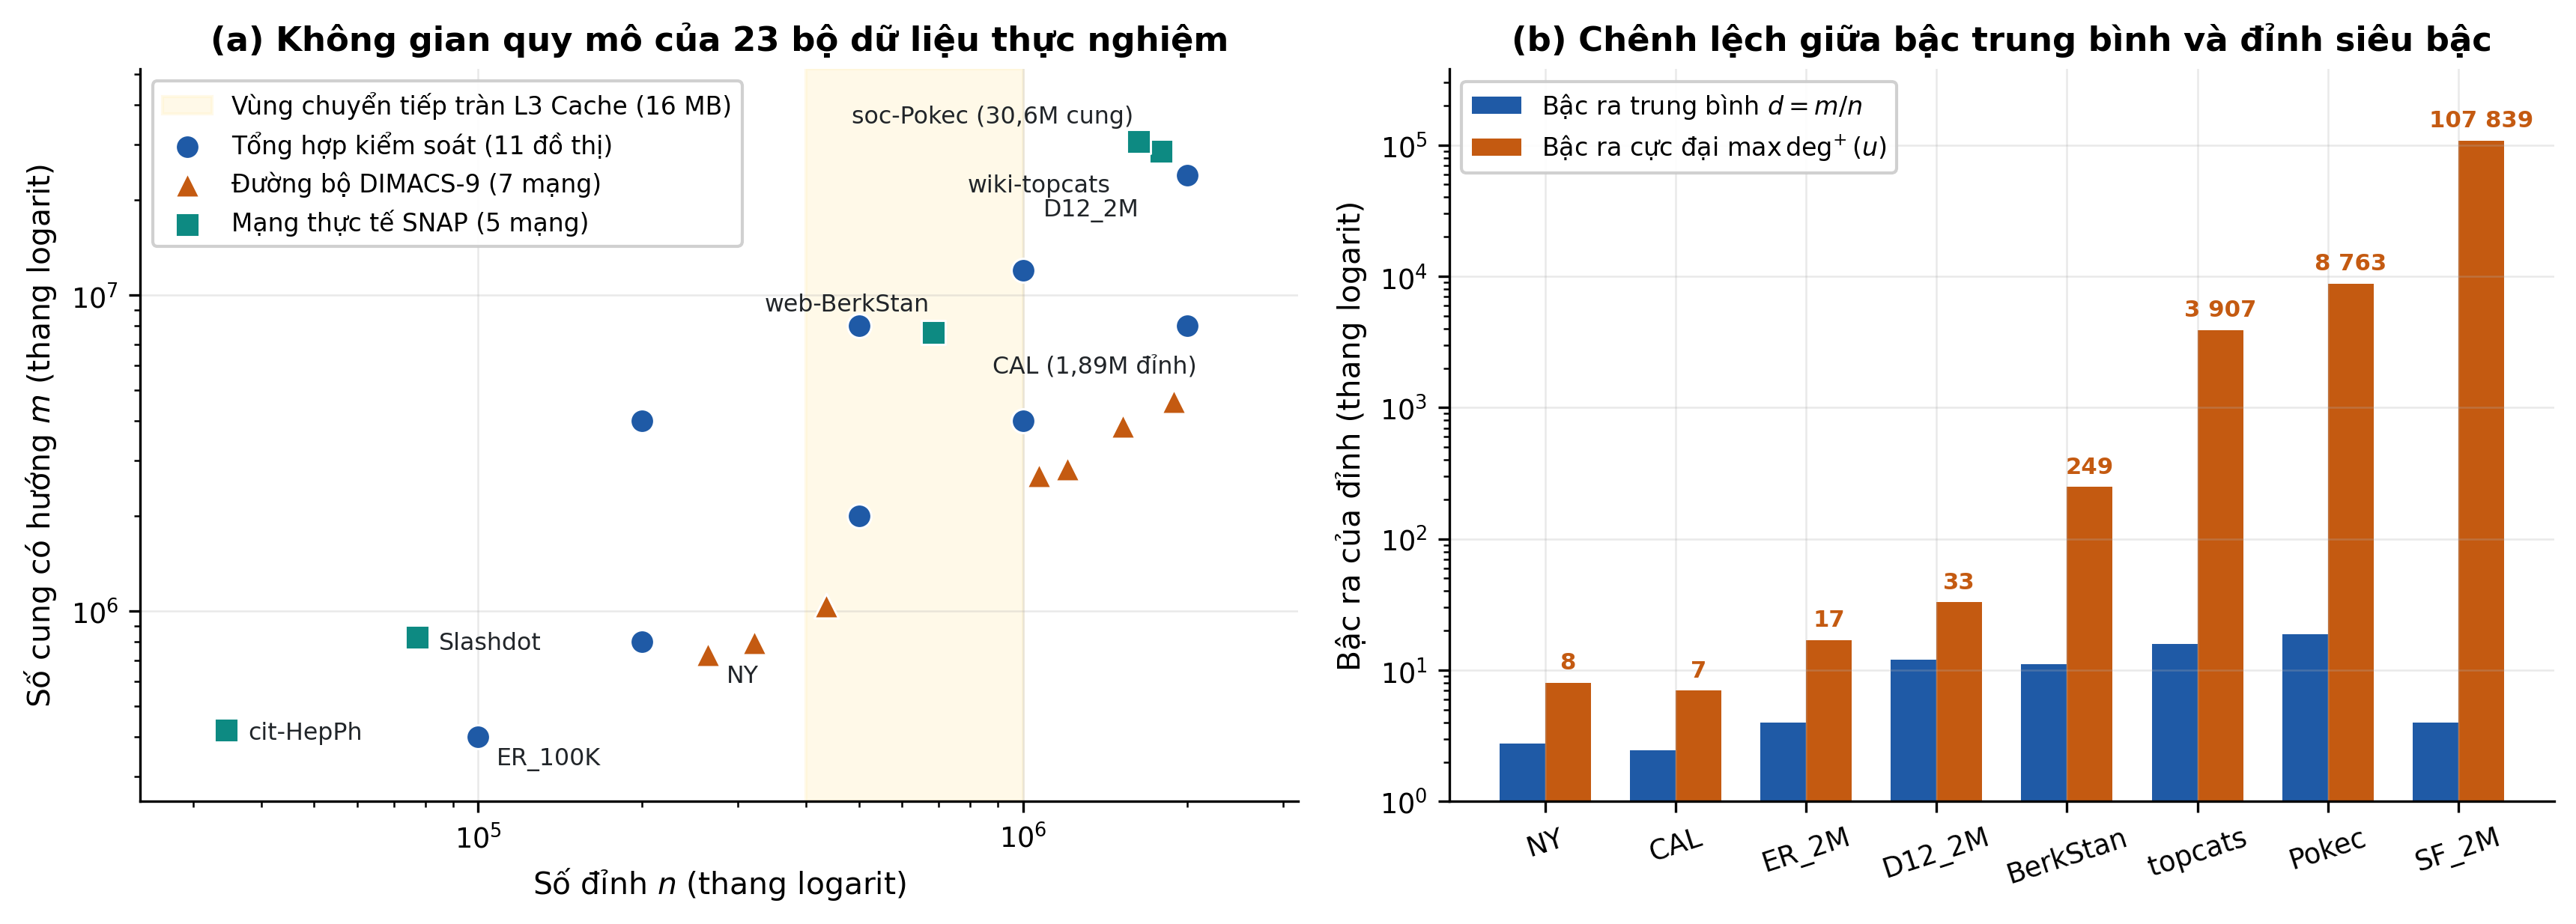
\includegraphics[width=0.96\linewidth]{image/ch3_dataset_landscape.png}
\caption{Không gian quy mô $(n, m)$ của 23 bộ dữ liệu khảo sát và sự chênh lệch giữa bậc trung bình với bậc ra cực đại.}
\label{fig:dataset_landscape}
\end{figure}

% ============================================================
% 3.3. ĐÁNH GIÁ HIỆU NĂNG TRÊN ĐỒ THỊ TỔNG HỢP KIỂM SOÁT BIẾN SỐ
% ============================================================
\section{Đánh giá hiệu năng trên đồ thị tổng hợp kiểm soát biến số}\label{sec:c3-synthetic}

Thực nghiệm trên tập đồ thị tổng hợp cho phép tách bạch rõ tác động của quy mô bộ nhớ làm việc, sự chênh lệch bậc đỉnh và mật độ cạnh lên hiệu năng đa luồng. Cụ thể, Mục~\ref{subsec:c3-syn-time} đối sánh trực tiếp thời gian giải của hệ thống với thuật toán Dijkstra tuần tự qua các mốc quy mô, sau đó Mục~\ref{subsec:c3-syn-scale} phân tích đường cong mở rộng nội tại theo số luồng và khả năng chịu tải trước các đỉnh siêu bậc.

\subsection{Thời gian giải đối sánh với Dijkstra tuần tự}\label{subsec:c3-syn-time}

Bảng~\ref{tab:syn_results} trình bày thời gian giải trung vị tính bằng mili giây của Dijkstra tuần tự và hệ thống BMSSP song song tại năm cấu hình luồng trên toàn bộ $11$ đồ thị tổng hợp. Tại quy mô nhỏ nhất \texttt{ER\_100K} với $100\,000$ đỉnh và $400\,713$ cung, toàn bộ mảng khoảng cách cùng hàng đợi nhị phân của Dijkstra nằm gọn bên trong bộ nhớ đệm L3 $16\,\mathrm{MB}$ nên Dijkstra hoàn tất trong $48{,}45\,\mathrm{ms}$, nhanh hơn nhẹ so với cấu hình tốt nhất của BMSSP ở $4$ luồng là $53{,}95\,\mathrm{ms}$ ứng với $S_{\mathrm{abs}} = 0{,}90\times$. Ở quy mô này, khối lượng cạnh trong mỗi lát đệ quy còn khiêm tốn nên phần thời gian tiết kiệm nhờ đa luồng chưa bù đắp hết chi phí duy trì cấu trúc biên phân tầng và rào chắn đồng bộ OpenMP.

\begin{table}[!htb]
\centering
\resizebox{\textwidth}{!}{%
\begin{tabular}{@{}l l r r r r r r r r@{}}
\toprule
& & & \multicolumn{5}{c}{\textbf{BMSSP theo số luồng (ms)}} & & \\
\cmidrule(lr){4-8}
\textbf{Mã đồ thị} & \textbf{Quy mô ($n$; $d$)} & \textbf{Dijkstra} & \textbf{1} & \textbf{2} & \textbf{4} & \textbf{8} & \textbf{12} & $\boldsymbol{S_{\mathrm{abs}}}$ & $\boldsymbol{S_{\mathrm{self}}}$ \\
\midrule
\texttt{ER\_100K}  & $100\mathrm{K};\; 4$  & \textbf{48,45} & 72,57 & 65,72 & 53,95 & 55,56 & 58,51 & $0{,}90\times$ & $1{,}35\times$ \\
\texttt{ER\_200K}  & $200\mathrm{K};\; 4$  & 117,19 & 174,82 & 136,68 & 113,00 & \textbf{106,75} & 110,27 & $1{,}10\times$ & $1{,}64\times$ \\
\texttt{D20\_200K} & $200\mathrm{K};\; 20$ & 254,12 & 300,91 & 244,00 & 184,86 & \textbf{163,48} & 177,86 & $1{,}55\times$ & $1{,}84\times$ \\
\texttt{ER\_500K}  & $500\mathrm{K};\; 4$  & 366,30 & 464,15 & 363,04 & 291,13 & \textbf{263,99} & 271,69 & $1{,}39\times$ & $1{,}76\times$ \\
\texttt{D16\_500K} & $500\mathrm{K};\; 16$ & 675,38 & 813,15 & 639,32 & 494,25 & \textbf{398,62} & 414,82 & $1{,}69\times$ & $2{,}04\times$ \\
\texttt{ER\_1M}    & $1{,}0\mathrm{M};\; 4$  & 746,77 & 896,54 & 705,18 & 554,14 & 500,85 & \textbf{498,66} & $1{,}50\times$ & $1{,}80\times$ \\
\texttt{SF\_1M}    & $1{,}0\mathrm{M};\; 4$  & 732,21 & 877,15 & 693,09 & 575,17 & \textbf{517,58} & 522,90 & $1{,}41\times$ & $1{,}69\times$ \\
\texttt{D12\_1M}   & $1{,}0\mathrm{M};\; 12$ & 1\,211,13 & 1\,406,66 & 1\,043,20 & 796,17 & 665,62 & \textbf{664,68} & $1{,}82\times$ & $2{,}12\times$ \\
\texttt{ER\_2M}    & $2{,}0\mathrm{M};\; 4$  & 1\,642,68 & 1\,869,91 & 1\,466,40 & 1\,119,80 & \textbf{996,52} & 1\,011,66 & $1{,}65\times$ & $1{,}88\times$ \\
\texttt{SF\_2M}    & $2{,}0\mathrm{M};\; 4$  & 1\,685,27 & 1\,913,89 & 1\,460,71 & 1\,185,89 & \textbf{1\,043,25} & 1\,057,74 & $1{,}62\times$ & $1{,}83\times$ \\
\texttt{D12\_2M}   & $2{,}0\mathrm{M};\; 12$ & 2\,645,71 & 2\,736,98 & 2\,033,11 & 1\,584,91 & 1\,330,31 & \textbf{1\,202,72} & $2{,}20\times$ & $2{,}28\times$ \\
\bottomrule
\end{tabular}%
}
\caption{Thời gian giải trung vị tính bằng ms và các hệ số tăng tốc trên 11 đồ thị tổng hợp với sai số đối chứng bằng 0.}
\label{tab:syn_results}
\end{table}

Sự đảo chiều xuất hiện ngay từ mốc $200\,000$ đỉnh và nới rộng liên tục khi quy mô đồ thị tăng lên. Trên \texttt{ER\_200K}, cấu hình $8$ luồng rút ngắn thời gian xuống $106{,}75\,\mathrm{ms}$ so với $117{,}19\,\mathrm{ms}$ của Dijkstra, đạt $S_{\mathrm{abs}} = 1{,}10\times$; khi mật độ cạnh tăng lên $d = 20$ tại \texttt{D20\_200K}, lợi thế tốc độ vọt lên $1{,}55\times$. Đáng chú ý, từ mốc $500\,000$ đỉnh trở đi, ngay cả cấu hình chỉ sử dụng $2$ luồng của BMSSP đã bắt đầu vượt qua hoặc ngang ngửa Dijkstra tuần tự, chẳng hạn $639{,}32\,\mathrm{ms}$ so với $675{,}38\,\mathrm{ms}$ trên \texttt{D16\_500K} và $2\,033{,}11\,\mathrm{ms}$ so với $2\,645{,}71\,\mathrm{ms}$ trên \texttt{D12\_2M}. Ở quy mô một triệu và hai triệu đỉnh, vùng dữ liệu hoạt động vượt xa dung lượng bộ nhớ đệm L3 khiến các thao tác hoán đổi trên cây nhị phân của Dijkstra chịu độ trễ truy cập bộ nhớ chính rất lớn. Nhờ đó, hệ thống BMSSP song song vượt Dijkstra từ $1{,}41\times$ đến $1{,}82\times$ ở nhóm một triệu đỉnh, và đạt mức tăng tốc cao nhất $S_{\mathrm{abs}} = 2{,}20\times$ trên \texttt{D12\_2M} với $24\,002\,527$ cung khi rút ngắn thời gian giải từ $2\,645{,}71\,\mathrm{ms}$ xuống còn $1\,202{,}72\,\mathrm{ms}$.

\subsection{Khả năng mở rộng nội tại và cân bằng tải trên đỉnh siêu bậc}\label{subsec:c3-syn-scale}

Hình~\ref{fig:syn_scaling} minh họa trực quan tương quan thời gian chạy ở quy mô lớn và đường cong tự tăng tốc nội tại $S_{\mathrm{self}}(p)$ khi tăng số luồng xử lý từ $1$ lên $12$. Quan sát các cột màu xanh nhạt trên Hình~\ref{fig:syn_scaling}a cho thấy ở chế độ đơn luồng $p = 1$, bản cài đặt BMSSP chỉ chậm hơn Dijkstra tuần tự từ $3{,}4\%$ trên \texttt{D12\_2M} đến khoảng $20\%$ trên đồ thị thưa $1\mathrm{M}$--$2\mathrm{M}$ đỉnh. Khoảng cách khởi điểm một luồng rất hẹp này là tiền đề quyết định giúp thuật toán nhanh chóng vượt qua bộ giải tuần tự ngay khi kích hoạt từ $2$ đến $4$ luồng công nhân.

\begin{figure}[!htb]
\centering
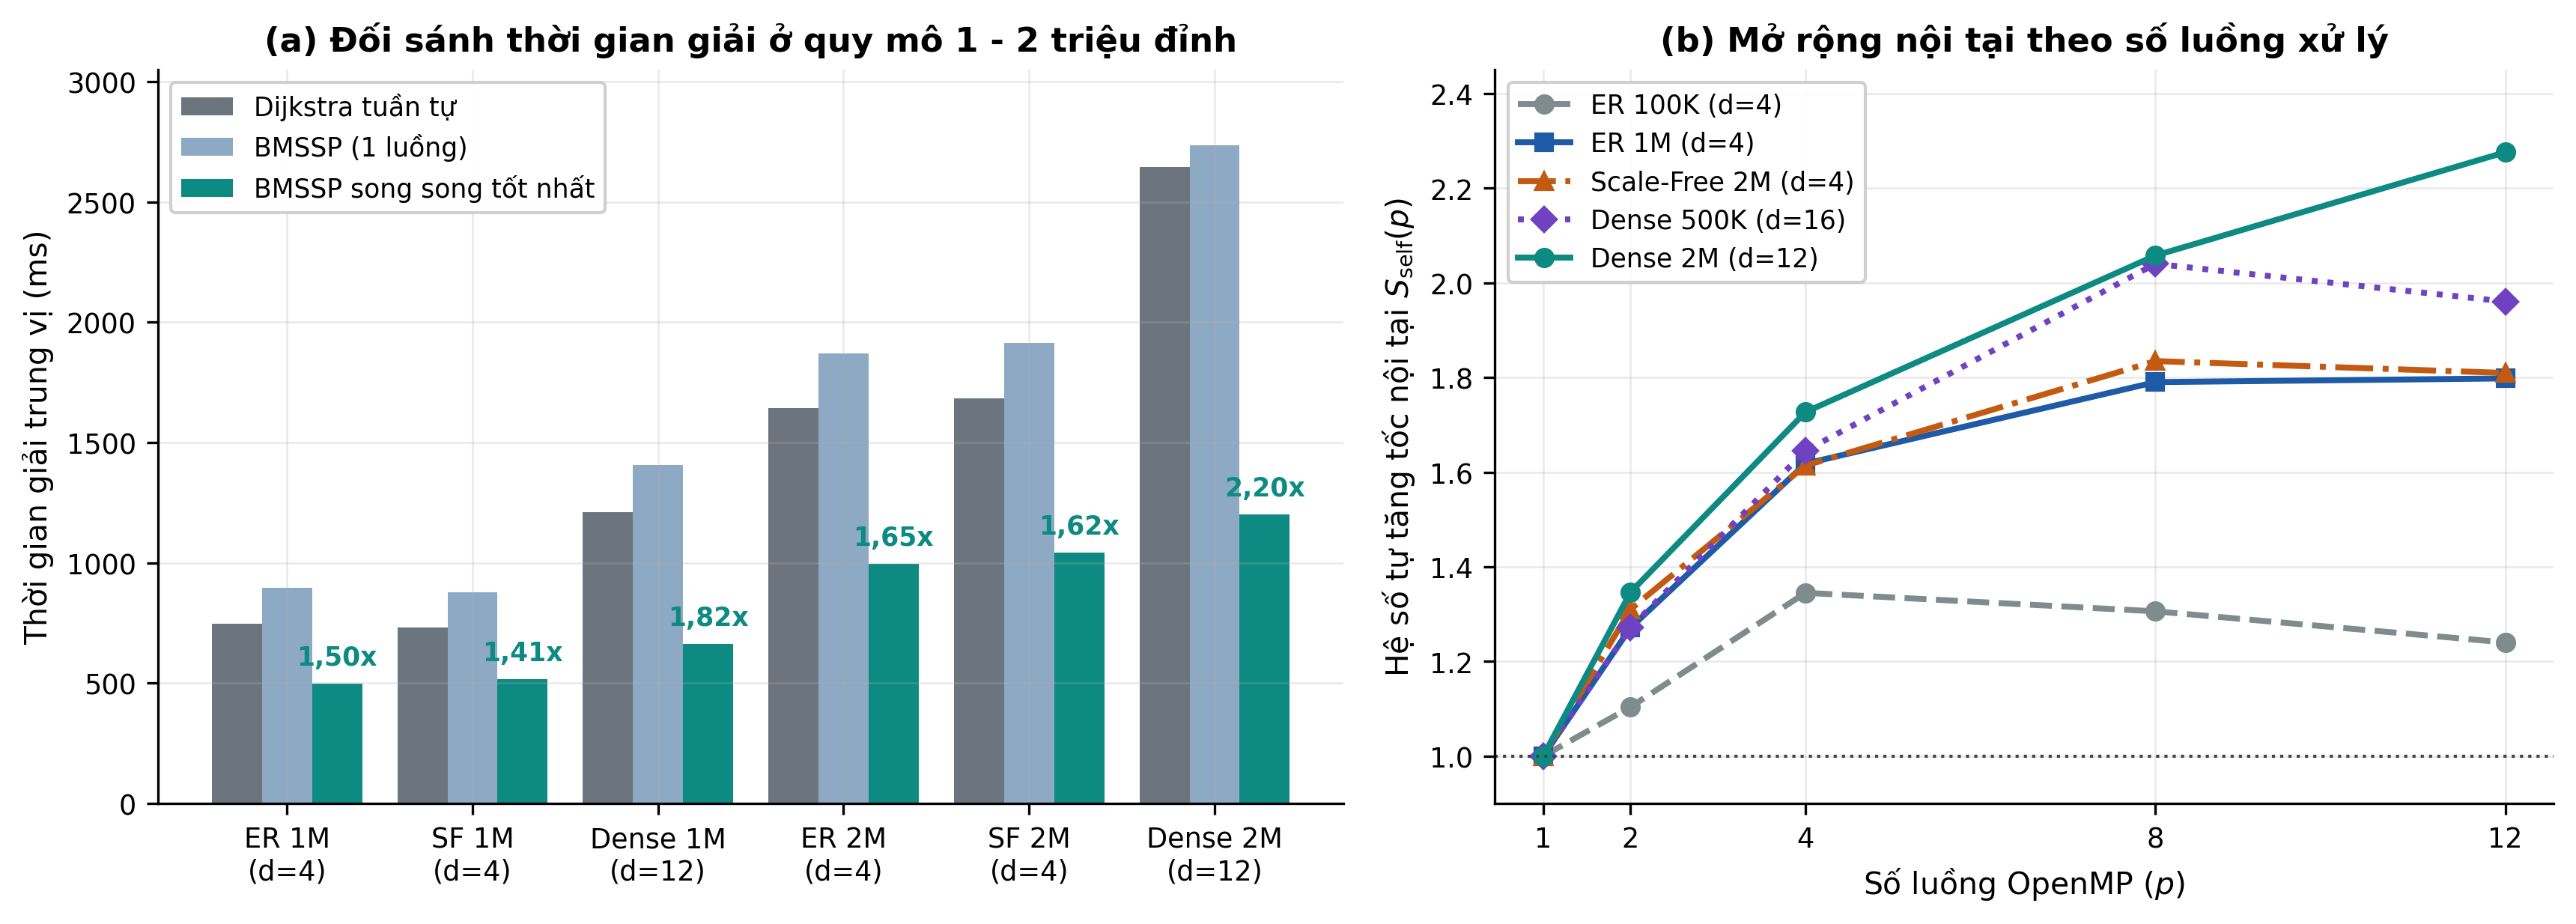
\includegraphics[width=0.96\linewidth]{image/ch3_synthetic_scaling.png}
\caption{Đối sánh thời gian giải ở quy mô 1--2 triệu đỉnh và đường cong tự tăng tốc nội tại theo số luồng trên tập đồ thị tổng hợp.}
\label{fig:syn_scaling}
\end{figure}

Về khả năng xử lý phân bố bậc lệch, phép đối sánh trên biểu đồ Hình~\ref{fig:tikz_hub_balance} giữa cặp đồ thị cùng quy mô và cùng tổng số cạnh \texttt{ER\_1M} với \texttt{SF\_1M}, cũng như \texttt{ER\_2M} với \texttt{SF\_2M}, khẳng định tính hiệu quả của chiến lược phân hoạch cạnh dựa trên mảng tổng tiền tố bậc ra và tìm kiếm nhị phân tại Mục~\ref{subsec:c2-find-pivots}. Mặc dù \texttt{SF\_2M} chứa đỉnh siêu bậc có tới $107\,839$ cung đi ra so với mức tối đa chỉ $17$ cung ở \texttt{ER\_2M}, thời gian giải tốt nhất ở $8$ luồng chỉ chênh lệch $4{,}7\%$, tương ứng $1\,043{,}25\,\mathrm{ms}$ so với $996{,}52\,\mathrm{ms}$, hoàn toàn không xảy ra hiện tượng một luồng đơn lẻ bị kẹt tại đỉnh trung tâm làm đình trệ rào chắn cuối pha.

\begin{figure}[!htb]
\centering
\resizebox{0.96\textwidth}{!}{%
\begin{tikzpicture}[>=latex, font=\scriptsize]
    % Chú giải màu phía trên
    \fill[gray!70!black] (0.2, 5.85) rectangle (0.65, 6.10);
    \node[anchor=west] at (0.75, 5.97) {Dijkstra tuần tự};
    \fill[blue!35!gray!65] (3.7, 5.85) rectangle (4.15, 6.10);
    \node[anchor=west] at (4.25, 5.97) {BMSSP 1 luồng};
    \fill[teal!75!black] (7.2, 5.85) rectangle (7.65, 6.10);
    \node[anchor=west] at (7.75, 5.97) {BMSSP 8 luồng};

    % Trục và đường lưới dọc (thang 1.0 cm = 200 ms, từ 0 đến 2000 ms -> 0 đến 10.0 cm)
    \foreach \v/\lbl in {0/0, 2.5/500, 5.0/1\,000, 7.5/1\,500, 10.0/2\,000} {
        \draw[gray!28, thin] (\v, 0.25) -- (\v, 5.55);
        \draw[black!70] (\v, 0.25) -- (\v, 0.15);
        \node[anchor=north] at (\v, 0.12) {\lbl};
    }
    \draw[->, thick, black!80] (0, 0.25) -- (10.85, 0.25);
    \draw[thick, black!80] (0, 0.25) -- (0, 5.55);
    \node[anchor=north, font=\scriptsize\bfseries] at (5.2, -0.32) {Thời gian giải trung vị (ms)};

    % Nhóm 1: ER_1M (y trung tâm = 4.90)
    \node[anchor=east, align=right, text width=3.3cm] at (-0.18, 4.90) {\textbf{\texttt{ER\_1M}} ($1\mathrm{M}$ đỉnh)\\Bậc tối đa: $17$};
    \fill[gray!70!black]   (0, 5.10) rectangle (3.734, 5.34); \node[anchor=west] at (3.82, 5.22) {746,8};
    \fill[blue!35!gray!65] (0, 4.78) rectangle (4.483, 5.02); \node[anchor=west] at (4.57, 4.90) {896,5};
    \fill[teal!75!black]   (0, 4.46) rectangle (2.504, 4.70); \node[anchor=west, text=teal!65!black, font=\scriptsize\bfseries] at (2.59, 4.58) {500,9 ms ($1{,}49\times$)};

    % Nhóm 2: SF_1M (y trung tâm = 3.60)
    \node[anchor=east, align=right, text width=3.3cm] at (-0.18, 3.60) {\textbf{\texttt{SF\_1M}} ($1\mathrm{M}$ đỉnh)\\Bậc tối đa: $62\,550$};
    \fill[gray!70!black]   (0, 3.80) rectangle (3.661, 4.04); \node[anchor=west] at (3.75, 3.92) {732,2};
    \fill[blue!35!gray!65] (0, 3.48) rectangle (4.386, 3.72); \node[anchor=west] at (4.47, 3.60) {877,2};
    \fill[teal!75!black]   (0, 3.16) rectangle (2.588, 3.40); \node[anchor=west, text=teal!65!black, font=\scriptsize\bfseries] at (2.68, 3.28) {517,6 ms ($1{,}41\times$)};

    % Nhóm 3: ER_2M (y trung tâm = 2.30)
    \node[anchor=east, align=right, text width=3.3cm] at (-0.18, 2.30) {\textbf{\texttt{ER\_2M}} ($2\mathrm{M}$ đỉnh)\\Bậc tối đa: $17$};
    \fill[gray!70!black]   (0, 2.50) rectangle (8.213, 2.74); \node[anchor=west] at (8.30, 2.62) {1\,642,7};
    \fill[blue!35!gray!65] (0, 2.18) rectangle (9.350, 2.42); \node[anchor=west] at (9.44, 2.30) {1\,869,9};
    \fill[teal!75!black]   (0, 1.86) rectangle (4.983, 2.10); \node[anchor=west, text=teal!65!black, font=\scriptsize\bfseries] at (5.07, 1.98) {996,5 ms ($1{,}65\times$)};

    % Nhóm 4: SF_2M (y trung tâm = 1.00)
    \node[anchor=east, align=right, text width=3.3cm] at (-0.18, 1.00) {\textbf{\texttt{SF\_2M}} ($2\mathrm{M}$ đỉnh)\\Bậc tối đa: $107\,839$};
    \fill[gray!70!black]   (0, 1.20) rectangle (8.426, 1.44); \node[anchor=west] at (8.51, 1.32) {1\,685,3};
    \fill[blue!35!gray!65] (0, 0.88) rectangle (9.569, 1.12); \node[anchor=west] at (9.65, 1.00) {1\,913,9};
    \fill[teal!75!black]   (0, 0.56) rectangle (5.216, 0.80); \node[anchor=west, text=teal!65!black, font=\scriptsize\bfseries] at (5.30, 0.68) {1\,043,2 ms ($1{,}62\times$)};
\end{tikzpicture}%
}
\caption{Đối sánh cân bằng tải giữa đồ thị đồng nhất Erd\H{o}s--R\'{e}nyi và đồ thị lệch bậc chứa đỉnh siêu bậc lên tới 107\,839 cung.}
\label{fig:tikz_hub_balance}
\end{figure}

Trên Hình~\ref{fig:syn_scaling}b, diễn biến giữa mức $8$ luồng và $12$ luồng phản ánh trung thực đặc trưng phần cứng của vi xử lý $6$ lõi vật lý sử dụng công nghệ đa luồng đồng thời SMT. Với các đồ thị thưa $d = 4$, mỗi cạnh chỉ thực hiện vài phép tính số học đơn giản đi kèm truy cập bộ nhớ rải rác nên băng thông bộ nhớ của $6$ lõi vật lý sớm bão hòa tại $8$ luồng với $S_{\mathrm{self}} \approx 1{,}80\times$--$1{,}88\times$. Ngược lại, trên đồ thị mật độ cao \texttt{D12\_2M} gồm $24$ triệu cung, các dải kề CSR dài giúp bộ nạp trước phần cứng hoạt động hiệu quả và nâng tỷ lệ tính toán trên mỗi dòng bộ nhớ đệm, cho phép $12$ luồng SMT tận dụng các chu kỳ trễ đường ống để đẩy hệ số tự tăng tốc nội tại lên mức cao nhất $S_{\mathrm{self}}(12) = 2{,}28\times$.

% ============================================================
% 3.4. ĐÁNH GIÁ HIỆU NĂNG TRÊN CÁC MẠNG THỰC TẾ
% ============================================================
\section{Đánh giá hiệu năng trên các mạng thực tế}\label{sec:c3-realworld}

Sau khi xác lập hành vi của hệ thống trên dữ liệu tổng hợp, bước kiểm định quan trọng tiếp theo là đặt thuật toán vào hai lớp mạng thực tế có cấu trúc đối lập nhau. Theo hướng đó, Mục~\ref{subsec:c3-road} khảo sát giới hạn thực thi của mô hình cắt lát khoảng cách trên $7$ mạng đường bộ phẳng bậc rất thấp, tiếp theo Mục~\ref{subsec:c3-snap} làm rõ quá trình chuyển pha và bứt phá tốc độ trên $5$ mạng liên kết thực tế bậc cao của Stanford SNAP.

\subsection{Giới hạn trên mạng đường bộ phẳng bậc thấp DIMACS-9}\label{subsec:c3-road}

Bảng~\ref{tab:road_results} và Hình~\ref{fig:dimacs_road} tổng hợp kết quả đo trên $7$ mạng giao thông đường bộ khu vực từ \texttt{NY} đến \texttt{CAL}. Khác biệt rõ rệt với tập đồ thị ngẫu nhiên ở mục trước, trên cả bảy mạng đường bộ có bậc ra trung bình nằm trong khoảng $2{,}34$ đến $2{,}76$, thuật toán Dijkstra tuần tự luôn duy trì thời gian giải thấp hơn. Ở cấu hình đa luồng tốt nhất từ $8$ đến $12$ luồng, thời gian của BMSSP gấp từ $1{,}70$ đến $2{,}67$ lần thời gian của Dijkstra, trong khi hệ số tự tăng tốc nội tại $S_{\mathrm{self}}$ chỉ đạt mức khiêm tốn từ $1{,}07\times$ đến $1{,}23\times$.

\begin{table}[!htb]
\centering
\resizebox{\textwidth}{!}{%
\begin{tabular}{@{}l l r r r r r r r r r@{}}
\toprule
& & & & & \multicolumn{4}{c}{\textbf{BMSSP theo số luồng (ms)}} & & \\
\cmidrule(lr){6-9}
\textbf{Mã} & \textbf{Khu vực} & \textbf{Số đỉnh $n$} & \textbf{Số cung $m$} & \textbf{Dijkstra} & \textbf{1} & \textbf{4} & \textbf{8} & \textbf{12} & $\boldsymbol{T_{\mathrm{par}}/T_{\mathrm{base}}}$ & $\boldsymbol{S_{\mathrm{self}}}$ \\
\midrule
\texttt{NY}  & New York       & 264\,346    & 730\,100    & \textbf{63,71}  & 201,77 & 178,68 & 174,09 & 166,87 & $2{,}62\times$ & $1{,}21\times$ \\
\texttt{BAY} & Vịnh SF        & 321\,270    & 794\,830    & \textbf{73,20}  & 223,30 & 203,55 & 195,39 & 196,59 & $2{,}67\times$ & $1{,}14\times$ \\
\texttt{COL} & Colorado       & 435\,666    & 1\,042\,400 & \textbf{101,79} & 269,06 & 238,61 & 241,02 & 236,77 & $2{,}33\times$ & $1{,}14\times$ \\
\texttt{FLA} & Florida        & 1\,070\,376 & 2\,687\,902 & \textbf{226,74} & 638,99 & 577,49 & 541,95 & 563,35 & $2{,}39\times$ & $1{,}18\times$ \\
\texttt{NW}  & Tây Bắc Mỹ     & 1\,207\,945 & 2\,820\,776 & \textbf{295,80} & 659,74 & 616,08 & 614,24 & 615,09 & $2{,}08\times$ & $1{,}07\times$ \\
\texttt{NE}  & Đông Bắc Mỹ    & 1\,524\,453 & 3\,857\,376 & \textbf{445,99} & 936,50 & 803,36 & 758,88 & 760,91 & $1{,}70\times$ & $1{,}23\times$ \\
\texttt{CAL} & California--NV & 1\,890\,815 & 4\,620\,230 & \textbf{482,93} & 1\,077,89 & 985,64 & 914,01 & 891,43 & $1{,}85\times$ & $1{,}21\times$ \\
\bottomrule
\end{tabular}%
}
\caption{Thời gian giải trung vị tính bằng ms và tỷ số tốc độ trên 7 mạng đường bộ Hoa Kỳ thuộc bộ chuẩn DIMACS-9.}
\label{tab:road_results}
\end{table}

Hiện tượng này bắt nguồn trực tiếp từ sự tương tác giữa cấu trúc hình học phẳng hai chiều với hai giới hạn phần cứng đã phân tích tại Bảng~\ref{tab:theory_vs_hardware} của Chương~\ref{chap:parallel_bmssp}. Thứ nhất, mặt sóng lan truyền khoảng cách trên mạng giao lộ phẳng chỉ là một vành đai địa lý mỏng gồm vài chục đến vài trăm đỉnh ở mỗi thời điểm; cộng thêm bậc ra trung bình chỉ khoảng $2{,}5$, tổng số cung hoạt động $N_{\mathrm{act}}$ trong phần lớn các bước lặp của \textsc{FindPivots} và các lời gọi đệ quy tầng sâu đều rơi xuống dưới ngưỡng độ hạt $\Theta_{\mathrm{cutoff}} = 2048$. Hệ quả là phần lớn quá trình giải tự động chuyển về thực thi tuần tự trong khi vẫn phải gánh chi phí phân tách đệ quy nhiều tầng và quản lý cấu trúc biên $\mathcal{D}$. Thứ hai, các giao lộ gần nhau ngoài thực địa trong dữ liệu đường bộ thường có mã chỉ số đỉnh nằm sát nhau trên mảng bộ nhớ, đồng thời kích thước hàng đợi ưu tiên của Dijkstra trên đồ thị phẳng luôn rất nhỏ so với tổng số đỉnh. Nhờ tính cục bộ không gian cao đó, Dijkstra giải xong mạng \texttt{FLA} $1{,}07\mathrm{M}$ đỉnh chỉ trong $226{,}74\,\mathrm{ms}$, nhanh hơn gấp ba lần so với chính Dijkstra trên đồ thị ngẫu nhiên \texttt{ER\_1M} có cùng số đỉnh là $746{,}77\,\mathrm{ms}$.

\begin{figure}[!htb]
\centering
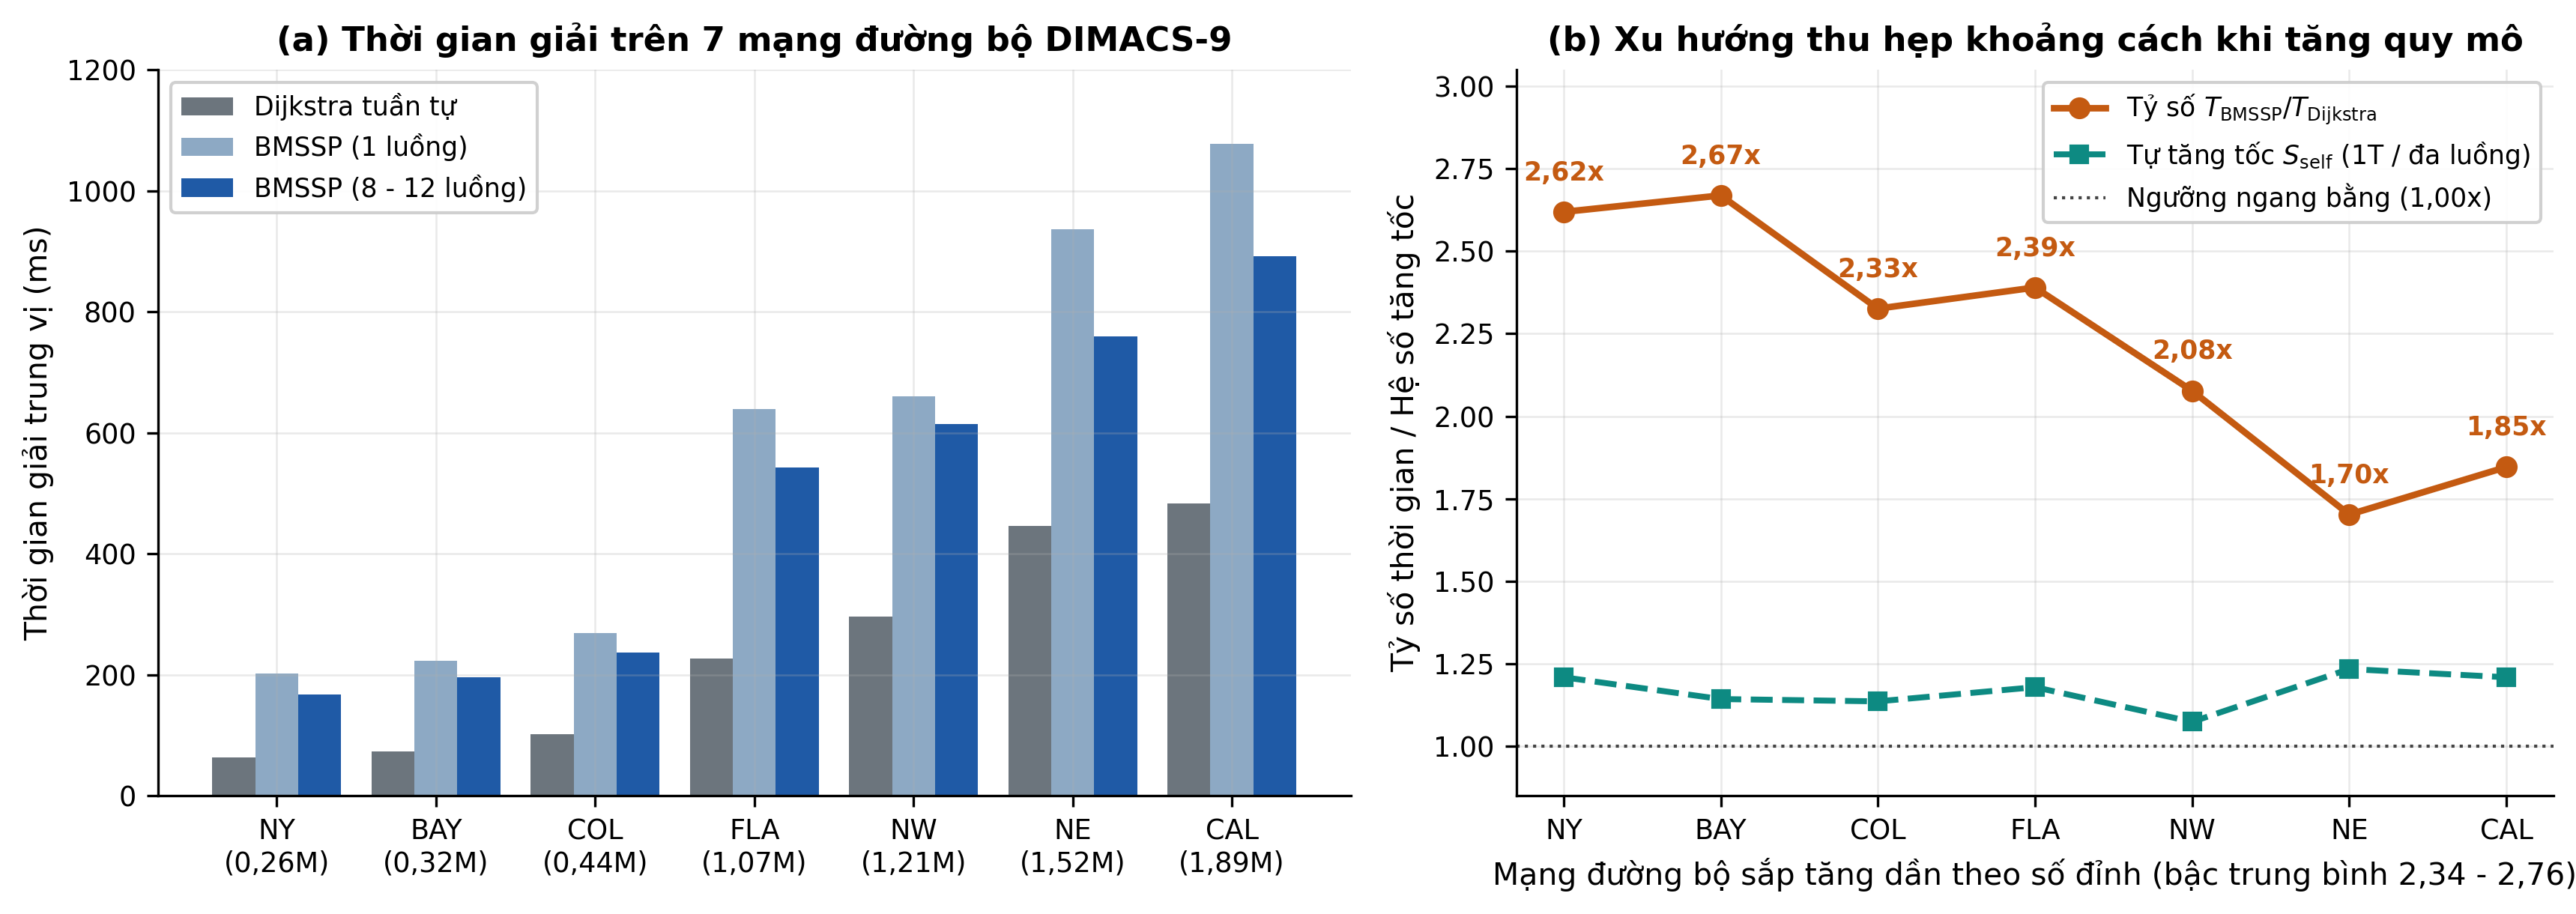
\includegraphics[width=0.96\linewidth]{image/ch3_dimacs_road.png}
\caption{Thời gian giải và xu hướng giảm dần tỷ số $T_{\mathrm{BMSSP}} / T_{\mathrm{Dijkstra}}$ khi quy mô đỉnh tăng trên 7 mạng đường bộ DIMACS-9.}
\label{fig:dimacs_road}
\end{figure}

Mặc dù chưa vượt qua Dijkstra ở dải bậc cực thấp này, đường màu cam trên Hình~\ref{fig:dimacs_road}b vẫn bộc lộ một xu hướng hội tụ nhất quán theo quy mô đỉnh. Khi kích thước mạng tăng gấp sáu lần từ \texttt{BAY} với $0{,}32\mathrm{M}$ đỉnh lên hành lang đô thị Đông Bắc \texttt{NE} với $1{,}52\mathrm{M}$ đỉnh và \texttt{CAL} với $1{,}89\mathrm{M}$ đỉnh, vành đai mặt sóng mở rộng hơn giúp hệ số tự tăng tốc nội tại nhích lên $1{,}21\times$--$1{,}23\times$, đồng thời mảng trạng thái vượt quá bộ nhớ đệm L3 làm giảm lợi thế cục bộ của Dijkstra. Qua đó, tỷ số thời gian $T_{\mathrm{BMSSP}} / T_{\mathrm{Dijkstra}}$ thu hẹp đều đặn từ mức $2{,}67\times$ ở \texttt{BAY} xuống $2{,}33\times$ ở \texttt{COL}, $2{,}08\times$ ở \texttt{NW} và chỉ còn $1{,}70\times$--$1{,}85\times$ tại \texttt{NE} và \texttt{CAL}.

\subsection{Điểm đảo chiều và ưu thế trên mạng thực tế bậc cao Stanford SNAP}\label{subsec:c3-snap}

Khi chuyển từ mạng giao thông phẳng sang các mạng thông tin và xã hội thực tế có bậc trung bình từ $10{,}71$ đến $18{,}75$ trong Bảng~\ref{tab:snap_results}, bức tranh hiệu năng thay đổi căn bản và tái hiện rõ nét một đường cong chuyển pha đơn điệu theo quy mô đỉnh như thể hiện trên Hình~\ref{fig:snap_highdeg} và Hình~\ref{fig:tikz_snap_bars}.

\begin{table}[!htb]
\centering
\resizebox{\textwidth}{!}{%
\begin{tabular}{@{}l r r r r r r r r r r@{}}
\toprule
& & & & \multicolumn{5}{c}{\textbf{BMSSP theo số luồng (ms)}} & & \\
\cmidrule(lr){5-9}
\textbf{Bộ dữ liệu} & \textbf{Số đỉnh $n$} & \textbf{Bậc $d$} & \textbf{Dijkstra} & \textbf{1} & \textbf{2} & \textbf{4} & \textbf{8} & \textbf{12} & $\boldsymbol{S_{\mathrm{abs}}}$ & $\boldsymbol{S_{\mathrm{self}}}$ \\
\midrule
\texttt{cit-HepPh}        & 34\,546     & 12,20 & \textbf{6,41}  & 19,10 & 19,75 & 18,20 & 21,20 & 19,50 & $0{,}35\times$ & $1{,}05\times$ \\
\texttt{soc-Slashdot0811} & 77\,360     & 10,71 & \textbf{53,06} & 72,95 & 80,62 & 73,23 & 66,20 & 64,86 & $0{,}82\times$ & $1{,}12\times$ \\
\texttt{web-BerkStan}     & 685\,230    & 11,09 & 299,01 & 464,93 & 447,04 & 403,07 & \textbf{291,25} & 299,11 & $1{,}03\times$ & $1{,}60\times$ \\
\texttt{wiki-topcats}     & 1\,791\,489 & 15,91 & 2\,219,93 & 2\,535,15 & 1\,906,69 & 1\,421,54 & 1\,336,99 & \textbf{1\,315,10} & $1{,}69\times$ & $1{,}93\times$ \\
\texttt{soc-Pokec}        & 1\,632\,803 & 18,75 & 2\,474,98 & 2\,520,72 & 1\,859,25 & 1\,442,74 & 1\,462,64 & \textbf{1\,351,73} & $1{,}83\times$ & $1{,}86\times$ \\
\bottomrule
\end{tabular}%
}
\caption{Thời gian giải trung vị tính bằng ms và hệ số tăng tốc trên 5 mạng thực tế bậc cao từ kho dữ liệu Stanford SNAP.}
\label{tab:snap_results}
\end{table}

Ở hai mạng quy mô nhỏ dưới $100\,000$ đỉnh, dữ liệu nằm trọn trong bộ nhớ đệm tốc độ cao của vi xử lý. Trên mạng trích dẫn có hướng không chu trình \texttt{cit-HepPh}, nguồn chỉ đi tới $20\,507$ đỉnh nên Dijkstra kết thúc sau $6{,}41\,\mathrm{ms}$, trong khi BMSSP mất $18{,}20\,\mathrm{ms}$ ứng với $S_{\mathrm{abs}} = 0{,}35\times$ do chi phí cố định khởi tạo vùng làm việc cho các tầng đệ quy. Tuy nhiên, ngay khi quy mô tăng lên $77\,360$ đỉnh liên thông toàn phần trên mạng cộng đồng \texttt{soc-Slashdot0811}, thời gian của Dijkstra tăng vọt hơn tám lần lên $53{,}06\,\mathrm{ms}$, còn BMSSP chỉ tăng lên $64{,}86\,\mathrm{ms}$, kéo hệ số $S_{\mathrm{abs}}$ tiến sát ngưỡng cân bằng ở mức $0{,}82\times$.

\begin{figure}[!htb]
\centering
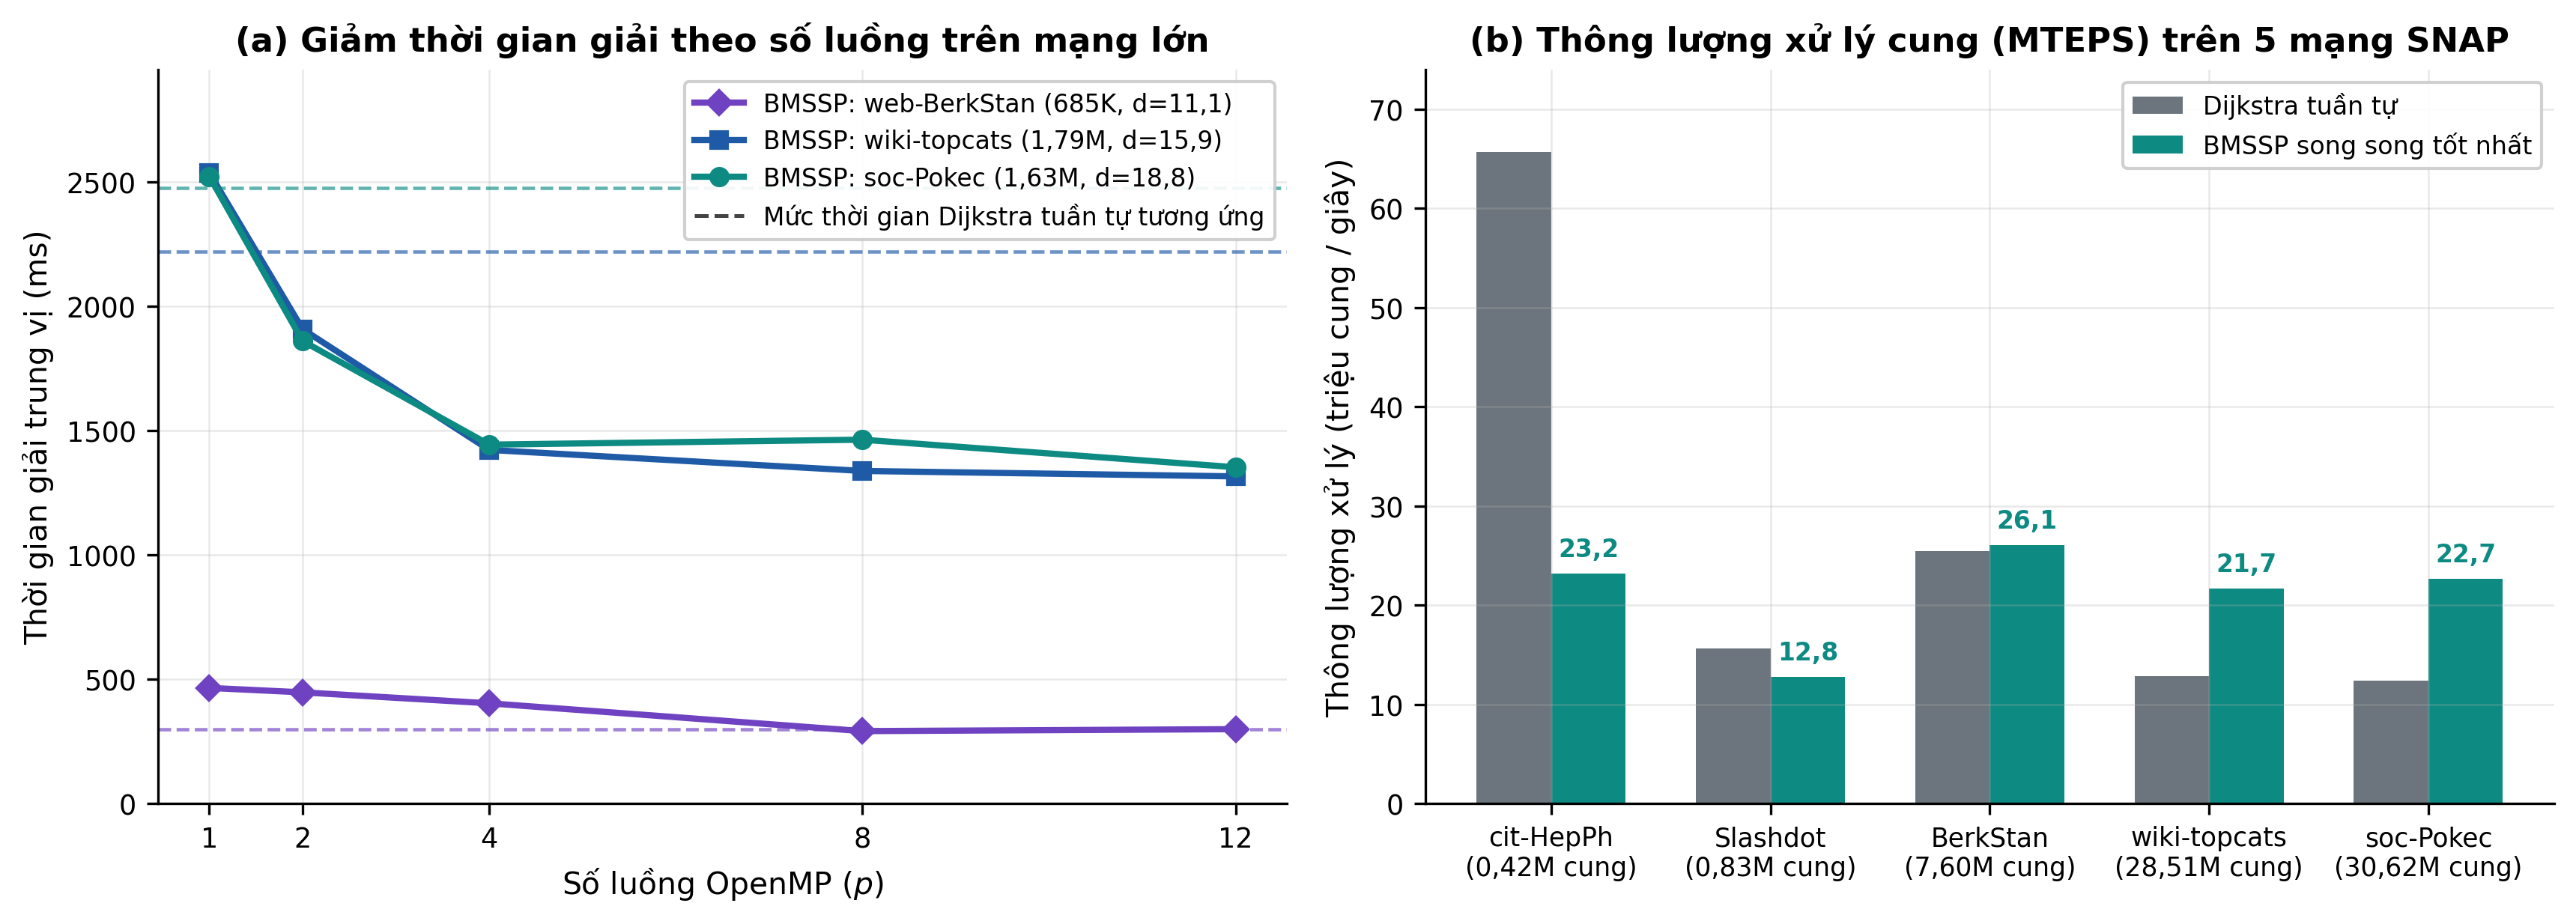
\includegraphics[width=0.96\linewidth]{image/ch3_snap_highdeg.png}
\caption{Đường cong giảm thời gian giải theo số luồng và thông lượng xử lý triệu cung mỗi giây trên 5 mạng thực tế Stanford SNAP.}
\label{fig:snap_highdeg}
\end{figure}

Điểm cắt thực nghiệm trên dữ liệu thực tế xuất hiện tại mạng liên kết Web \texttt{web-BerkStan} gồm $685\,230$ đỉnh và $7\,600\,595$ cung, trong đó có $459\,831$ đỉnh tới được từ nguồn. Dù các trang Web thuộc cùng hệ thống tên miền có tính phân cụm cục bộ rất cao tạo thuận lợi cho bộ nhớ đệm của Dijkstra, khối lượng cạnh trên mỗi lát của \texttt{web-BerkStan} đã đủ lớn để kích hoạt hiệu quả vùng công nhân OpenMP với $S_{\mathrm{self}}(8) = 1{,}60\times$, giúp BMSSP ở $8$ luồng đạt $291{,}25\,\mathrm{ms}$ và chính thức vượt nhẹ Dijkstra tuần tự ở mức $299{,}01\,\mathrm{ms}$ tương ứng $S_{\mathrm{abs}} = 1{,}03\times$.

\begin{figure}[!htb]
\centering
\resizebox{0.94\textwidth}{!}{%
\begin{tikzpicture}[>=latex, font=\scriptsize]
    % Chú giải phía trên
    \fill[teal!75!black] (0.8, 5.05) rectangle (1.25, 5.30);
    \node[anchor=west] at (1.35, 5.17) {Tăng tốc so với Dijkstra $S_{\mathrm{abs}}$};
    \fill[blue!38!gray!65] (5.5, 5.05) rectangle (5.95, 5.30);
    \node[anchor=west] at (6.05, 5.17) {Tự tăng tốc nội tại $S_{\mathrm{self}}$};
    \draw[red!70!black, dashed, very thick] (9.6, 5.17) -- (10.25, 5.17);
    \node[anchor=west, text=red!70!black] at (10.35, 5.17) {Ngưỡng cân bằng $1{,}00\times$};

    % Lưới ngang (thang 1,00x = 2,20 cm -> 2,00x = 4,40 cm)
    \foreach \yv/\ylbl in {0.0/0{,}00, 1.10/0{,}50, 2.20/1{,}00, 3.30/1{,}50, 4.40/2{,}00} {
        \draw[gray!26, thin] (0.4, \yv) -- (12.6, \yv);
        \draw[black!70] (0.4, \yv) -- (0.30, \yv);
        \node[anchor=east] at (0.26, \yv) {$\ylbl\times$};
    }
    \draw[->, thick, black!80] (0.4, 0) -- (12.85, 0);
    \draw[->, thick, black!80] (0.4, 0) -- (0.4, 4.85);
    \node[rotate=90, anchor=south, font=\scriptsize\bfseries] at (-0.65, 2.40) {Hệ số tăng tốc};

    % Đường ngưỡng 1,00x
    \draw[red!70!black, dashed, very thick] (0.4, 2.20) -- (12.6, 2.20);

    % Cụm 1: cit-HepPh (xc = 1.65)
    \fill[gray!65!black]   (1.03, 0) rectangle (1.61, 0.77);
    \fill[blue!38!gray!65] (1.69, 0) rectangle (2.27, 2.31);
    \node[anchor=south, font=\scriptsize\bfseries, text=black!75] at (1.32, 0.79) {$0{,}35\times$};
    \node[anchor=south, text=blue!50!black] at (1.98, 2.33) {$1{,}05\times$};
    \node[anchor=north, align=center] at (1.65, -0.08) {\texttt{cit-HepPh}\\($34{,}5\mathrm{K}$)};

    % Cụm 2: Slashdot0811 (xc = 4.05)
    \fill[gray!65!black]   (3.43, 0) rectangle (4.01, 1.80);
    \fill[blue!38!gray!65] (4.09, 0) rectangle (4.67, 2.46);
    \node[anchor=south, font=\scriptsize\bfseries, text=black!75] at (3.72, 1.82) {$0{,}82\times$};
    \node[anchor=south, text=blue!50!black] at (4.38, 2.48) {$1{,}12\times$};
    \node[anchor=north, align=center] at (4.05, -0.08) {\texttt{Slashdot0811}\\($77{,}4\mathrm{K}$)};

    % Cụm 3: web-BerkStan (xc = 6.45)
    \fill[orange!80!black] (5.83, 0) rectangle (6.41, 2.27);
    \fill[blue!38!gray!65] (6.49, 0) rectangle (7.07, 3.52);
    \node[anchor=south, font=\scriptsize\bfseries, text=orange!75!black] at (6.12, 2.31) {$1{,}03\times$};
    \node[anchor=south, text=blue!50!black] at (6.78, 3.54) {$1{,}60\times$};
    \node[anchor=north, align=center] at (6.45, -0.08) {\texttt{web-BerkStan}\\($685\mathrm{K}$)};

    % Cụm 4: wiki-topcats (xc = 8.85)
    \fill[teal!75!black]   (8.23, 0) rectangle (8.81, 3.72);
    \fill[blue!38!gray!65] (8.89, 0) rectangle (9.47, 4.25);
    \node[anchor=south, font=\scriptsize\bfseries, text=teal!65!black] at (8.52, 3.74) {$1{,}69\times$};
    \node[anchor=south, text=blue!50!black] at (9.18, 4.27) {$1{,}93\times$};
    \node[anchor=north, align=center] at (8.85, -0.08) {\texttt{wiki-topcats}\\($1{,}79\mathrm{M}$)};

    % Cụm 5: soc-Pokec (xc = 11.25)
    \fill[teal!75!black]   (10.63, 0) rectangle (11.21, 4.03);
    \fill[blue!38!gray!65] (11.29, 0) rectangle (11.87, 4.09);
    \node[anchor=south, font=\scriptsize\bfseries, text=teal!65!black] at (10.92, 4.05) {$1{,}83\times$};
    \node[anchor=south, text=blue!50!black] at (11.58, 4.11) {$1{,}86\times$};
    \node[anchor=north, align=center] at (11.25, -0.08) {\texttt{soc-Pokec}\\($1{,}63\mathrm{M}$)};
\end{tikzpicture}%
}
\caption{Quá trình chuyển pha đơn điệu của hệ số tăng tốc $S_{\mathrm{abs}}$ và $S_{\mathrm{self}}$ theo quy mô tăng dần trên 5 mạng thực tế SNAP.}
\label{fig:tikz_snap_bars}
\end{figure}

Khi tiến vào vùng quy mô trên $1{,}6$ triệu đỉnh và xấp xỉ $30$ triệu cung của hai mạng \texttt{wiki-topcats} và \texttt{soc-Pokec}, ưu thế của kiến trúc BMSSP song song thể hiện toàn diện trên cả thời gian thực thi lẫn thông lượng xử lý cung trên Hình~\ref{fig:snap_highdeg}b. Ngay ở cấu hình một luồng, thời gian của BMSSP trên \texttt{soc-Pokec} là $2\,520{,}72\,\mathrm{ms}$, xấp xỉ ngang bằng mức $2\,474{,}98\,\mathrm{ms}$ của Dijkstra. Khi mở rộng lên $12$ luồng, thời gian giải giảm mạnh xuống còn $1\,315{,}10\,\mathrm{ms}$ trên \texttt{wiki-topcats} ứng với thông lượng $21{,}7$ triệu cung mỗi giây và $1\,351{,}73\,\mathrm{ms}$ trên \texttt{soc-Pokec} ứng với $22{,}7$ triệu cung mỗi giây, vượt xa mức thông lượng bị suy giảm còn khoảng $12{,}4$--$12{,}8$ triệu cung mỗi giây của Dijkstra tuần tự. Kết quả là hệ thống giải nhanh hơn Dijkstra lần lượt $1{,}69\times$ và $1{,}83\times$, tiết kiệm hơn $0{,}90$ đến $1{,}12$ giây cho mỗi truy vấn đường đi ngắn nhất.

% ============================================================
% 3.5. PHÂN TÍCH TỔNG HỢP QUY LUẬT (N, D) VÀ NÚT THẮT HỆ THỐNG
% ============================================================
\section{Phân tích tổng hợp mối liên hệ giữa quy mô đỉnh, bậc đỉnh và nút thắt hệ thống}\label{sec:c3-tong-hop}

Kết hợp toàn bộ $23$ phép đo từ ba nhóm dữ liệu cho phép giải thích thống nhất vì sao cùng một kiến trúc BMSSP song song lại chậm hơn trên mạng đường bộ nhưng vượt xa Dijkstra trên mạng xã hội và đồ thị bậc cao. Để làm sáng tỏ bản chất này, Mục~\ref{subsec:c3-co-che} phân tích cơ chế phân tách chi phí theo bậc đỉnh gắn liền với hiệu suất luồng và các nút thắt nội tại của hệ thống, sau đó Mục~\ref{subsec:c3-phase-law} xây dựng bản đồ phân vùng ưu thế trên mặt phẳng $(n, d)$ cùng bảng hướng dẫn lựa chọn thuật toán thực tiễn.

\subsection{Cơ chế phân tách chi phí theo bậc đỉnh và các nút thắt nội tại}\label{subsec:c3-co-che}

Sự khác biệt cốt lõi giữa hai thuật toán nằm ở cách thời gian thực thi phản ứng khi mật độ cạnh $d = m/n$ tăng lên trên cùng một quy mô đỉnh $n$. Đối với Dijkstra tuần tự, thời gian giải thực nghiệm tuân theo cấu trúc chi phí gồm hai thành phần gắn chặt trên một luồng duy nhất:
\begin{equation}
    T_{\mathrm{Dijkstra}}(n, d) \approx c_{\mathrm{heap}}(n)\,n\log_2 n + c_{\mathrm{relax}}(n)\,n d,
    \label{eq:emp-dijkstra}
\end{equation}
trong đó hệ số $c_{\mathrm{heap}}(n)$ và $c_{\mathrm{relax}}(n)$ tăng mạnh khi $n$ vượt ngưỡng bộ nhớ đệm L3 $16\,\mathrm{MB}$ ở khoảng $400\mathrm{K}$--$1\mathrm{M}$ đỉnh. Khi bậc $d$ tăng cao trên mạng liên kết toàn cục, hàng triệu phép cải thiện khoảng cách liên tục đẩy bản ghi mới vào cây heap nhị phân và phát sinh truy cập bộ nhớ ngẫu nhiên trên một lõi đơn. Ngược lại, từ thiết kế hai phân vùng tại Chương~\ref{chap:parallel_bmssp}, thời gian thực thi của hệ thống BMSSP song song với $p$ luồng có thể biểu diễn qua ba thành phần:
\begin{equation}
    T_{\mathrm{BMSSP}}(n, d, p) \approx T_{\mathrm{seq}}(n) + c_{\mathcal{D}}(n)\,n\log_2^{2/3} n + \frac{c_{\mathrm{CSR}}\,n d}{p_{\mathrm{eff}}(n, d)},
    \label{eq:emp-bmssp}
\end{equation}
trong đó $T_{\mathrm{seq}}(n)$ là chi phí điều phối đệ quy và các bước tuần tự cố hữu như \textsc{BaseCase}, dựng rừng đỉnh cha trong \textsc{FindPivots} và chèn tiền tố \textsc{BatchPrepend}; thành phần thứ hai đại diện cho chi phí quản lý đỉnh chờ bên trong \texttt{Concurrent\allowbreak FrontierD} bao gồm thao tác rút biên \textsc{Pull} dưới khóa rút riêng; còn thành phần thứ ba là chi phí quét các dải kề CSR liên tiếp được chia đều cho số luồng hiệu dụng $p_{\mathrm{eff}}$.

\begin{figure}[!htb]
\centering
\resizebox{0.94\textwidth}{!}{%
\begin{tikzpicture}[>=latex, font=\scriptsize]
    % Hệ trục Hiệu suất song song E(p) (%) theo p = 1, 2, 4, 8, 12
    % Trục x: p=1 -> 1.0, p=2 -> 3.3, p=4 -> 5.6, p=8 -> 7.9, p=12 -> 10.2
    % Trục y: 0% -> 0.0, 100% -> 4.40 cm (1% = 0.044 cm)
    \foreach \yp/\yl in {0/0\%, 20/20\%, 40/40\%, 60/60\%, 80/80\%, 100/100\%} {
        \pgfmathsetmacro{\yy}{\yp * 0.044}
        \draw[gray!26, thin] (0.6, \yy) -- (10.7, \yy);
        \draw[black!70] (0.6, \yy) -- (0.50, \yy);
        \node[anchor=east] at (0.45, \yy) {\yl};
    }
    \foreach \xp/\xl in {1.0/1, 3.3/2, 5.6/4, 7.9/8, 10.2/12} {
        \draw[gray!22, thin] (\xp, 0) -- (\xp, 4.55);
        \draw[black!70] (\xp, 0) -- (\xp, -0.10);
        \node[anchor=north] at (\xp, -0.14) {\xl};
    }
    \draw[->, thick, black!80] (0.6, 0) -- (11.0, 0);
    \draw[->, thick, black!80] (0.6, 0) -- (0.6, 4.75);
    \node[anchor=north, font=\scriptsize\bfseries] at (5.65, -0.52) {Số luồng OpenMP ($p$)};
    \node[rotate=90, anchor=south, font=\scriptsize\bfseries] at (-0.55, 2.30) {Hiệu suất song song $E(p) = S_{\mathrm{self}}(p)/p$};

    % Đường 1: D12_2M (100, 67.3, 43.2, 25.7, 19.0) -> y = (4.40, 2.96, 1.90, 1.13, 0.84)
    \draw[teal!75!black, very thick] (1.0,4.40) -- (3.3,2.96) -- (5.6,1.90) -- (7.9,1.13) -- (10.2,0.84);
    \foreach \x/\y in {1.0/4.40, 3.3/2.96, 5.6/1.90, 7.9/1.13, 10.2/0.84} \fill[teal!75!black] (\x,\y) circle (2.3pt);
    \node[anchor=south west, text=teal!70!black] at (3.35, 2.98) {67,3\%};
    \node[anchor=south west, text=teal!70!black] at (7.95, 1.15) {25,7\%};

    % Đường 2: soc-Pokec (100, 67.8, 43.7, 21.5, 15.5) -> y = (4.40, 2.98, 1.92, 0.95, 0.68)
    \draw[blue!65!black, very thick, dashed] (1.0,4.40) -- (3.3,2.98) -- (5.6,1.92) -- (7.9,0.95) -- (10.2,0.68);
    \foreach \x/\y in {1.0/4.40, 3.3/2.98, 5.6/1.92, 7.9/0.95, 10.2/0.68} \fill[blue!65!black] (\x-0.07,\y-0.07) rectangle (\x+0.07,\y+0.07);

    % Đường 3: web-BerkStan (100, 52.0, 28.8, 20.0, 13.0) -> y = (4.40, 2.29, 1.27, 0.88, 0.57)
    \draw[violet!75!black, thick, dashdotted] (1.0,4.40) -- (3.3,2.29) -- (5.6,1.27) -- (7.9,0.88) -- (10.2,0.57);
    \foreach \x/\y in {1.0/4.40, 3.3/2.29, 5.6/1.27, 7.9/0.88, 10.2/0.57} \fill[violet!75!black] (\x,\y) circle (2.0pt);
    \node[anchor=east, text=violet!75!black] at (3.20, 2.22) {52,0\%};

    % Đường 4: NW đường bộ (1T=100%, 4T=26.8%, 8T=13.4%, 12T=8.9%) -> y = (4.40, 1.18, 0.59, 0.39)
    \draw[orange!80!black, very thick, dotted] (1.0,4.40) -- (5.6,1.18) -- (7.9,0.59) -- (10.2,0.39);
    \foreach \x/\y in {1.0/4.40, 5.6/1.18, 7.9/0.59, 10.2/0.39} \fill[orange!80!black] (\x,\y+0.09) -- (\x-0.08,\y-0.06) -- (\x+0.08,\y-0.06) -- cycle;
    \node[anchor=north, text=orange!80!black] at (10.15, 0.33) {8,9\%};

    % Hộp chú giải góc trên phải
    \draw[rounded corners=2pt, fill=white, draw=gray!60] (5.35, 2.85) rectangle (10.65, 4.52);
    \draw[teal!75!black, very thick] (5.55, 4.22) -- (6.15, 4.22); \fill[teal!75!black] (5.85, 4.22) circle (2.2pt);
    \node[anchor=west] at (6.28, 4.22) {\texttt{D12\_2M} ($2{,}0\mathrm{M}$ đỉnh; $d=12$)};
    \draw[blue!65!black, very thick, dashed] (5.55, 3.82) -- (6.15, 3.82); \fill[blue!65!black] (5.78, 3.75) rectangle (5.92, 3.89);
    \node[anchor=west] at (6.28, 3.82) {\texttt{soc-Pokec} ($1{,}63\mathrm{M}$; $d=18{,}8$)};
    \draw[violet!75!black, thick, dashdotted] (5.55, 3.42) -- (6.15, 3.42); \fill[violet!75!black] (5.85, 3.42) circle (2.0pt);
    \node[anchor=west] at (6.28, 3.42) {\texttt{web-BerkStan} ($685\mathrm{K}$; $d=11{,}1$)};
    \draw[orange!80!black, very thick, dotted] (5.55, 3.04) -- (6.15, 3.04); \fill[orange!80!black] (5.85,3.12) -- (5.77,2.98) -- (5.93,2.98) -- cycle;
    \node[anchor=west] at (6.28, 3.04) {Đường bộ \texttt{NW} ($1{,}21\mathrm{M}$; $d=2{,}3$)};
\end{tikzpicture}%
}
\caption{Đối chiếu đường cong hiệu suất song song $E(p) = S_{\mathrm{self}}(p)/p$ theo số luồng giữa đồ thị bậc cao và mạng đường bộ phẳng.}
\label{fig:tikz_thread_eff}
\end{figure}

Công thức~\eqref{eq:emp-bmssp} kết hợp với biểu đồ hiệu suất luồng trên Hình~\ref{fig:tikz_thread_eff} lý giải trọn vẹn vai trò của từng kỹ thuật trong Chương~\ref{chap:parallel_bmssp} cũng như các nút thắt thực tế. Nhờ đường đọc nhanh nguyên tử 64-bit lọc bỏ sớm phần lớn cạnh không cải thiện khoảng cách ngay trong bộ nhớ đệm chia sẻ và cơ chế gom đệm cục bộ khử trùng lặp theo đỉnh trước khi gọi \textsc{InsertBatch} vào $\mathcal{D}_1$, khối lượng thao tác lên cấu trúc biên $\mathcal{D}$ chủ yếu tỷ lệ với số đỉnh $n$ thay vì phình tuyến tính theo tổng số cạnh $n d$. Trong khi đó, toàn bộ lượng cạnh tăng thêm khi bậc $d$ lớn đều đi vào thành phần thứ ba $c_{\mathrm{CSR}} n d / p_{\mathrm{eff}}$, nơi các luồng OpenMP đọc tuần tự mảng CSR liên tiếp và duy trì hiệu suất $E(2)$ ở mức cao trên $67\%$ cho \texttt{soc-Pokec} và \texttt{D12\_2M}, vượt xa đường hiệu suất suy giảm theo $1/p$ của mạng đường bộ \texttt{NW}.

\begin{figure}[!htb]
\centering
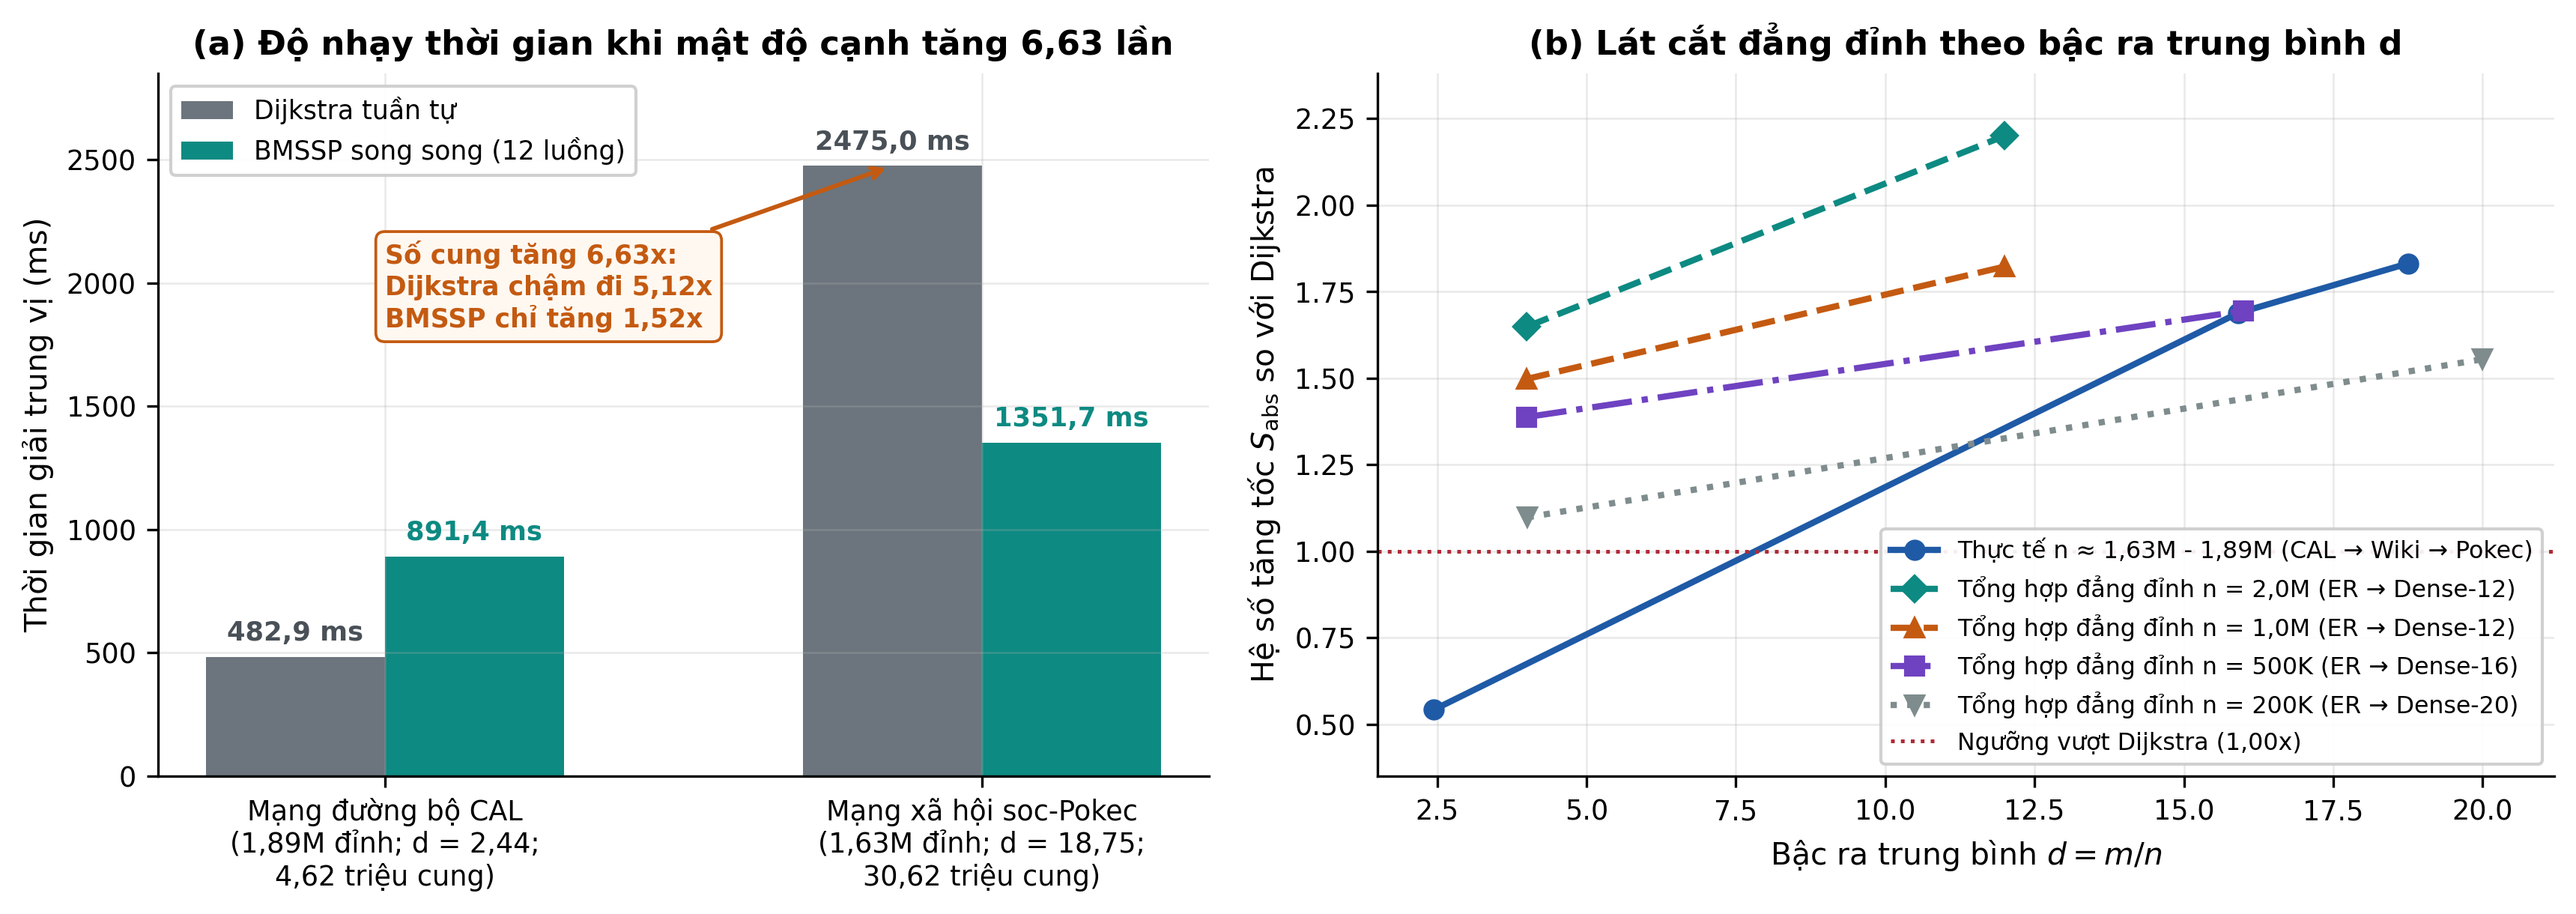
\includegraphics[width=0.96\linewidth]{image/ch3_degree_impact.png}
\caption{Độ nhạy thời gian đối lập khi mật độ cạnh tăng 6,63 lần từ mạng đường bộ \texttt{CAL} sang mạng xã hội \texttt{soc-Pokec} và các lát cắt đẳng đỉnh theo bậc trung bình $d$.}
\label{fig:degree_impact}
\end{figure}

Bằng chứng thực nghiệm rõ nét nhất thể hiện trên Hình~\ref{fig:degree_impact}a khi đối chiếu hai mạng thực tế có quy mô đỉnh tương đương khoảng $1{,}63\mathrm{M}$--$1{,}89\mathrm{M}$ là \texttt{CAL} và \texttt{soc-Pokec}: khi số cung tăng gấp $6{,}63$ lần từ $4{,}62$ triệu lên $30{,}62$ triệu cung, Dijkstra tuần tự bị chậm đi tới $5{,}12$ lần từ $482{,}93\,\mathrm{ms}$ lên $2\,474{,}98\,\mathrm{ms}$, trái lại hệ thống BMSSP ở $12$ luồng chỉ tăng thời gian đúng $1{,}52$ lần từ $891{,}43\,\mathrm{ms}$ lên $1\,351{,}73\,\mathrm{ms}$. Trên Hình~\ref{fig:degree_impact}b, mọi lát cắt giữ cố định quy mô đỉnh từ $200\mathrm{K}$ đến $2{,}0\mathrm{M}$ đều khẳng định quy luật nhất quán rằng bậc trung bình $d$ càng cao thì hệ số tăng tốc $S_{\mathrm{abs}}$ càng lớn.

\begin{figure}[!htb]
\centering
\resizebox{0.96\textwidth}{!}{%
\begin{tikzpicture}[>=latex, font=\scriptsize]
    % Biểu đồ thanh chồng ngang 100% (chiều dài thanh = 10.0 cm tương ứng 100%)
    \fill[orange!72!black] (0.0, 4.35) rectangle (0.45, 4.60);
    \node[anchor=west] at (0.55, 4.47) {Điều phối tuần tự $T_{\mathrm{seq}}(n)$};
    \fill[blue!55!black] (4.05, 4.35) rectangle (4.50, 4.60);
    \node[anchor=west] at (4.60, 4.47) {Quản lý và rút biên $\mathcal{D}$};
    \fill[teal!75!black] (7.65, 4.35) rectangle (8.10, 4.60);
    \node[anchor=west] at (8.20, 4.47) {Duyệt và thư giãn cạnh CSR song song};

    \foreach \v/\lbl in {0/0\%, 2.5/25\%, 5.0/50\%, 7.5/75\%, 10.0/100\%} {
        \draw[gray!25, thin] (\v, 0.30) -- (\v, 4.05);
        \draw[black!70] (\v, 0.30) -- (\v, 0.20);
        \node[anchor=north] at (\v, 0.16) {\lbl};
    }
    \draw[thick, black!80] (0, 0.30) -- (10.0, 0.30);

    % Hàng 1: Đồ thị nhỏ trong L3 (cit-HepPh) -> 48% + 34% + 18%
    \node[anchor=east, align=right, text width=3.4cm] at (-0.18, 3.62) {\textbf{Đồ thị nhỏ trong L3}\\(\texttt{cit-HepPh}; $34{,}5\mathrm{K}$)};
    \fill[orange!72!black] (0.00, 3.40) rectangle (4.80, 3.84); \node[text=white, font=\scriptsize\bfseries] at (2.40, 3.62) {48\%};
    \fill[blue!55!black]   (4.80, 3.40) rectangle (8.20, 3.84); \node[text=white, font=\scriptsize\bfseries] at (6.50, 3.62) {34\%};
    \fill[teal!75!black]   (8.20, 3.40) rectangle (10.00, 3.84); \node[text=white, font=\scriptsize\bfseries] at (9.10, 3.62) {18\%};

    % Hàng 2: Đường bộ biên hẹp (NW / CAL) -> 39% + 33% + 28%
    \node[anchor=east, align=right, text width=3.4cm] at (-0.18, 2.68) {\textbf{Đường bộ biên hẹp}\\(\texttt{NW}, \texttt{CAL}; $d \approx 2{,}4$)};
    \fill[orange!72!black] (0.00, 2.46) rectangle (3.90, 2.90); \node[text=white, font=\scriptsize\bfseries] at (1.95, 2.68) {39\%};
    \fill[blue!55!black]   (3.90, 2.46) rectangle (7.20, 2.90); \node[text=white, font=\scriptsize\bfseries] at (5.55, 2.68) {33\%};
    \fill[teal!75!black]   (7.20, 2.46) rectangle (10.00, 2.90); \node[text=white, font=\scriptsize\bfseries] at (8.60, 2.68) {28\%};

    % Hàng 3: Mạng Web điểm cắt (web-BerkStan) -> 22% + 31% + 47%
    \node[anchor=east, align=right, text width=3.4cm] at (-0.18, 1.74) {\textbf{Mạng Web điểm cắt}\\(\texttt{web-BerkStan}; $d = 11{,}1$)};
    \fill[orange!72!black] (0.00, 1.52) rectangle (2.20, 1.96); \node[text=white, font=\scriptsize\bfseries] at (1.10, 1.74) {22\%};
    \fill[blue!55!black]   (2.20, 1.52) rectangle (5.30, 1.96); \node[text=white, font=\scriptsize\bfseries] at (3.75, 1.74) {31\%};
    \fill[teal!75!black]   (5.30, 1.52) rectangle (10.00, 1.96); \node[text=white, font=\scriptsize\bfseries] at (7.65, 1.74) {47\%};

    % Hàng 4: Đồ thị lớn bậc cao (soc-Pokec / D12_2M) -> 12% + 24% + 64%
    \node[anchor=east, align=right, text width=3.4cm] at (-0.18, 0.80) {\textbf{Mạng lớn bậc cao}\\(\texttt{Pokec}, \texttt{D12\_2M}; $d \ge 12$)};
    \fill[orange!72!black] (0.00, 0.58) rectangle (1.20, 1.02); \node[text=white, font=\scriptsize\bfseries] at (0.60, 0.80) {12\%};
    \fill[blue!55!black]   (1.20, 0.58) rectangle (3.60, 1.02); \node[text=white, font=\scriptsize\bfseries] at (2.40, 0.80) {24\%};
    \fill[teal!75!black]   (3.60, 0.58) rectangle (10.00, 1.02); \node[text=white, font=\scriptsize\bfseries] at (6.80, 0.80) {64\%};
\end{tikzpicture}%
}
\caption{Sự dịch chuyển tỷ trọng thời gian giữa ba thành phần chi phí của Công thức~\eqref{eq:emp-bmssp} ở cấu hình 8--12 luồng qua bốn chế độ cấu trúc đồ thị.}
\label{fig:tikz_arch_regime}
\end{figure}

Sự dịch chuyển tỷ trọng của ba thành phần trong Công thức~\eqref{eq:emp-bmssp} được tổng kết trực quan trên Hình~\ref{fig:tikz_arch_regime}, qua đó chỉ rõ hai nút thắt còn giới hạn hệ số mở rộng tối đa của hệ thống. Thứ nhất, trên đồ thị nhỏ hoặc mạng đường bộ biên hẹp, phần lớn đợt duyệt rơi dưới ngưỡng $\Theta_{\mathrm{cutoff}}$ nên phần việc tuần tự $T_{\mathrm{seq}}(n)$ cùng thao tác \textsc{Pull} chiếm hơn $70\%$ tổng thời gian chạy. Thứ hai, khi chuyển sang mạng lớn bậc cao như \texttt{soc-Pokec} và \texttt{D12\_2M}, pha quét cạnh CSR song song mở rộng lên chiếm phần lớn khối lượng tính toán giúp thuật toán bứt tốc mạnh mẽ; tuy vậy, khoảng một phần ba thời gian còn lại vẫn nằm ở thao tác \textsc{Pull} tuần tự dưới khóa rút riêng kết hợp giới hạn băng thông bộ nhớ chia sẻ của $6$ lõi vật lý, giữ hệ số tự tăng tốc nội tại $S_{\mathrm{self}}$ bão hòa trong dải $1{,}84\times$--$2{,}28\times$.

\subsection{Quy luật mặt phẳng pha $(n, d)$ và miền lựa chọn thuật toán}\label{subsec:c3-phase-law}

Để tổng quát hóa định lượng kết quả trên toàn bộ $23$ bộ dữ liệu, nhóm tiến hành khớp mô hình hồi quy mặt phản ứng log-tuyến tính của hệ số tăng tốc tuyệt đối $S_{\mathrm{abs}}$ theo $\log_{10} n$, $\log_{10} d$ và đặc trưng hình học phẳng của mạng đường bộ. Như trình bày trên Hình~\ref{fig:phase_nd}b, mô hình thực nghiệm đạt hệ số xác định $R^2 = 0{,}9018$, giải thích hơn $90\%$ phương sai tốc độ quan sát được trên phần cứng thực tế.

\begin{figure}[!htb]
\centering
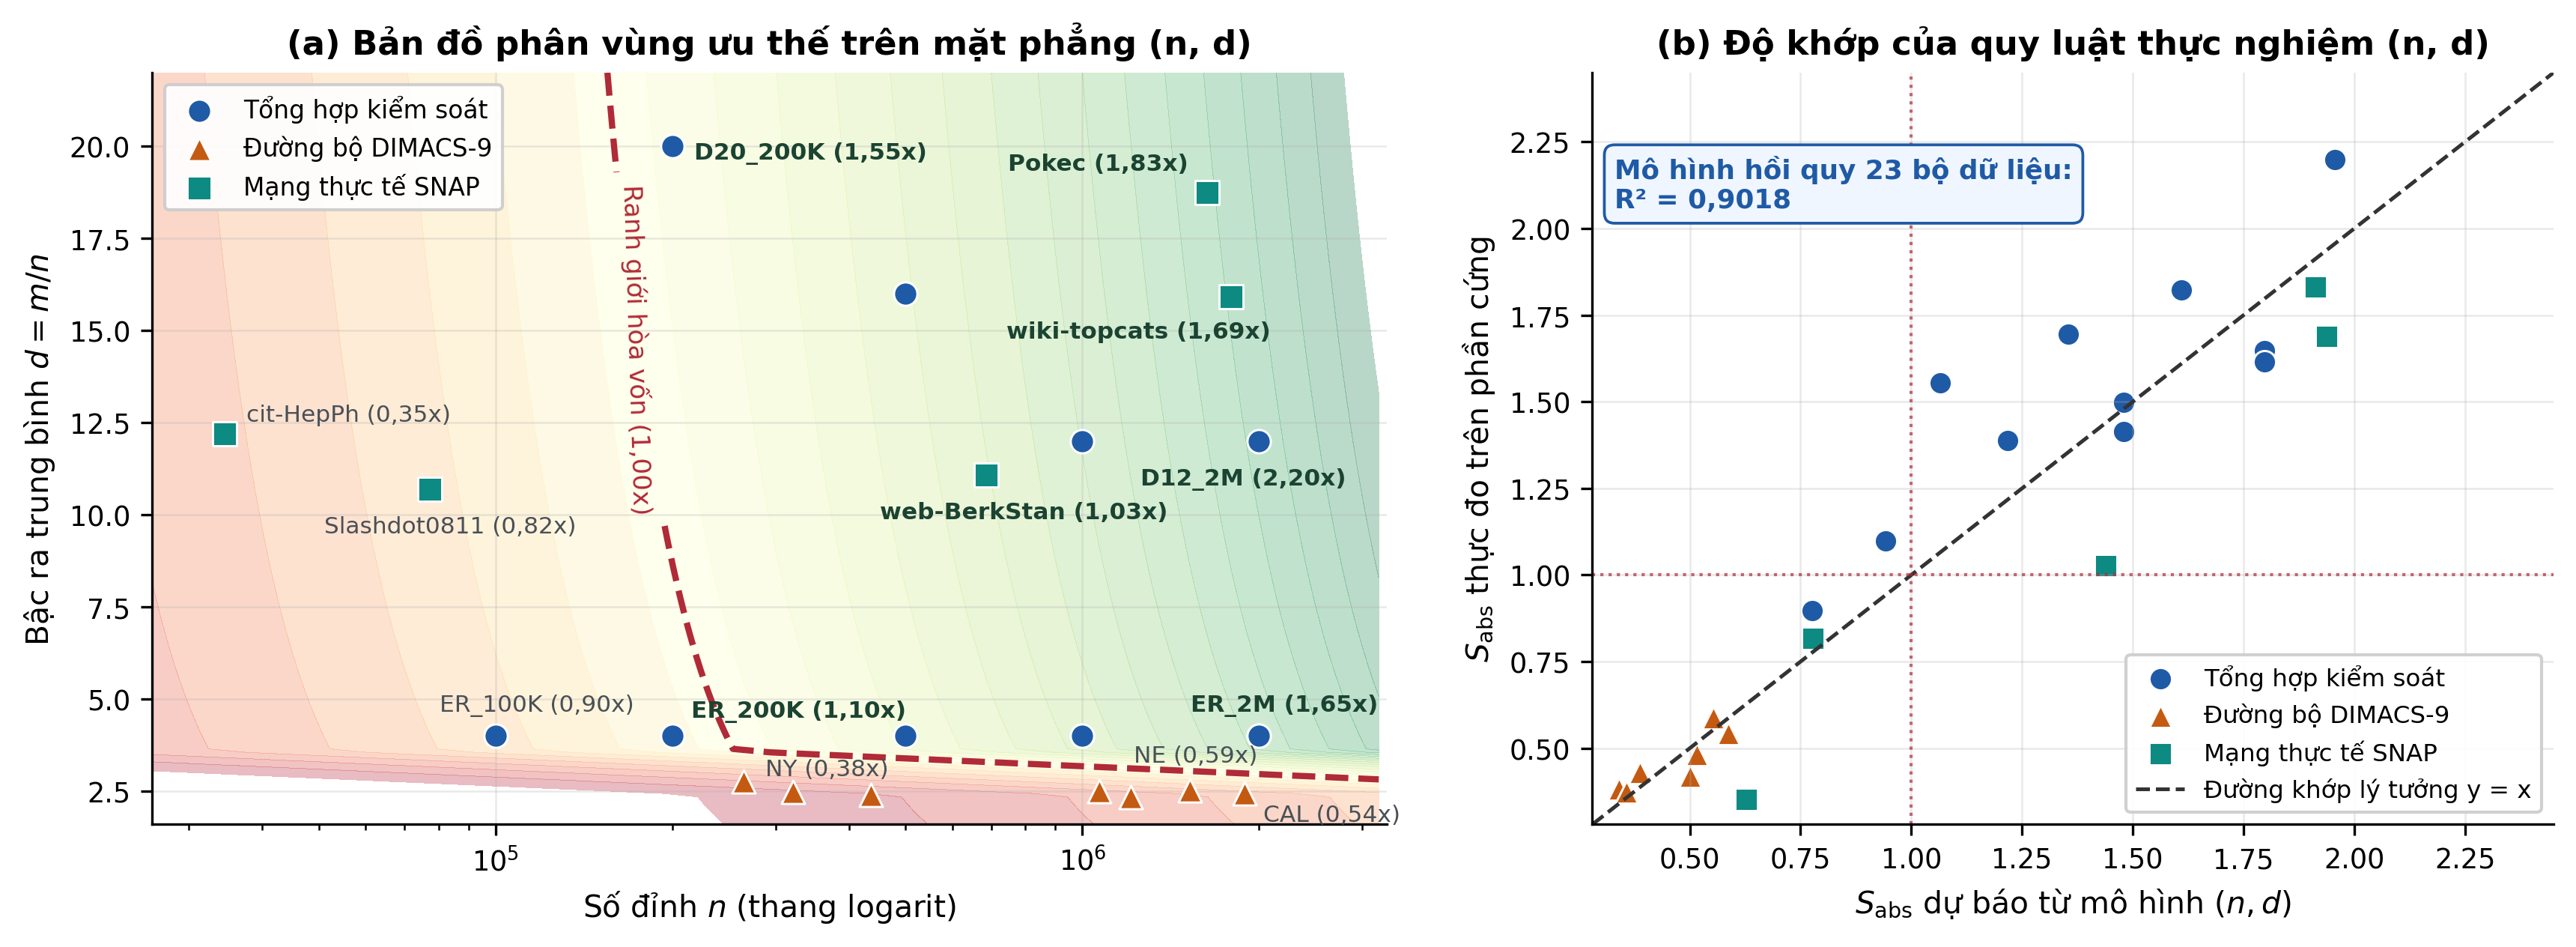
\includegraphics[width=0.96\linewidth]{image/ch3_phase_diagram_nd.png}
\caption{Bản đồ phân vùng ưu thế giữa Dijkstra tuần tự và BMSSP song song trên mặt phẳng $(n, d)$ cùng kiểm định độ khớp mô hình hồi quy trên 23 bộ dữ liệu thực nghiệm.}
\label{fig:phase_nd}
\end{figure}

Bản đồ pha trên Hình~\ref{fig:phase_nd}a phân tách không gian tham số $(n, d)$ qua đường ranh giới hòa vốn $S_{\mathrm{abs}} = 1{,}00\times$ thành hai miền ưu thế rõ rệt, được đúc kết thành quy tắc lựa chọn thực tiễn trong Bảng~\ref{tab:selection_guide}. Bên trái và phía dưới đường ranh giới là miền ưu thế của Dijkstra tuần tự, bao gồm mọi đồ thị quy mô nhỏ dưới $150\,000$ đỉnh nằm trọn trong bộ nhớ đệm và các mạng phẳng bậc cực thấp $d \le 3$ có mặt sóng mở rộng hẹp. Phía trên và bên phải đường ranh giới là miền ưu thế của BMSSP song song: trên đồ thị kết nối phân tán đều có $d \ge 4$, thuật toán vượt qua Dijkstra từ mốc $150\,000$--$200\,000$ đỉnh; trên các mạng thực tế có tính phân cụm cục bộ như Web và mạng xã hội với $d \ge 11$, điểm cắt nằm quanh mốc $450\,000$--$500\,000$ đỉnh tới được như trường hợp \texttt{web-BerkStan} và mở rộng ưu thế lên $1{,}69\times$--$2{,}20\times$ ở quy mô hàng triệu đỉnh.

\begin{table}[!htb]
\centering
{\small\setlength{\tabcolsep}{5pt}\setlength{\baselineskip}{13.5pt}
\begin{tabularx}{\textwidth}{@{} >{\raggedright\arraybackslash}p{3.65cm} >{\raggedright\arraybackslash}p{2.75cm} >{\raggedright\arraybackslash}X @{}}
\toprule
\textbf{Miền tham số $(n, d)$} & \textbf{Phương pháp ưu thế} & \textbf{Cơ sở kỹ thuật thực nghiệm} \\
\midrule
Đồ thị nhỏ $n < 150\,000$ ở mọi mức bậc $d$ & Dijkstra tuần tự & Dữ liệu nằm gọn trong bộ nhớ đệm L2 và L3, thời gian giải dưới $55\,\mathrm{ms}$ nên tránh được chi phí khởi tạo đệ quy và đồng bộ luồng. \\
\addlinespace[5pt]
Mạng phẳng hai chiều bậc rất thấp $d \le 3$ với $n \le 2\mathrm{M}$ & Dijkstra tuần tự & Mặt sóng địa lý hẹp thường xuyên rơi dưới ngưỡng $\Theta_{\mathrm{cutoff}} = 2048$, trong khi Dijkstra hưởng lợi mạnh từ tính cục bộ không gian. \\
\addlinespace[5pt]
Đồ thị trung bình $n \in [200\mathrm{K}, 700\mathrm{K}]$ có $d \ge 4$ ngẫu nhiên hoặc $d \ge 11$ thực tế & BMSSP song song $8$ luồng & Khối lượng cạnh mỗi lát đủ lớn để bù đắp chi phí điều phối, bắt đầu vượt Dijkstra với $S_{\mathrm{abs}}$ từ $1{,}03\times$ đến $1{,}69\times$. \\
\addlinespace[5pt]
Đồ thị quy mô lớn $n \ge 1\,000\,000$ có $d \ge 4$, đặc biệt mạng bậc cao $d \in [12, 20]$ & BMSSP song song $8\text{--}12$ luồng & Hàng đợi của Dijkstra tràn bộ nhớ đệm L3, còn BMSSP khai thác tốt quét CSR đa luồng, đạt $S_{\mathrm{abs}}$ từ $1{,}41\times$ đến $2{,}20\times$. \\
\bottomrule
\end{tabularx}
}
\caption{Tổng hợp miền lựa chọn thuật toán thực tiễn theo số đỉnh $n$, bậc trung bình $d$ và cấu trúc hình học đồ thị.}
\label{tab:selection_guide}
\end{table}

Cuối cùng, cần phân định trung thực về mặt học thuật rằng ưu thế tốc độ $1{,}41\times$--$2{,}20\times$ đạt được trên phần cứng thực tế là thành quả tổng hợp của việc song song hóa dữ liệu đa lõi trên kiến trúc lát khoảng cách kết hợp giảm thiểu tranh chấp trên \texttt{Concurrent\allowbreak FrontierD}, thay vì chỉ riêng cận tiệm cận tuần tự lý thuyết. Tại chế độ đơn luồng $p = 1$, cài đặt Dijkstra nhị phân vẫn nhanh hơn nhẹ từ $3\%$ đến $26\%$ trên các đồ thị lớn bậc cao nhờ cấu trúc mảng phẳng đơn giản; chính khả năng giải phóng song song hàng triệu phép thư giãn cạnh trong mỗi miền khoảng cách là yếu tố giúp BMSSP vượt lên rõ rệt trên các vi xử lý đa lõi hiện đại.

% ============================================================
% KẾT LUẬN
% ============================================================
\chapter*{KẾT LUẬN}
\addcontentsline{toc}{chapter}{Kết luận}

Tiểu luận đã nghiên cứu cơ sở lý thuyết, thiết kế kiến trúc hệ thống và triển khai hoàn chỉnh phiên bản song song của thuật toán \textit{Bounded Multi-Source Shortest Path} bằng ngôn ngữ C++20 kết hợp OpenMP cho bài toán đường đi ngắn nhất nguồn đơn trên đồ thị có hướng trọng số không âm. Bám sát mô hình đệ quy cắt lát khoảng cách của bài báo gốc, nhóm đã xây dựng kiến trúc phân bốn tầng tách biệt giao diện biên \texttt{IFrontierD} với tầng đồng bộ phần cứng, kết hợp bản ghi trạng thái đỉnh nguyên tử 128-bit tích hợp đường đọc nhanh 64-bit, cấu trúc biên hai phân vùng \texttt{Concurrent\allowbreak FrontierD} sử dụng danh sách nhảy khối kiểu B-Link có thu hồi bộ nhớ theo kỷ nguyên EBR, bể cấp phát khối cục bộ theo luồng và kỹ thuật chia tải cạnh dựa trên mảng tổng tiền tố bậc ra.

Tính đúng đắn của hệ thống được xác nhận độc lập trước khi đánh giá hiệu năng thông qua bốn bộ kiểm thử tự động chuyên sâu, bao gồm hơn $1{,}56$ triệu phép kiểm tra bất biến, bài đo chịu tải đồng thời $32$ luồng với mười triệu thao tác biên và $240$ lượt kiểm thử các trường hợp biên như chu trình trọng số $0$, đường đi gần hòa hay đỉnh siêu bậc. Trên toàn bộ $23$ bộ dữ liệu thực nghiệm trải rộng tới $2\,000\,000$ đỉnh và $30\,622\,564$ cung ở mọi cấu hình từ $1$ đến $12$ luồng, khoảng cách ngắn nhất tìm được đều trùng khớp tuyệt đối với bộ giải đối chứng Dijkstra tuần tự.

Về phương diện hiệu năng thực thi trên vi xử lý $6$ lõi $12$ luồng, nghiên cứu đã xác lập được mối liên hệ định lượng chặt chẽ với hệ số xác định $R^2 = 0{,}9018$ giữa quy mô đỉnh $n$, bậc trung bình $d = m/n$ và tốc độ tương đối của hai thuật toán. Thực nghiệm chỉ rõ trên đồ thị nhỏ dưới $150\,000$ đỉnh hoặc trên $7$ mạng giao thông đường bộ phẳng DIMACS-9 có bậc rất thấp $d \in [2{,}34;\, 2{,}76]$, mặt sóng mở rộng hẹp thường xuyên rơi dưới ngưỡng độ hạt $\Theta_{\mathrm{cutoff}} = 2048$ nên Dijkstra tuần tự vẫn giữ ưu thế tốc độ, dù tỷ số chênh lệch thu hẹp dần từ $2{,}67\times$ xuống $1{,}70\times$ khi quy mô vượt bộ nhớ đệm L3. Ngược lại, khi bậc đỉnh và quy mô tăng lên, hệ thống BMSSP song song chính thức vượt qua Dijkstra tại mốc \texttt{ER\_200K} trên dữ liệu tổng hợp và tại mạng liên kết Web \texttt{web-BerkStan} với $S_{\mathrm{abs}} = 1{,}03\times$ trên dữ liệu thực tế. Ở quy mô hàng triệu đỉnh và bậc trung bình từ $12$ đến $20$, hệ thống đạt hệ số tự tăng tốc nội tại $1{,}84\times$--$2{,}28\times$, giải nhanh hơn Dijkstra tuần tự từ $1{,}69\times$ trên \texttt{wiki-topcats}, $1{,}83\times$ trên mạng xã hội \texttt{soc-Pokec} cho đến $2{,}20\times$ trên đồ thị tổng hợp hai triệu đỉnh.

Bên cạnh những kết quả đạt được, hệ thống hiện tại vẫn tồn tại một số giới hạn kỹ thuật mở ra hướng phát triển tiếp theo. Trước hết, thao tác rút biên \textsc{Pull} và chèn tiền tố \textsc{BatchPrepend} vẫn thực thi tuần tự trên luồng điều phối nên tạo thành cận trên của đường găng khi số lõi vật lý tăng cao; việc nghiên cứu kỹ thuật rút biên và phân hoạch khối song song sẽ giúp nâng cao hơn nữa khả năng mở rộng đa luồng. Ngoài ra, các phép đo hiện mới thực hiện trên một vi xử lý máy trạm $6$ lõi vật lý với chế độ tắt biến đổi bậc hằng số mặc định; khảo sát hệ thống trên các máy chủ nhiều lõi vật lý có băng thông bộ nhớ lớn hơn, tự động thích ứng ngưỡng độ hạt $\Theta_{\mathrm{cutoff}}$ theo độ rộng mặt sóng thực tế hoặc kết hợp tăng tốc pha thư giãn cạnh mật độ cao trên GPU sẽ là những hướng mở rộng giàu tiềm năng trong tương lai.

% ============================================================
% TÀI LIỆU THAM KHẢO
% ============================================================
\newpage
\addcontentsline{toc}{chapter}{Tài liệu tham khảo}
\begin{thebibliography}{99}

\bibitem{duan2025breaking}
R. Duan, J. Mao, X. Mao, X. Shu, and L. Yin.
\textit{Breaking the Sorting Barrier for Directed Single-Source Shortest Paths.}
In Proceedings of the 57th Annual ACM Symposium on Theory of Computing (STOC '25), ACM, 2025.

\bibitem{dijkstra1959note}
E. W. Dijkstra.
\textit{A Note on Two Problems in Connexion with Graphs.}
Numerische Mathematik, 1(1):269--271, 1959.

\bibitem{bellman1958routing}
R. Bellman.
\textit{On a Routing Problem.}
Quarterly of Applied Mathematics, 16(1):87--90, 1958.

\bibitem{cormen2022introduction}
T. H. Cormen, C. E. Leiserson, R. L. Rivest, and C. Stein.
\textit{Introduction to Algorithms}, 4th edition.
The MIT Press, Cambridge, MA, 2022.

\bibitem{fredman1987fibonacci}
M. L. Fredman and R. E. Tarjan.
\textit{Fibonacci Heaps and Their Uses in Improved Network Optimization Algorithms.}
Journal of the ACM, 34(3):596--615, 1987.

\bibitem{haeupler2024universal}
B. Haeupler, R. Hlad{\'\i}k, V. Rozho{\v{n}}, R. E. Tarjan, and J. T{\v{e}}tek.
\textit{Universal Optimality of Dijkstra via Beyond-Worst-Case Heaps.}
In Proceedings of the 65th Annual IEEE Symposium on Foundations of Computer Science (FOCS), 2024.

\bibitem{frederickson1983data}
G. N. Frederickson.
\textit{Data Structures for On-Line Updating of Minimum Spanning Trees.}
In Proceedings of the 15th Annual ACM Symposium on Theory of Computing (STOC), pp. 252--257, 1983.

\bibitem{meyer2003deltastepping}
U. Meyer and P. Sanders.
\textit{$\Delta$-stepping: A Parallelizable Shortest Path Algorithm.}
Journal of Algorithms, 49(1):114--152, 2003.

\bibitem{brent1974parallel}
R. P. Brent.
\textit{The Parallel Evaluation of General Arithmetic Expressions.}
Journal of the ACM, 21(2):201--206, 1974.

\bibitem{amdahl1967validity}
G. M. Amdahl.
\textit{Validity of the Single Processor Approach to Achieving Large Scale Computing Capabilities.}
In Proceedings of the AFIPS Spring Joint Computer Conference, pp. 483--485, 1967.

\bibitem{dagum1998openmp}
L. Dagum and R. Menon.
\textit{OpenMP: An Industry-Standard API for Shared-Memory Programming.}
IEEE Computational Science and Engineering, 5(1):46--55, 1998.

\bibitem{openmp52}
OpenMP Architecture Review Board.
\textit{OpenMP Application Programming Interface, Version 5.2.}
November 2021. \url{https://www.openmp.org/specifications/}

\bibitem{saad2003iterative}
Y. Saad.
\textit{Iterative Methods for Sparse Linear Systems}, 2nd edition.
Society for Industrial and Applied Mathematics (SIAM), 2003.

\bibitem{shun2013ligra}
J. Shun and G. E. Blelloch.
\textit{Ligra: A Lightweight Graph Processing Framework for Shared Memory.}
In Proceedings of the 18th ACM SIGPLAN Symposium on Principles and Practice of Parallel Programming (PPoPP '13), pp. 135--146, 2013.

\bibitem{herlihy2012art}
M. Herlihy and N. Shavit.
\textit{The Art of Multiprocessor Programming}, Revised 1st edition.
Morgan Kaufmann, 2012.

\bibitem{intel2023sdm}
Intel Corporation.
\textit{Intel\textsuperscript{\textregistered} 64 and IA-32 Architectures Software Developer's Manual, Volume 2: Instruction Set Reference.}
2023.

\bibitem{berger2000hoard}
E. D. Berger, K. S. McKinley, R. D. Blumofe, and P. R. Wilson.
\textit{Hoard: A Scalable Memory Allocator for Multithreaded Applications.}
In Proceedings of the 9th International Conference on Architectural Support for Programming Languages and Operating Systems (ASPLOS IX), pp. 117--128, 2000.

\bibitem{blelloch1990prefix}
G. E. Blelloch.
\textit{Prefix Sums and Their Applications.}
Technical Report CMU-CS-90-190, School of Computer Science, Carnegie Mellon University, 1990.

\bibitem{tsigas2003parallel}
P. Tsigas and Y. Zhang.
\textit{A Simple, Fast Parallel Implementation of Quicksort and its Performance Evaluation on SUN Enterprise 10000.}
In Proceedings of the 11th Euromicro Conference on Parallel, Distributed and Network-Based Processing (PDP '03), pp. 372--381, 2003.

\bibitem{serebryany2009threadsanitizer}
K. Serebryany and T. Iskhodzhanov.
\textit{ThreadSanitizer -- Data Race Detection in Practice.}
In Proceedings of the Workshop on Binary Instrumentation and Applications (WBIA '09), pp. 62--71, 2009.

\bibitem{pugh1990skip}
W. Pugh.
\textit{Skip Lists: A Probabilistic Alternative to Balanced Trees.}
Communications of the ACM, 33(6):668--676, 1990.

\bibitem{lehman1981efficient}
P. L. Lehman and S. B. Yao.
\textit{Efficient Locking for Concurrent Operations on B-Trees.}
ACM Transactions on Database Systems (TODS), 6(4):650--670, 1981.

\bibitem{demetrescu2009dimacs}
C. Demetrescu, A. V. Goldberg, and D. S. Johnson.
\textit{The Shortest Path Problem: Ninth DIMACS Implementation Challenge.}
DIMACS Book Series, Vol. 74, American Mathematical Society, 2009.

\bibitem{leskovec2014snap}
J. Leskovec and A. Krevl.
\textit{SNAP Datasets: Stanford Large Network Dataset Collection.}
June 2014. \url{http://snap.stanford.edu/data}

\end{thebibliography}
\end{document}
